\documentclass[11pt]{article}
\usepackage{a4wide}
%\raggedright
%\usepackage{driverbook}
\usepackage{latexsym}           % math symbols that were omitted in latex2e
\usepackage{amsbsy}             % bold greek defs
\usepackage{amsmath,graphicx}
\usepackage{bbm}
\usepackage{mathrsfs}
\usepackage{stmaryrd}
\usepackage{graphics}
\usepackage{acronym}
\usepackage{longtable}
\usepackage{mathtools}
\usepackage{times}
\usepackage{setspace}
\usepackage{cite}
\usepackage{array}
\usepackage{subfigure}
\usepackage{amsmath,amsthm}
\usepackage{amssymb}
\usepackage{wasysym,url}
\usepackage{fixltx2e,amsmath}
\usepackage{setspace,float}
\usepackage{color}
\usepackage{cases,bm}
\usepackage{mathrsfs}
\usepackage{enumitem}
\usepackage{hyperref}
\usepackage{mathtools,cuted}
\usepackage[linesnumbered,ruled,vlined]{algorithm2e}
\usepackage{epsfig}
\usepackage{color}
\DontPrintSemicolon

\usepackage{geometry}
 \geometry{
 a4paper,
 total={170mm,257mm},
 left=20mm,
 top=30mm,
 bottom=30mm,
 }
 
 
\usepackage{listings}
\usepackage{xcolor}

\definecolor{codegreen}{rgb}{0,0.6,0}
\definecolor{codegray}{rgb}{0.5,0.5,0.5}
\definecolor{codepurple}{rgb}{0.58,0,0.82}
\definecolor{backcolour}{rgb}{0.95,0.95,0.92}

\lstdefinestyle{mystyle}{
    backgroundcolor=\color{backcolour},   
    commentstyle=\color{codegreen},
    keywordstyle=\color{magenta},
    numberstyle=\tiny\color{codegray},
    stringstyle=\color{codepurple},
    basicstyle=\ttfamily\footnotesize,
    breakatwhitespace=false,         
    breaklines=true,                 
    captionpos=b,                    
    keepspaces=true,                 
    numbers=left,                    
    numbersep=5pt,                  
    showspaces=false,                
    showstringspaces=false,
    showtabs=false,                  
    tabsize=2
}

\lstset{style=mystyle}

\newcommand{\by}{\mathbf{y}}
\newcommand{\br}{\mathbf{r}}
\newcommand{\bv}{\mathbf{v}}
\newcommand{\bh}{\mathbf{h}}
\newcommand{\bx}{\mathbf{x}}
\newcommand{\bs}{\mathbf{s}}
\newcommand{\bw}{\mathbf{w}}
\newcommand{\bR}{\mathbf{R}}
\newcommand{\bI}{\mathbf{I}}
\newcommand{\bA}{\mathbf{A}}
\newcommand{\bK}{\mathbf{K}}
\newcommand{\bQ}{\mathbf{Q}}
\newcommand{\bP}{\mathbf{P}}
\newcommand{\bC}{\mathbf{C}}
\newcommand{\rr}{\mathbb{R}}
\newcommand{\zz}{\mathbb{Z}}
\newcommand{\nn}{\mathbb{N}}
\newcommand{\cc}{\mathbb{C}}
\newcommand{\Ex}{\mathbb{E}}
\newcommand{\TT}{\mathsf{T}}
\newcommand{\HH}{\mathsf{H}}
\newcommand{\cH}{\mathcal{H}}
\newcommand{\cN}{\mathcal{N}}
\newcommand{\dd}{\mathrm{d}}
\newcommand{\Prob}{\mathrm{Pr}}
\newcommand{\jj}{\mathrm{j}}

\newcommand{\zerovec}{\boldsymbol{0}}
\newcommand{\bSigma}{\boldsymbol{\Sigma}}
\newcommand{\btheta}{\boldsymbol{\theta}}
\newcommand{\bgamma}{\boldsymbol{\gamma}}

\begin{document}
\thispagestyle{empty}

{\small
\begin{flushleft}
   Name: Abijith J. Kamath\\
   Student Id: 17788
\end{flushleft}
}
\vspace{2ex}
\begin{center}
    {\Large\bf E1 244: Detection and Estimation}\\
    February-May 2021

\vspace{5mm}
{\bf Solution -- Final Project}
\end{center}
\vspace{5mm}

% -----------------------------------------------------------------------------------------------------------------------
% -----------------------------------------------------------------------------------------------------------------------

\section*{Introduction}

Automating a driving test can be done using a vehicle tracking algorithm from some measurements of the vehicle and analysing the path. A naive approach is to use the path to ensure the driver has maintained the path and avoided crashes. This does not ensure aspects like following lane rules, traffic signs, maintaining optimal speed, and other important driving ethics are being followed, but it is sufficient to make sure the driver is able to follow a given path.

\begin{figure}[h!]
	\centering
	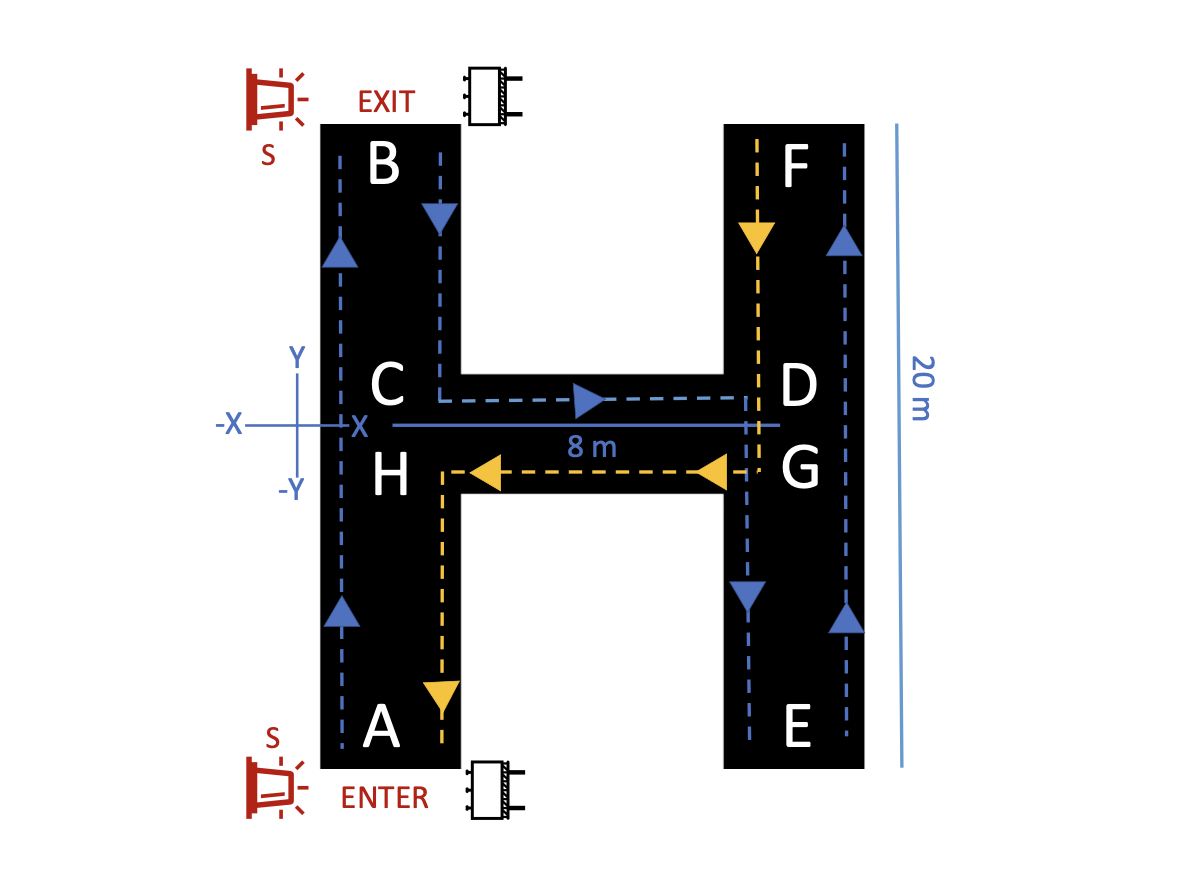
\includegraphics[width=3.5in]{../results/path.png}
\caption{Track defined for the driving test.}
\label{fig:path}
\end{figure}
Consider the track shown in Figure \ref{fig:path}. The path to be taken by the vehicle is defined to be A-B-C-D-E-F-G-H-A. The vehicle position and velocities are measured using a RADAR, that helps to continuously track the vehicle in real time. The RADAR switched ON only when the detector at the entry point A detects a vehicle, and it remains ON until the detector at the exit point B detects a vehicle. The detectors are designed using light-dependent diodes (LDR) that are: excited by a source when there is no vehicle blocking the source, which can help in differentiating between states of vehicle being present and not present. The detection problem is to design appropriate detectors at the entry and the exit, and the estimation problem is to track the vehicle using the noisy RADAR measurements.

% -----------------------------------------------------------------------------------------------------------------------
% -----------------------------------------------------------------------------------------------------------------------

\section{Part A: Vehicle Detection}
\label{sec:partA_Detection}

\subsection{Derivation}
\label{subsec:partA_derivation}

The detectors are built using LDRs, where a sensor measures voltages across the LDR. Voltage measurements $x_{m}[n], \; n=0,1,\cdots,N-1$ are made at $M$ such sensors with labels $m=1,2,\cdots,M$. Hence, the output of the sensors are:
\begin{equation}
	x_{m}[n] = \begin{cases}
		A + B_{t} + w_{m}[n], &\text{vehicle absent}, \\
		B_{t} + w_{m}[n], & \text{vehicle present},
	\end{cases}
\label{eq:LDRout}
\end{equation}
where $A$ is the voltage due to the source, $B_{t}$ is the voltage due to ambient light at some time $t$, and $w_{m}[n]$ are i.i.d zero mean, white Gaussian noise with variance $\sigma^{2}$, at the $m$th sensor. Therefore, detection of the vehicle is a hypothesis testing problem between two hypothesis:
\begin{equation}
\begin{split}
	\text{(vehicle absent) } &\cH_{0}: x_{m}[n] = A + B_{t} + w_{m}[n], \\
	\text{(vehicle present) } &\cH_{1}: x_{m}[n] = B_{t} + w_{m}[n], n=0,1,\cdots,N-1; m=1,2,\cdots,M.
\end{split}
\label{eq:hypothesis}
\end{equation}

Let $\bx$ be the vectorised measurements of dimension $NM$ (for simplicity, the derivations further take $M=1$). The joint distribution of the measurements $p_{X}(\bx)$ is a Gaussian distribution with variance $\sigma^{2}$ and mean $A+B_{t}$ under $\cH_{0}$, and $B_{t}$ under $\cH_{1}$. We will assume that we know some knowledge of $B_{t}$ for some times during the day.

% -----------------------------------------------------------------------------------------------------------------------

\subsubsection{Detector at the entry for a given $B_{t}$}
\label{subsubsec:entryDetector}

The detector at the entry is designed such that the probability of false alarm is the least, given the probability of detection is set to a constant. Such detectors maybe termed constant detection rate (CDR) detectors. Let the detector divide $\rr$ into regions of decision $R_{0}$ and $R_{1}$ corresponding hypothesis $\cH_{0}$ and $\cH_{1}$, respectively. The regions are mutually exclusive and exhaustive, i.e., $R_{0} \cup R_{1} = \rr$ and $R_{0} \cap R_{1} = \emptyset$. The CDR detector with probability of detection $P_{D} = \int_{R_{1}} p_{X}(\bx;\cH_{1}) \dd\bx$ and $P_{FA} = \int_{R_{1}} p_{X}(\bx;\cH_{0}) \dd\bx$ solves:
\begin{equation}
\begin{split}
	\underset{R_{1}}{\text{minimise }}& P_{FA}, \\
	\text{subject to }& P_{D} = \beta.
\end{split}
\label{eq:CDRopt}
\end{equation}

Consider the Lagrangian with multiplier $\lambda$:
\begin{equation}
\begin{split}
	\mathcal{L} &= P_{FA} + \lambda (P_{D}-\beta) \\
	&= \int_{R_{1}} \left( p_{X}(\bx;\cH_{0}) + \lambda p_{X}(\bx;\cH_{1}) \right) \dd\bx - \lambda\beta.
\end{split}
\label{eq:CDRLag}
\end{equation}
The minimiser of $\mathcal{L}$ also minimises $P_{FA}$ and includes points $\bx$ in $R_{1}$ such that $p_{X}(\bx;\cH_{0}) + \lambda p_{X}(\bx;\cH_{1}) < 0$. This gives the ratio test for detection: decide on $\cH_{1}$ if:
\begin{equation}
	L_{ent}(\bx) = \frac{p_{X}(\bx;\cH_{0})}{p_{X}(\bx;\cH_{1})} < -\lambda = \gamma,
\label{eq:CDRratioTest}
\end{equation}
which is a ratio test that compares the ratio of likelihoods of the two hypothesis to some threshold $\gamma$ that is decided using the condition $P_{D}=\beta$. Such a ratio test gives simple regions $R_{0}$ and $R_{1}$ that is parametrised by a threshold $\gamma$. This is similar to the Neymann-Pearson detector, where $P_{FA}$ is held constant and $P_{D}$ is maximised, and a similar ratio test is obtained.

Consider the test under the hypothesis in (\ref{eq:hypothesis}). The likelihood ratio admits:
\begin{equation}
\begin{split}
	L_{ent}(\bx) &= \frac{p_{X}(\bx; \cH_{0})}{p_{X}(\bx; \cH_{1})}, \\
&= \frac{\frac{1}{(2\pi\sigma^{2})^{N/2}} \mathrm{exp}\left(-\frac{1}{2\sigma^{2}} \sum_{n=0}^{N-1} (x_{m}[n] - A - B_{t})^{2} \right)}{\frac{1}{(2\pi\sigma^{2})^{N/2}} \mathrm{exp}\left(-\frac{1}{2\sigma^{2}} \sum_{n=0}^{N-1} (x_{m}[n] - B_{t})^{2} \right)}, \\
\implies \ln L_{ent}(\bx) &= -\frac{1}{2\sigma^{2}} \left( -2A \sum_{n=0}^{N-1}x_{m}[n] + NA^{2} + 2NAB_{t} \right).
\end{split}
\label{eq:CDRlnTest}
\end{equation}
Since $\ln(\cdot)$ is an increasing function, the ratio test is equivalent to $\ln L_{ent}(\bx) < \ln\gamma$, which gives the test statistic:
\begin{equation}
	T(\bx) = \frac{1}{N} \sum_{n=0}^{N-1}x_{m}[n] < \frac{2\sigma^{2}\ln\gamma + NA^{2} + 2NAB_{t}}{2NA} = \gamma'.
\label{eq:CDRtestStat}
\end{equation}
The test statistic is the sample mean of the measurements. Since the measurements are i.i.d, the test statistic also has a Gaussian distribution:
\begin{equation}
	T(\bx) \sim \begin{cases}
	\cN(A+B_{t}, \frac{\sigma^{2}}{N}), & \text{under }\cH_{0}, \\
	\cN(B_{t}, \frac{\sigma^{2}}{N}), & \text{under }\cH_{1}.
	\end{cases}
\label{eq:CDRstatDist}
\end{equation}
The constant probability of detection condition $\displaystyle \beta = \Prob[T(\bx) < \gamma';\cH_{1}] = 1-Q\left( \frac{\gamma'-B_{t}}{\sqrt{\sigma^{2}/N}} \right)$ gives:
\begin{equation}
	\gamma' = \sqrt{\frac{\sigma^{2}}{N}} Q^{-1}(1-\beta) + B_{t},
\label{eq:CDRthreshold}
\end{equation}
where $Q(\cdot)$ is the survival function of the standard normal distribution. The theoretical probability of false alarm $\displaystyle P_{FA} = \Prob[T(\bx) < \gamma';\cH_{0}] = 1-Q\left( \frac{\gamma'-A-B_{t}}{\sqrt{\sigma^{2}/N}} \right)$.

% -----------------------------------------------------------------------------------------------------------------------

\subsubsection{Detector at the entry with unknown $B_{t}$}
\label{subsubsec:entryDetectorGeneralised}

The CDR detector is completely described by its threshold, and the threshold derived in (\ref{eq:CDRthreshold}) that minimises the probability of false alarm, depends on the knowledge of $B_{t}$. If $B_{t}$ is not exactly known, the probability of detection may not remain a constant. In such scenarios, methods of composite hypothesis testing like generalised likelihood ratio test are used. However, in this case, since the range of possible values that $B_{t}$ takes is known, the solution can be inferred from the threshold derived in (\ref{eq:CDRthreshold}).

Note that, for any choice of $B_{t}$, the theoretical probability of false alarm:
\begin{equation}
\begin{split}
	P_{FA} &= \Prob[T(\bx) < \gamma';\cH_{0}], \\
	&= 1-Q\left( \frac{\gamma'-A-B_{t}}{\sqrt{\sigma^{2}/N}} \right), \\
	&= 1-Q\left( Q^{-1}(1-\beta) -\sqrt{\frac{NA^{2}}{\sigma^{2}}} \right),
\end{split}
\label{eq:CDRpfa}
\end{equation}
is independent of $B_{t}$, and hence, the choice of $B_{t}$ does not change the optimal solution. Since the threshold still depends on $B_{t}$, the equality constraint $P_{D}=\beta$ cannot be maintained. Under the conditions of the problem, it is sufficient to maintain $P_{D} \geq \beta$. This can be ensured by picking the largest possible choice for the threshold, where, the probability of detection may increase, but the probability of false alarm remains the same, since it is independent of $B_{t}$. This is achieved by setting the threshold:
\begin{equation}
	\gamma' = \sqrt{\frac{\sigma^{2}}{N}} Q^{-1}(1-\beta) + B_{\text{max}},
\label{eq:generalCDRthreshold}
\end{equation}
where it is known that $B_{t}<B_{\text{max}}$ over the entire duration when testing is allowed. The detector at the entry ($D_{\text{entry}}$) is completely specified by the threshold given in (\ref{eq:generalCDRthreshold}), which constrains the probability of detection to be bounded below by $\beta$, and the probability of false alarm, as given by (\ref{eq:CDRpfa}), to be the least with that constraint.

% -----------------------------------------------------------------------------------------------------------------------

\subsubsection{Detector at the exit for a given $B_{t}$}
\label{subsubsec:exitDetector}

The detector at the exit is designed such that the probability of detection is the maximum, given the probability of false alarm is set to a constant. Such a detector is called a constant false-alarm (CFAR) detector, and the optimal detector is the Neymann-Pearson detector. Let the detector divide $\rr$ into regions of decision $R_{0}$ and $R_{1}$ corresponding hypothesis $\cH_{0}$ and $\cH_{1}$, respectively. The regions are mutually exclusive and exhaustive, i.e., $R_{0} \cup R_{1} = \rr$ and $R_{0} \cap R_{1} = \emptyset$. The CFAR detector with probability of detection $P_{D} = \int_{R_{1}} p_{X}(\bx;\cH_{1}) \dd\bx$ and $P_{FA} = \int_{R_{1}} p_{X}(\bx;\cH_{0}) \dd\bx$ solves:
\begin{equation}
\begin{split}
	\underset{R_{1}}{\text{maximise }}& P_{D}, \\
	\text{subject to }& P_{FA} = \alpha.
\end{split}
\label{eq:CFARopt}
\end{equation}

Consider the Lagrangian with multiplier $\lambda$:
\begin{equation}
\begin{split}
	\mathcal{L} &= P_{D} + \lambda (P_{FA}-\alpha) \\
	&= \int_{R_{1}} \left( p_{X}(\bx;\cH_{1}) + \lambda p_{X}(\bx;\cH_{0}) \right) \dd\bx - \lambda\alpha.
\end{split}
\label{eq:CFARLag}
\end{equation}
The maximiser of $\mathcal{L}$ also maximises $P_{D}$ and includes points $\bx$ in $R_{1}$ such that $p_{X}(\bx;\cH_{1}) + \lambda p_{X}(\bx;\cH_{0}) > 0$. This gives the ratio test for detection: decide on $\cH_{1}$ if:
\begin{equation}
	L_{ext}(\bx) = \frac{p_{X}(\bx;\cH_{1})}{p_{X}(\bx;\cH_{0})} > -\lambda = \xi,
\label{eq:CFARratioTest}
\end{equation}
which is a ratio test that compares the ratio of likelihoods of the two hypothesis to some threshold $\xi$ that is decided using the condition $P_{FA}=\alpha$. This is also a ratio rest that gives simple regions $R_{0}$ and $R_{1}$ that is parametrised by $\xi$. This is the Neymann-Pearson detector. The CDR detector in (\ref{eq:CDRratioTest}) and CFAR detector in (\ref{eq:CFARratioTest}) are similar, but the thresholds are decided using different conditions, that yield different thresholds.

Consider the test under the hypothesis in (\ref{eq:hypothesis}). The likelihood ratio admits:
\begin{equation}
\begin{split}
	L_{ext}(\bx) &= \frac{p_{X}(\bx; \cH_{1})}{p_{X}(\bx; \cH_{0})}, \\
&= \frac{\frac{1}{(2\pi\sigma^{2})^{N/2}} \mathrm{exp}\left(-\frac{1}{2\sigma^{2}} \sum_{n=0}^{N-1} (x_{m}[n] - B_{t})^{2} \right)}{\frac{1}{(2\pi\sigma^{2})^{N/2}} \mathrm{exp}\left(-\frac{1}{2\sigma^{2}} \sum_{n=0}^{N-1} (x_{m}[n] - A - B_{t})^{2} \right)}, \\
\implies \ln L_{ext}(\bx) &= -\frac{1}{2\sigma^{2}} \left( 2A \sum_{n=0}^{N-1}x_{m}[n] - NA^{2} - 2NAB_{t} \right).
\end{split}
\label{eq:CDRlnTest}
\end{equation}
Since $\ln(\cdot)$ is an increasing function, the ratio test is equivalent to $\ln L_{ext}(\bx) > \ln\xi$, which gives the same test statistic as in (\ref{eq:CDRtestStat}):
\begin{equation}
	T(\bx) = \frac{1}{N} \sum_{n=0}^{N-1}x_{m}[n] < \frac{-2\sigma^{2}\ln\xi + NA^{2} + 2NAB_{t}}{2NA} = \xi'.
\label{eq:CFARtestStat}
\end{equation}
The test statistic is the sample mean of the measurements and has the same distribution as in (\ref{eq:CDRstatDist}). The constant false-alarm condition $\displaystyle \alpha = \Prob[T(\bx) < \xi';\cH_{0}] = 1-Q\left( \frac{\xi'-A-B_{t}}{\sqrt{\sigma^{2}/N}} \right)$ gives:
\begin{equation}
	\xi' = \sqrt{\frac{\sigma^{2}}{N}} Q^{-1}(1-\alpha) + A + B_{t}.
\label{eq:CFARthreshold}
\end{equation}
The theoretical probability of detection $\displaystyle P_{D} = \Prob[T(\bx) < \gamma';\cH_{1}] = 1-Q\left( \frac{\gamma'-B_{t}}{\sqrt{\sigma^{2}/N}} \right)$.

% -----------------------------------------------------------------------------------------------------------------------

\subsubsection{Detector at the exit with unknown $B_{t}$}
\label{subsubsec:exitDetectorGeneralised}

The CFAR detector is completely described by its threshold, and the threshold derived in (\ref{eq:CFARthreshold}) that maximises the probability of detection, depends on the knowledge of $B_{t}$. If $B_{t}$ is not exactly known, similar to the case described in Section \ref{subsubsec:entryDetectorGeneralised} the probability of false alarm may not remain a constant.

Note that, for any choice of $B_{t}$, the theoretical probability of detection:
\begin{equation}
\begin{split}
	P_{D} &= \Prob[T(\bx) < \xi';\cH_{1}], \\
	&= 1-Q\left( \frac{\xi'-B_{t}}{\sqrt{\sigma^{2}/N}} \right), \\
	&= 1-Q\left( Q^{-1}(1-\alpha) -\sqrt{\frac{NA^{2}}{\sigma^{2}}} \right),
\end{split}
\label{eq:CFARpd}
\end{equation}
is independent of $B_{t}$, and hence, the choice of $B_{t}$ does not change the optimal solution. Since the threshold still depends on $B_{t}$, the equality constraint $P_{FA}=\alpha$ cannot be maintained. Under the conditions of the problem, it is sufficient to maintain $P_{FA} \leq \alpha$. This can be ensured by picking the smallest possible choice for the threshold, where, the probability of false alarm may decrease, but the probability of detection remains the same, since it is independent of $B_{t}$. This is achieved by setting the threshold:
\begin{equation}
	\xi' = \sqrt{\frac{\sigma^{2}}{N}} Q^{-1}(1-\alpha) + A + B_{\text{min}},
\label{eq:generalCFARthreshold}
\end{equation}
where it is known that $B_{t}>B_{\text{min}}$ over the entire duration when testing is allowed. The detector at the exit ($D_{\text{exit}}$) is completely specified by the threshold given in (\ref{eq:generalCFARthreshold}), which constrains the probability of false alarm to be bounded above by $\alpha$, and the probability of detection, as given by (\ref{eq:CFARpfa}), to be the highest with that constraint.

% -----------------------------------------------------------------------------------------------------------------------

\subsubsection{Locally Most Powerful detector at the exit}
\label{subsubsec:exitLMPdetector}

Section \ref{subsubsec:exitDetector} derives the Neymann-Pearson detector for hypothesis testing, where the hypothesis are as in (\ref{eq:hypothesis}). Since the noise is i.i.d Gaussian distributed, the two hypotheses can be reformulated as mean-detection problem with $\bx \sim \cN(\mu, \sigma^{2})$ and:
\begin{equation}
\begin{split}
	\text{(vehicle absent) } &\cH_{0}: \mu = B_{t}, \\
	\text{(vehicle present) } &\cH_{1}: \mu > B_{t},
\end{split}
\label{eq:LMPhypothesis}
\end{equation}
since it is known that the voltage drop due to the source $A>0$. This is a one-sided hypothesis test, and is amenable to the locally most-powerful (LMP) test. The data has a Gaussian distribution $p_{X}(\bx;\mu)$ that is parametrised by the mean, depending on the hypothesis. The LMP uses the test statistic:
\begin{equation}
	T_{\text{LMP}}(\bx) = \frac{1}{\sqrt{I(B_{t})}} \frac{\partial}{\partial \mu} \ln p_{X}(\bx;B_{t}),
\label{eq:LMPtestStat}
\end{equation}
where $I(\cdot)$ is the Fisher information of $\mu$ on $p_{X}$. The derivatives of the log-likelihood function are computed as:
\begin{equation}
\begin{split}
	\ln p_{X}(\bx;\mu) &= -\frac{N}{2}\ln(2\pi\sigma^{2}) - \frac{1}{2\sigma^{2}} \sum_{n=0}^{N-1} \left( x_{m}[n] - \mu \right)^{2}, \\
	\implies \frac{\partial}{\partial \mu} \ln p_{X}(\bx;\mu) &= \frac{1}{\sigma^{2}} \sum_{n=0}^{N-1} \left( x_{m}[n] - \mu \right), \\
	\implies \frac{\partial^{2}}{\partial \mu^{2}} \ln p_{X}(\bx;\mu) &= -\frac{N}{\sigma^{2}}.
\end{split}
\label{eq:LMPderivative}
\end{equation}
The Fisher information $I(\mu) = -\Ex[\frac{\partial^{2}}{\partial \mu^{2}} \ln p_{X}(\bx;\mu)] = \frac{N}{\sigma^{2}}$. Using this in (\ref{eq:LMPtestStat}), the test statistic $T_{\text{LMP}}(\bx) = \frac{1}{\sqrt{N\sigma^{2}}} \sum_{n=0}^{N-1}\left( x_{m}[n] - B_{t} \right)$. The LMP detector decides on the hypothesis $\cH_{1}$ if $T_{\text{LMP}}(\bx) > \eta$, where $\eta$ is some threshold chosen using the problem constraints, for example, constant false-alarm rate as in Section \ref{subsubsec:exitDetector}. The test statistic $T_{\text{LMP}}(\bx)$ depends on the data only in the sample mean, as in (\ref{eq:CFARtestStat}), i.e., the two detectors have identical test statistics. If the constraints are the same, the LMP detector is identical to the Neymann-Pearson detector.

% -----------------------------------------------------------------------------------------------------------------------
% -----------------------------------------------------------------------------------------------------------------------

\subsection{Implementation}
\label{subsec:partA_implementation}

We simulate the source with $A=1$, and consider detection during six time instants during the day where the ambient light gives $B_{t} \in \{0.1, 0.2, 0.3, 0.4, 0.5, 0.6\}$. We consider $N=5$ measurements from each sensor for both detectors and consider the effect of varying the number of sensors from $M=1,2,3$.

% -----------------------------------------------------------------------------------------------------------------------

\subsubsection{Monte-Carlo simulations for $D_{\text{entry}}$}
\label{subsubsec:entryDetector_working}

We implement $D_{\text{entry}}$ using the threshold (\ref{eq:generalCDRthreshold}), and perform Monte-Carlo simulations averaged over $10000$ realisations to estimate the probability of detection $\hat{P}_{D}$. We repeat the experiment for the six values of $B_{t}$ considered and vary $M=1,2,3$ in each case.
\begin{figure}[h!]
\centering
\subfigure[$B_{t}=0.1$]{\label{fig:a}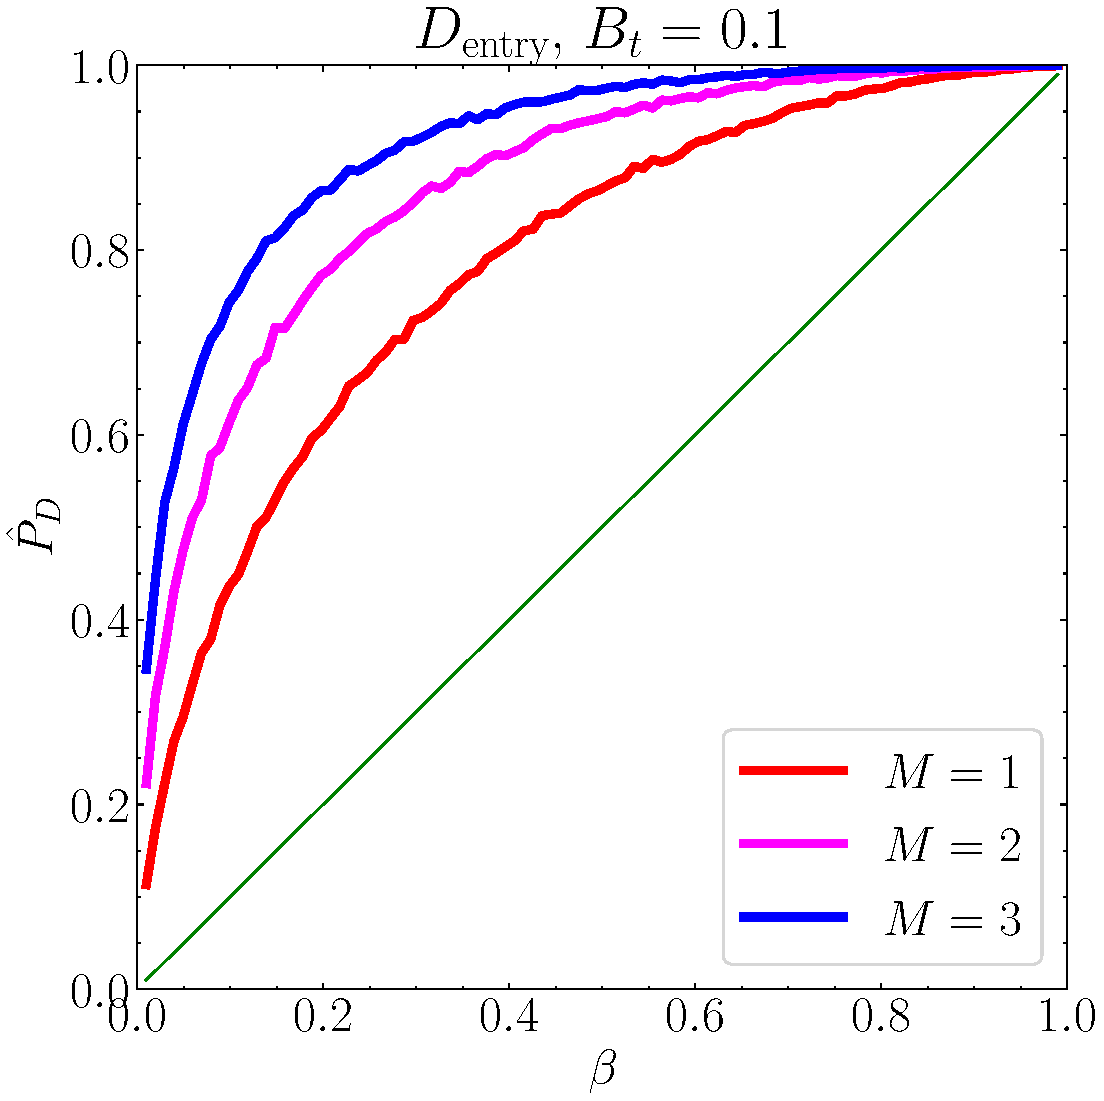
\includegraphics[width=2in]{../results/CDR/CDR_PD_Bt_0.1}}
\subfigure[$B_{t}=0.2$]{\label{fig:a}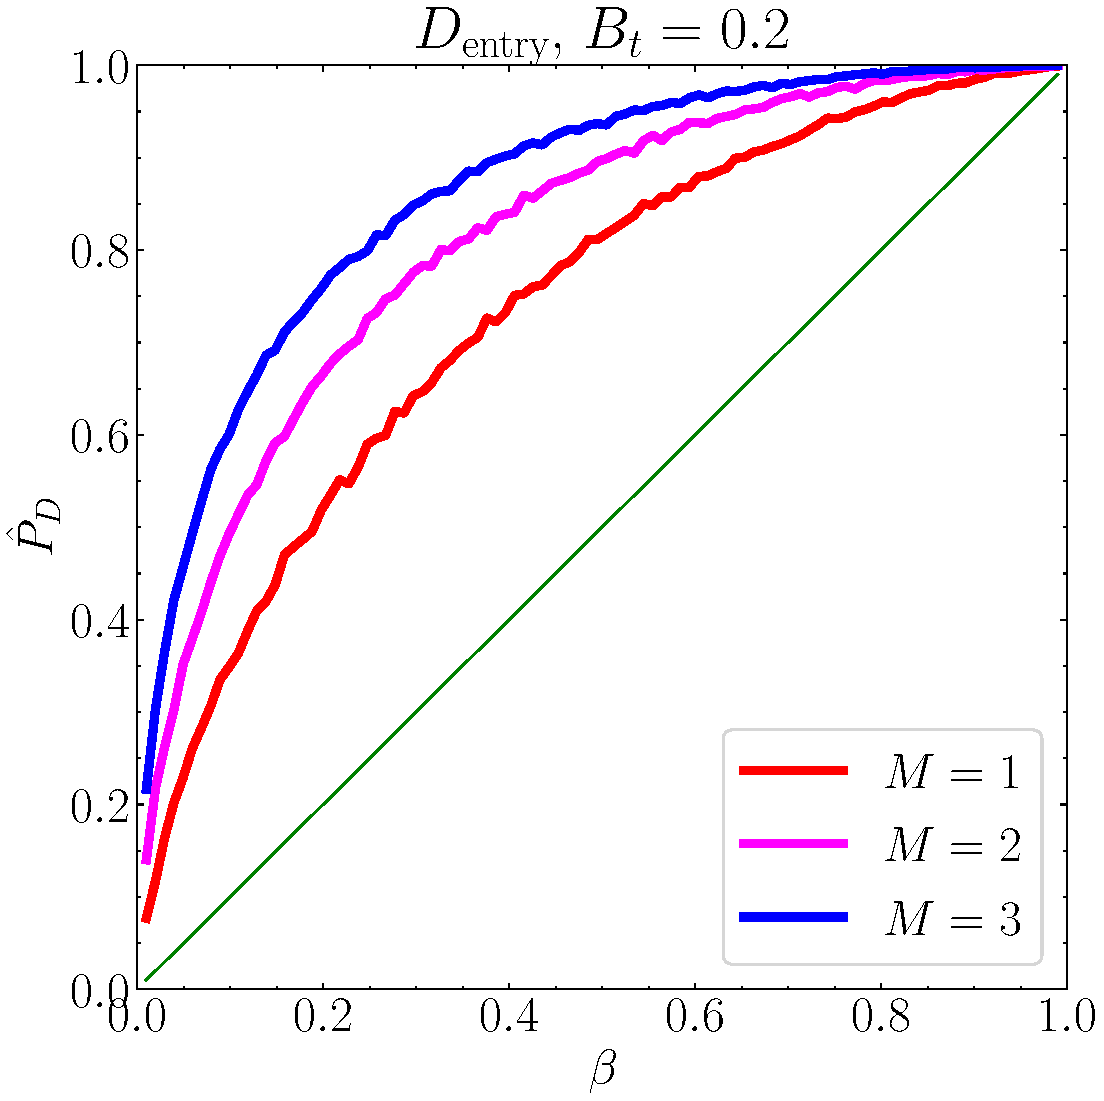
\includegraphics[width=2in]{../results/CDR/CDR_PD_Bt_0.2}}
\subfigure[$B_{t}=0.3$]{\label{fig:a}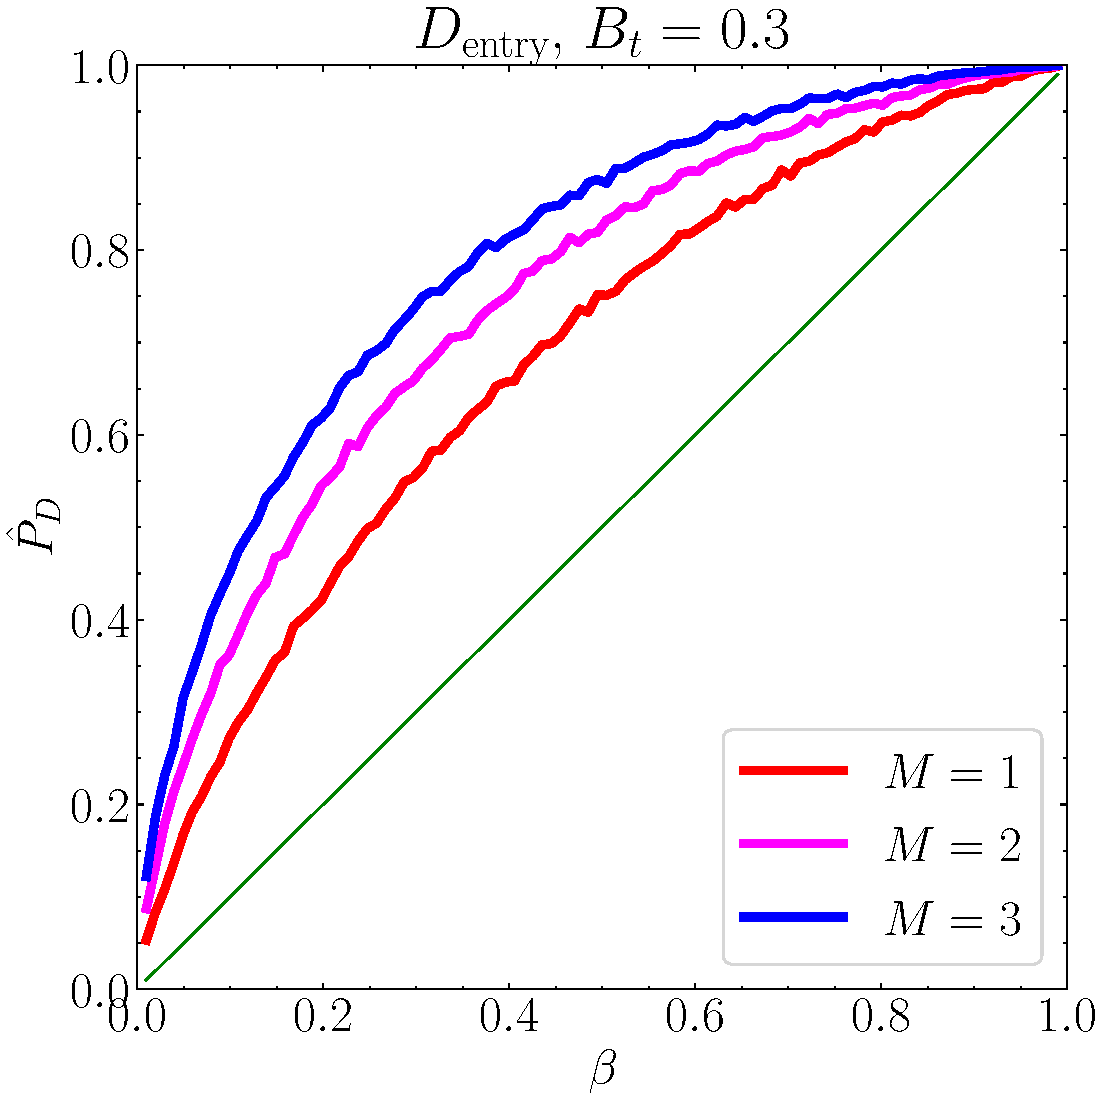
\includegraphics[width=2in]{../results/CDR/CDR_PD_Bt_0.3}}
\subfigure[$B_{t}=0.4$]{\label{fig:a}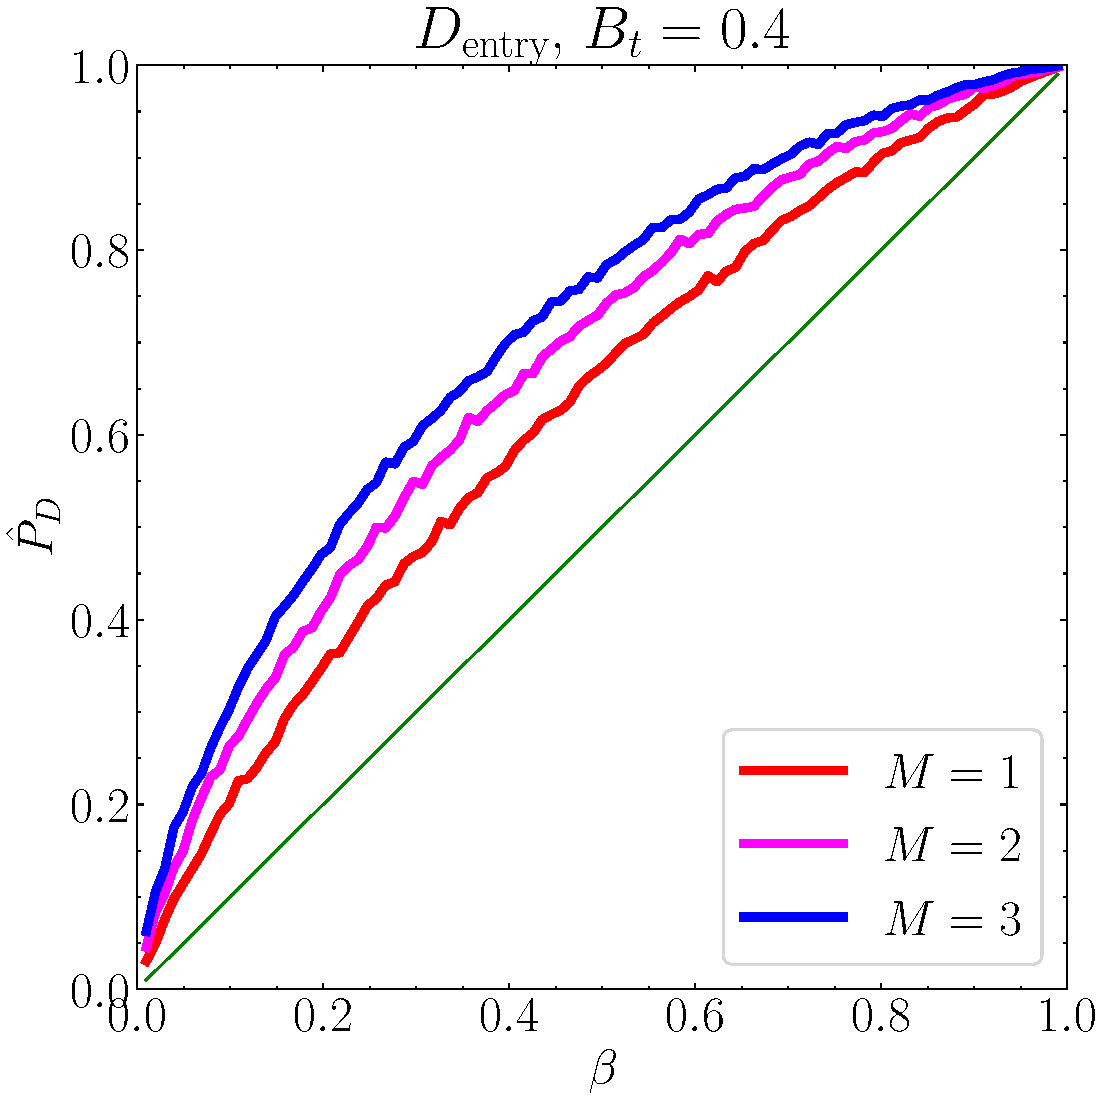
\includegraphics[width=2in]{../results/CDR/CDR_PD_Bt_0.4}}
\subfigure[$B_{t}=0.5$]{\label{fig:a}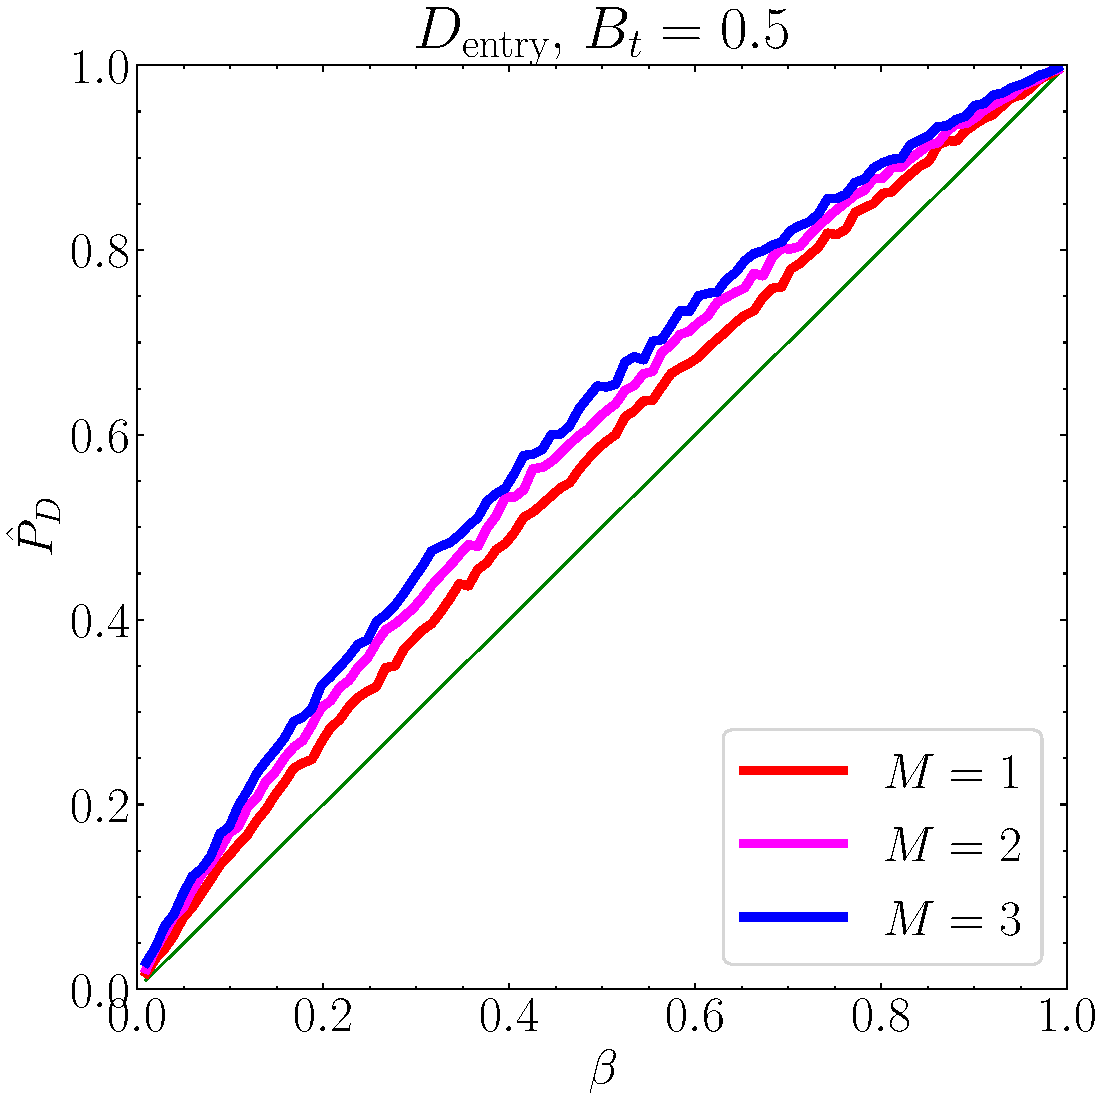
\includegraphics[width=2in]{../results/CDR/CDR_PD_Bt_0.5}}
\subfigure[$B_{t}=0.6$]{\label{fig:a}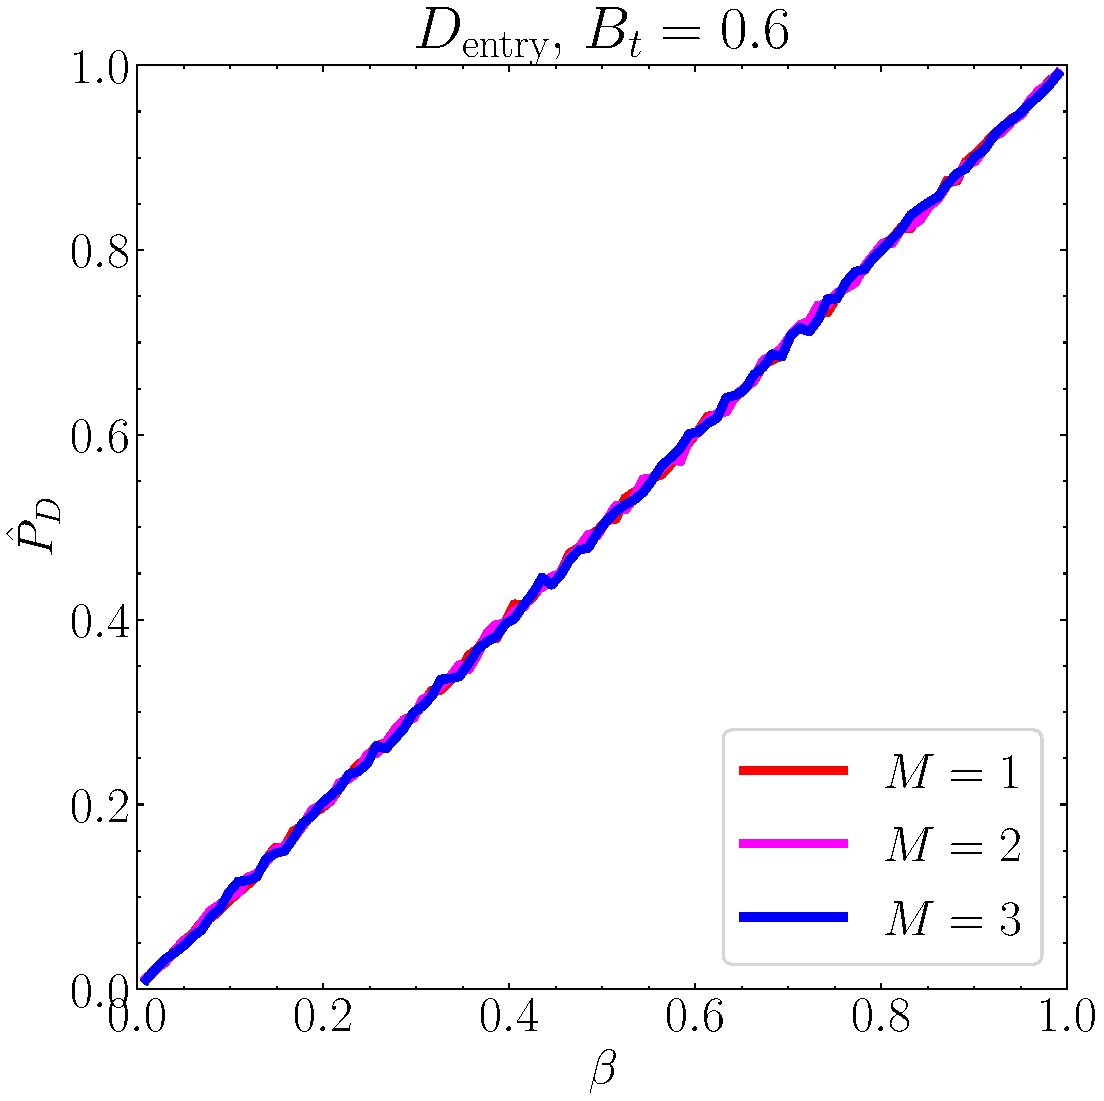
\includegraphics[width=2in]{../results/CDR/CDR_PD_Bt_0.6}}
\caption{[Colour online] Variation of estimated probability of detection with varying bounds $\beta$ and number of channels $M$, for each value of parameter $B_{t}$. The green line shows the equality constraint $P_{D}=\beta$.}
\label{fig:MCdentry}
\end{figure}

Figure \ref{fig:MCdentry} shows the variation of the estimated probability of detection $\hat{P}_{D}$ with the bound $\beta$. We observe, in all cases, the probability of detection is bounded below by the parameter $\beta$. Since the parameter matches the true value for $B_{t}=0.6$, we see that $\hat{P}_{D}=\beta$, and for values of $B_{t}$ diverging from $0.6$, the estimated probability of detection moves further away from the bound. For any fixed value of $B_{t}$, and fixed value of $\beta$, we observe the estimated probability of detection increases with the increase in the number of channels $M$. This is as expected using the law of large numbers.

% -----------------------------------------------------------------------------------------------------------------------

\subsubsection{ROC of $D_{\text{entry}}$}
\label{subsubsec:entryDetector_roc}

Using the Monte-Carlo simulations in Section \ref{subsubsec:entryDetector_working}, we plot the ROC for $D_{\text{entry}}$, for each of the six values of $B_{t}$ considered. We also compare it to the true ROC using (\ref{eq:CDRpfa}).
\begin{figure}[h!]
\centering
\subfigure[$B_{t}=0.1$]{\label{fig:a}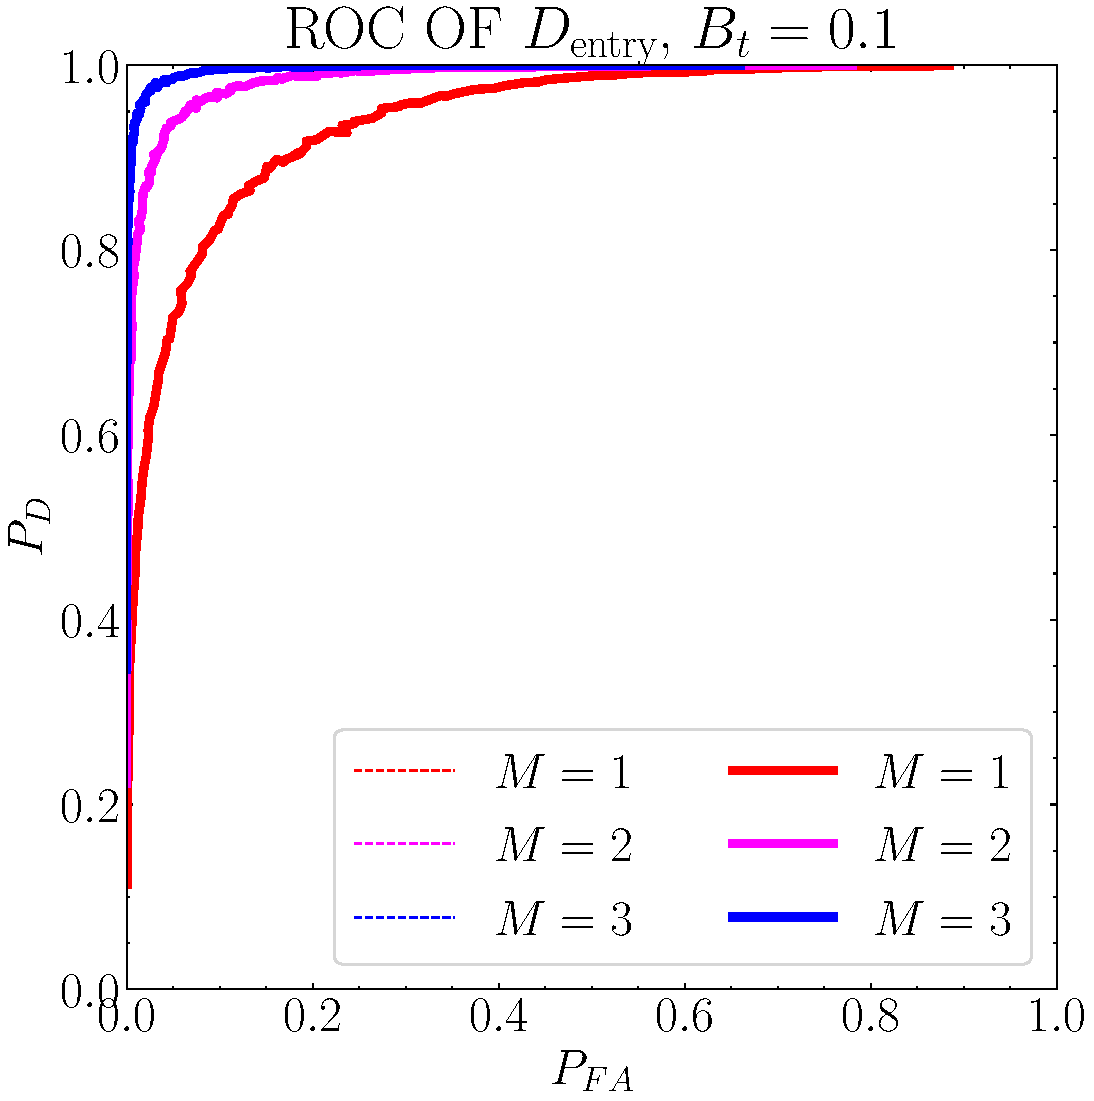
\includegraphics[width=2in]{../results/CDR/CDR_ROC_Bt_0.1}}
\subfigure[$B_{t}=0.2$]{\label{fig:a}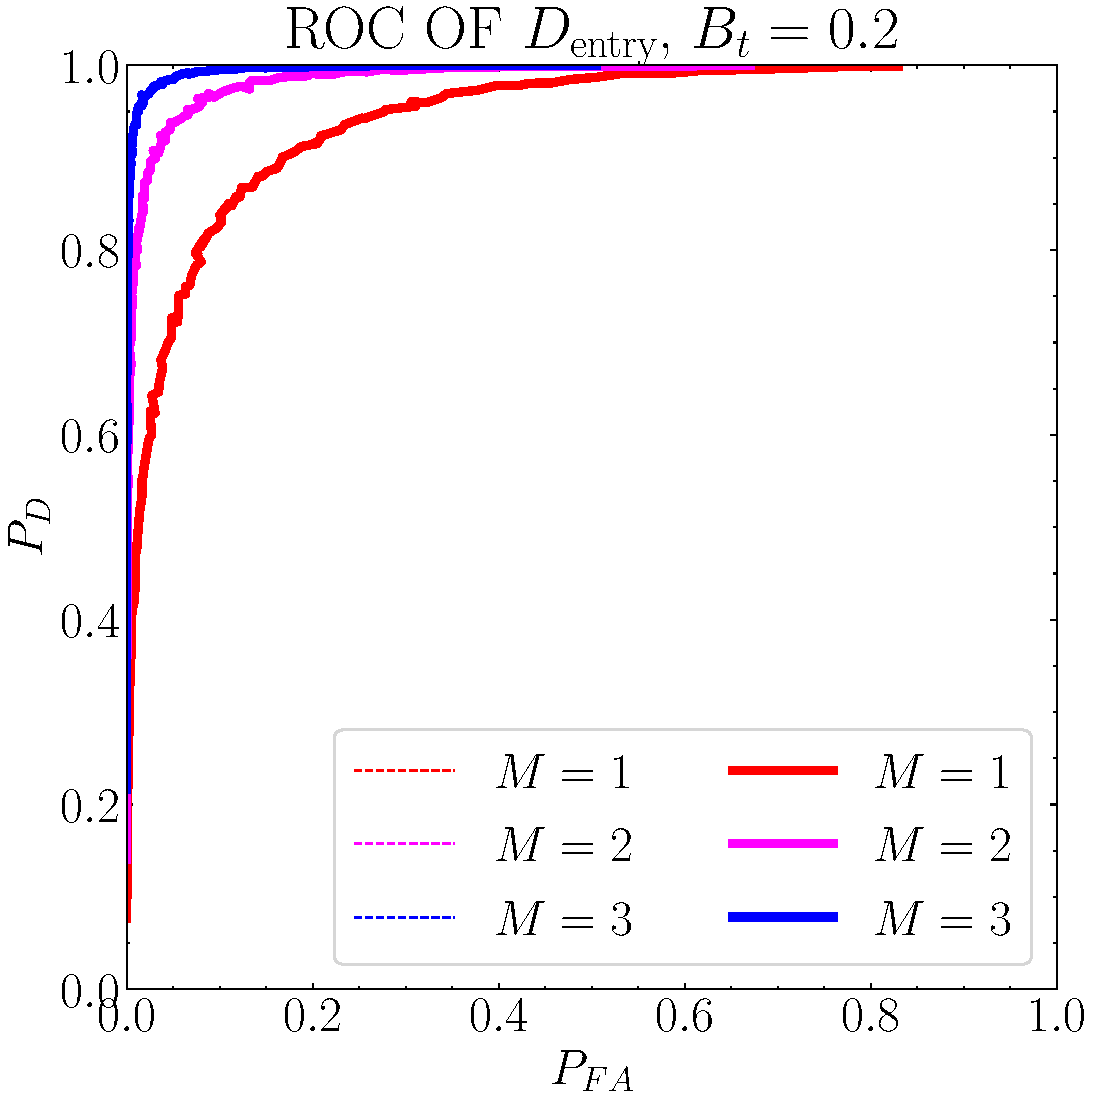
\includegraphics[width=2in]{../results/CDR/CDR_ROC_Bt_0.2}}
\subfigure[$B_{t}=0.3$]{\label{fig:a}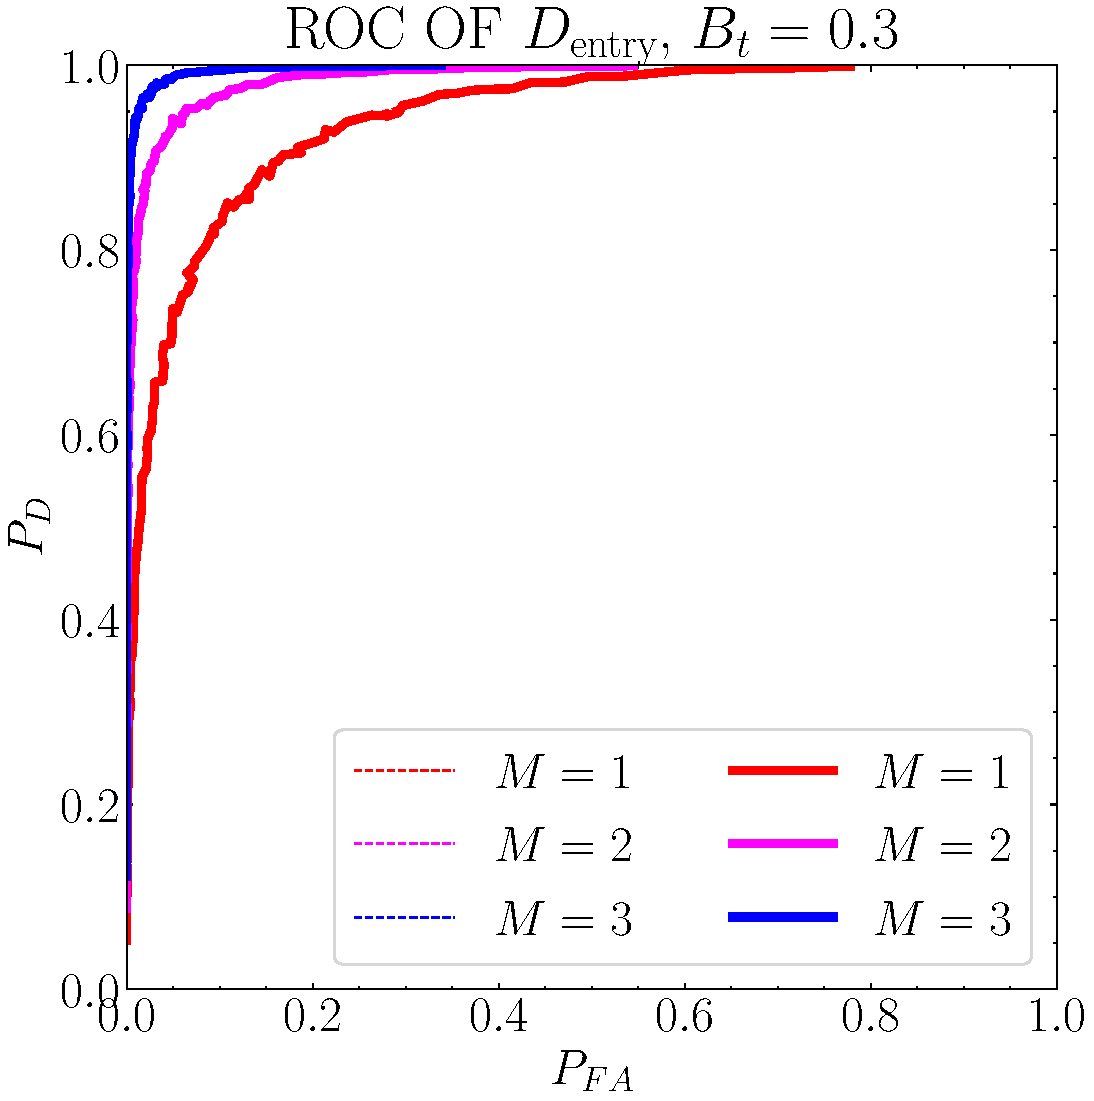
\includegraphics[width=2in]{../results/CDR/CDR_ROC_Bt_0.3}}
\subfigure[$B_{t}=0.4$]{\label{fig:a}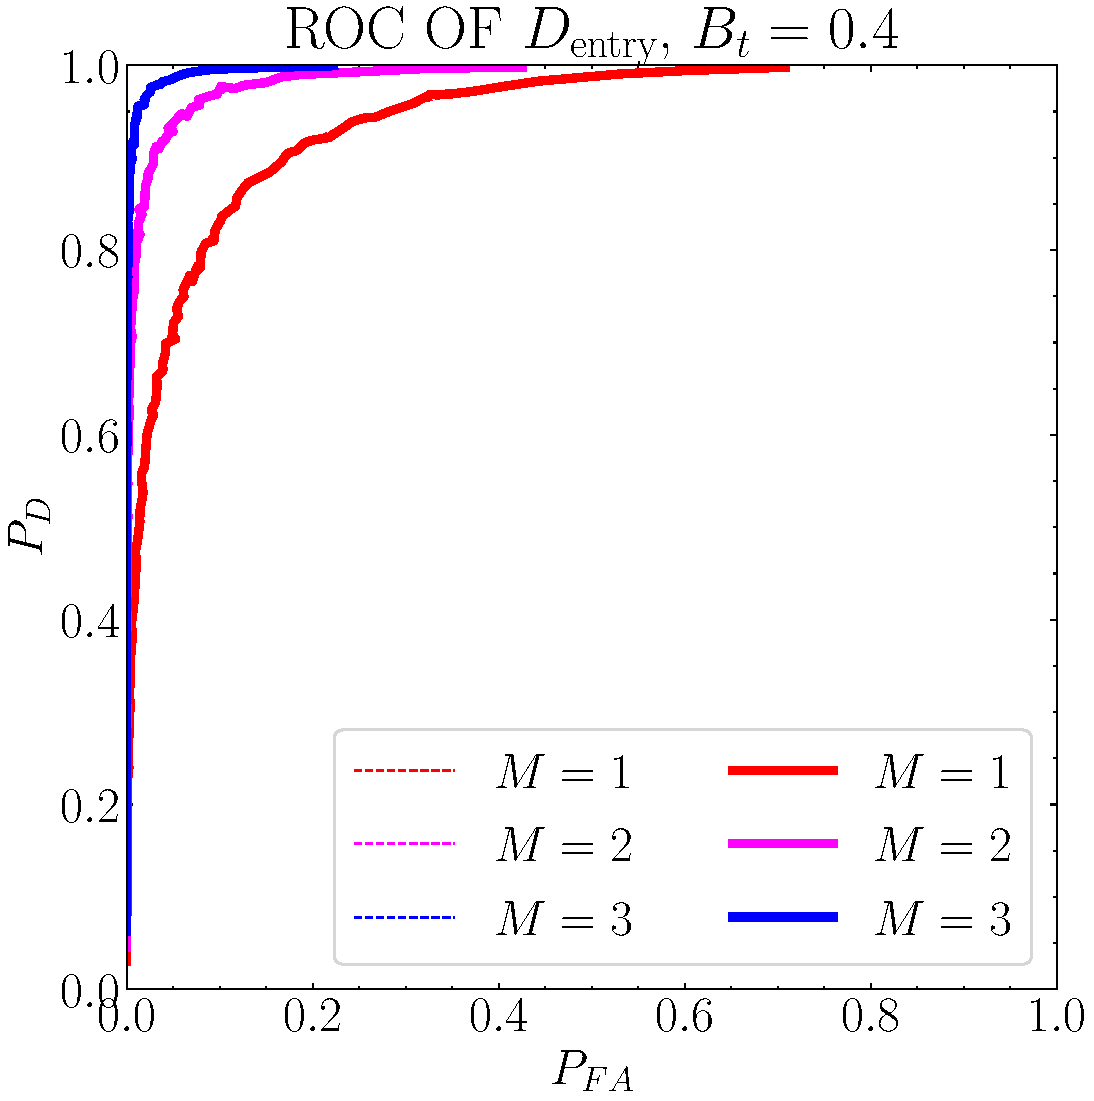
\includegraphics[width=2in]{../results/CDR/CDR_ROC_Bt_0.4}}
\subfigure[$B_{t}=0.5$]{\label{fig:a}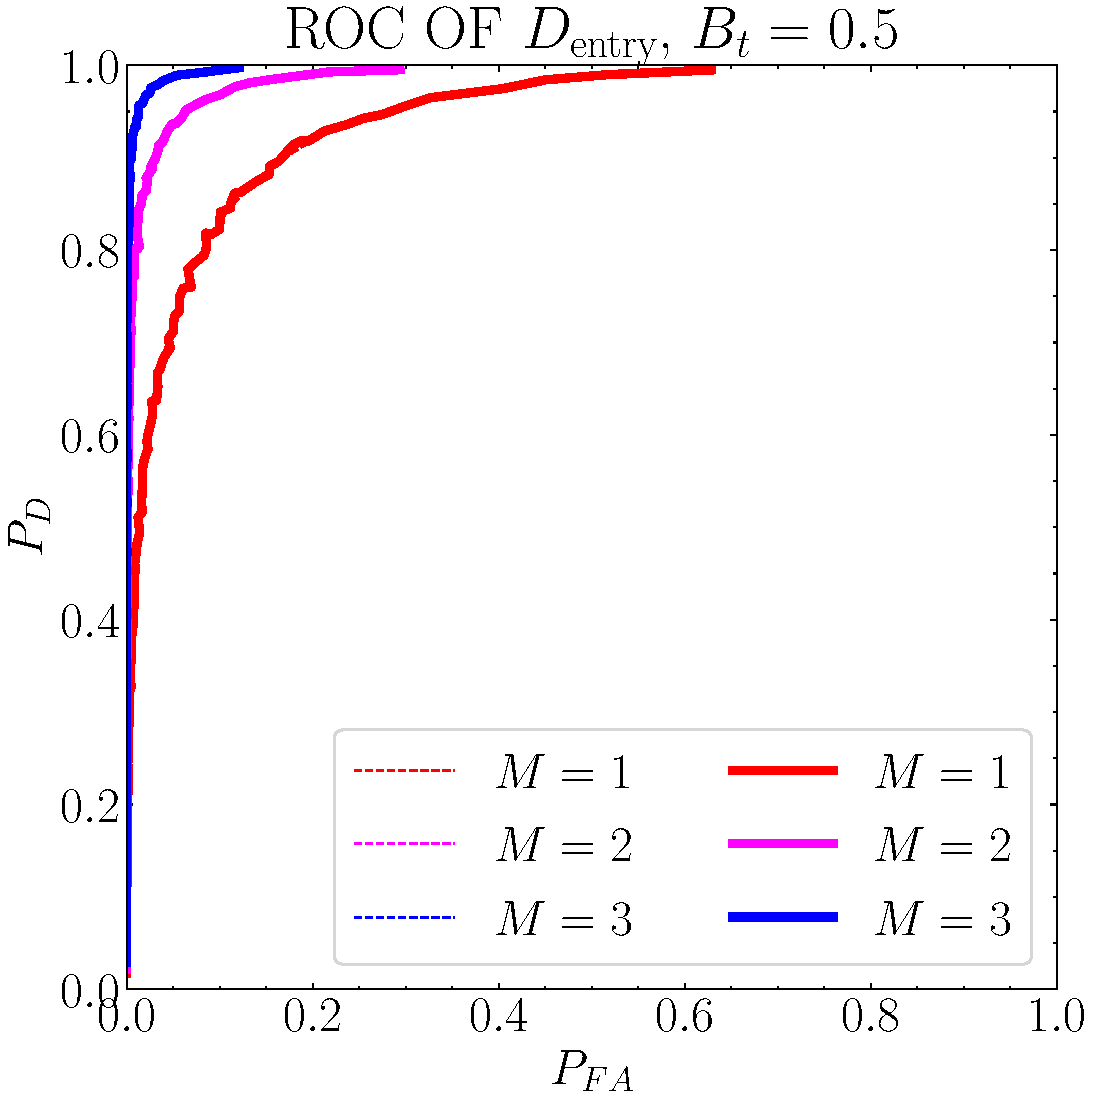
\includegraphics[width=2in]{../results/CDR/CDR_ROC_Bt_0.5}}
\subfigure[$B_{t}=0.6$]{\label{fig:a}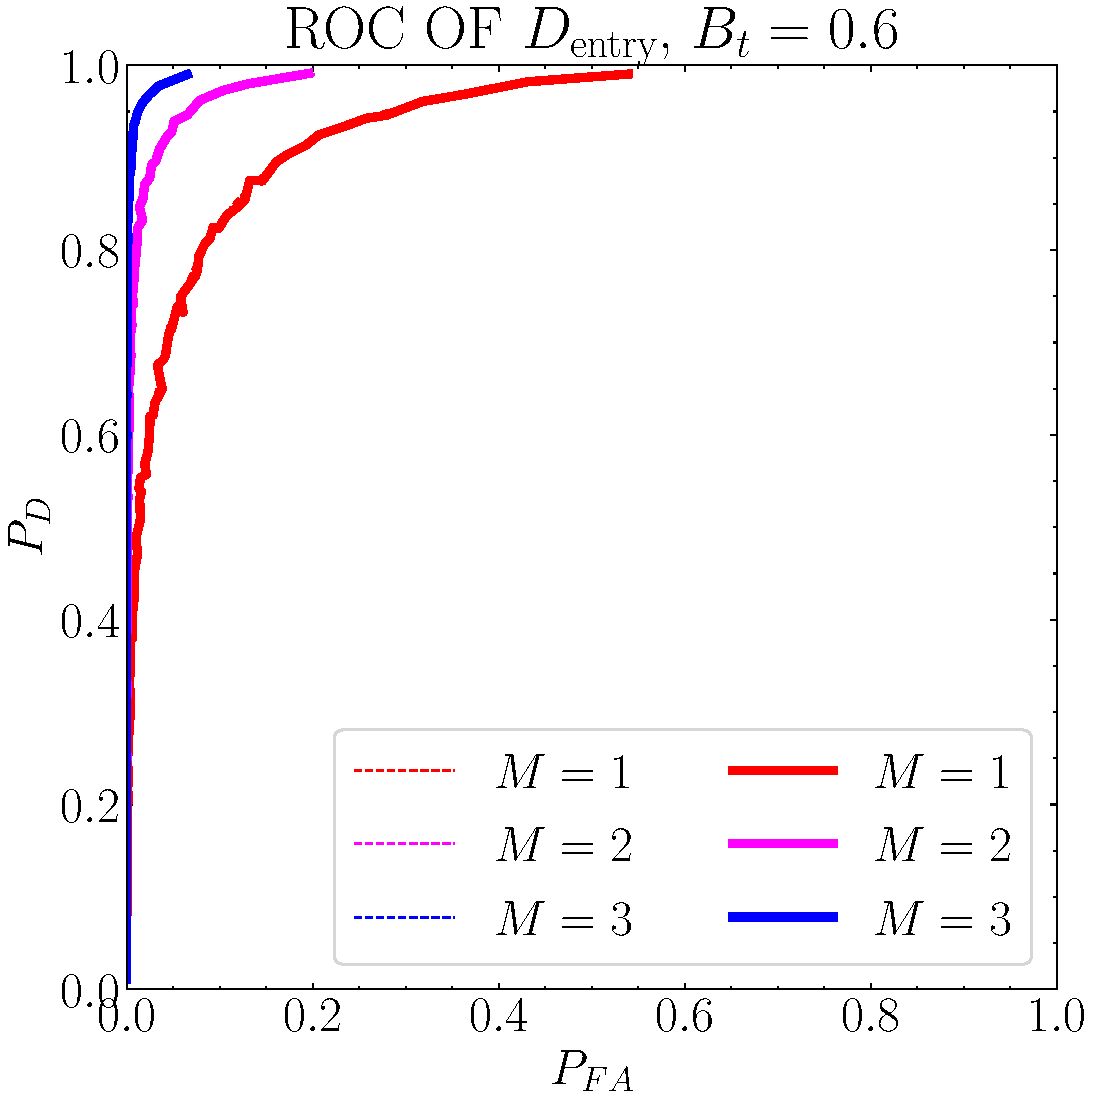
\includegraphics[width=2in]{../results/CDR/CDR_ROC_Bt_0.6}}
\caption{[Colour online] ROC for the detector for varying number of channels $M$, for each value of parameter $B_{t}$. Solid lines show the estimated ROC and dashed lines show the theoretical ROC.}
\label{fig:ROCdentry}
\end{figure}

Figure \ref{fig:ROCdentry} shows the ROC for $D_{\text{entry}}$ with varying number of channels $M$, and for each value of $B_{t}$. We observe that the ROC is identical for each setting $M$, over varying $B_{t}$. This shows that the detector is independent of $B_{t}$, as designed. For any given value of $B_{t}$, we observe the ROC is concave, i.e., achieves high probability of detection for low probability of false alarm, and matches the theoretical ROC, in all cases with varying $M$. Between the ROC for varying $M$, we see that the ROC with a larger value for $M$ is more concave. This is, again, as expected as more channels implies more measurements.

% -----------------------------------------------------------------------------------------------------------------------

\subsubsection{Monte-Carlo simulations for $D_{\text{exit}}$}
\label{subsubsec:exitDetector_working}

We implement $D_{\text{exit}}$ using the threshold (\ref{eq:generalCFARthreshold}), and perform Monte-Carlo simulations averaged over $10000$ realisations to estimate the probability of false alarm $\hat{P}_{FA}$. We repeat the experiment for the six values of $B_{t}$ considered and vary $M=1,2,3$ in each case.
\begin{figure}[h!]
\centering
\subfigure[$B_{t}=0.1$]{\label{fig:a}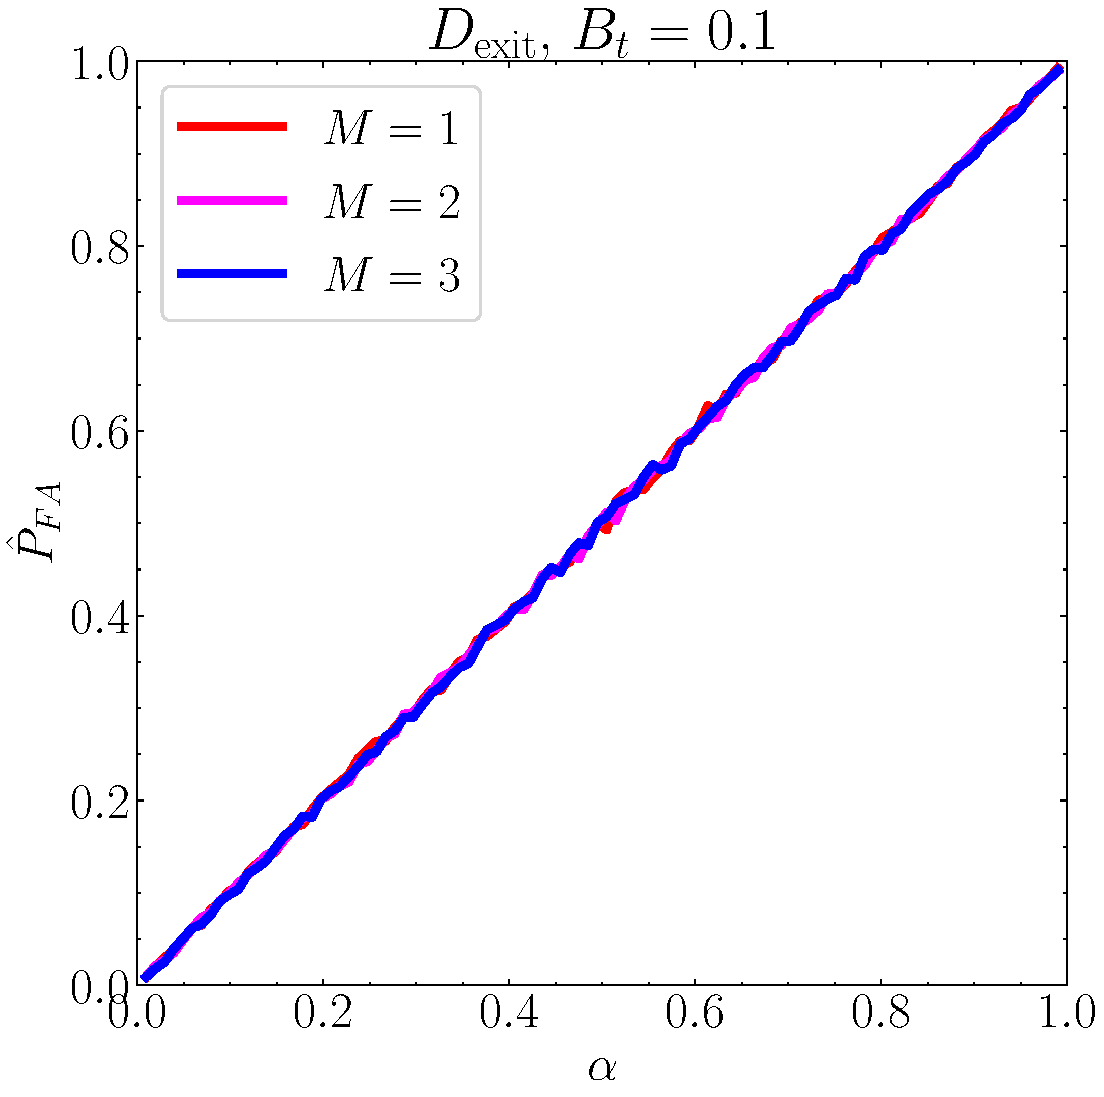
\includegraphics[width=2in]{../results/CFAR/CFAR_PFA_Bt_0.1}}
\subfigure[$B_{t}=0.2$]{\label{fig:a}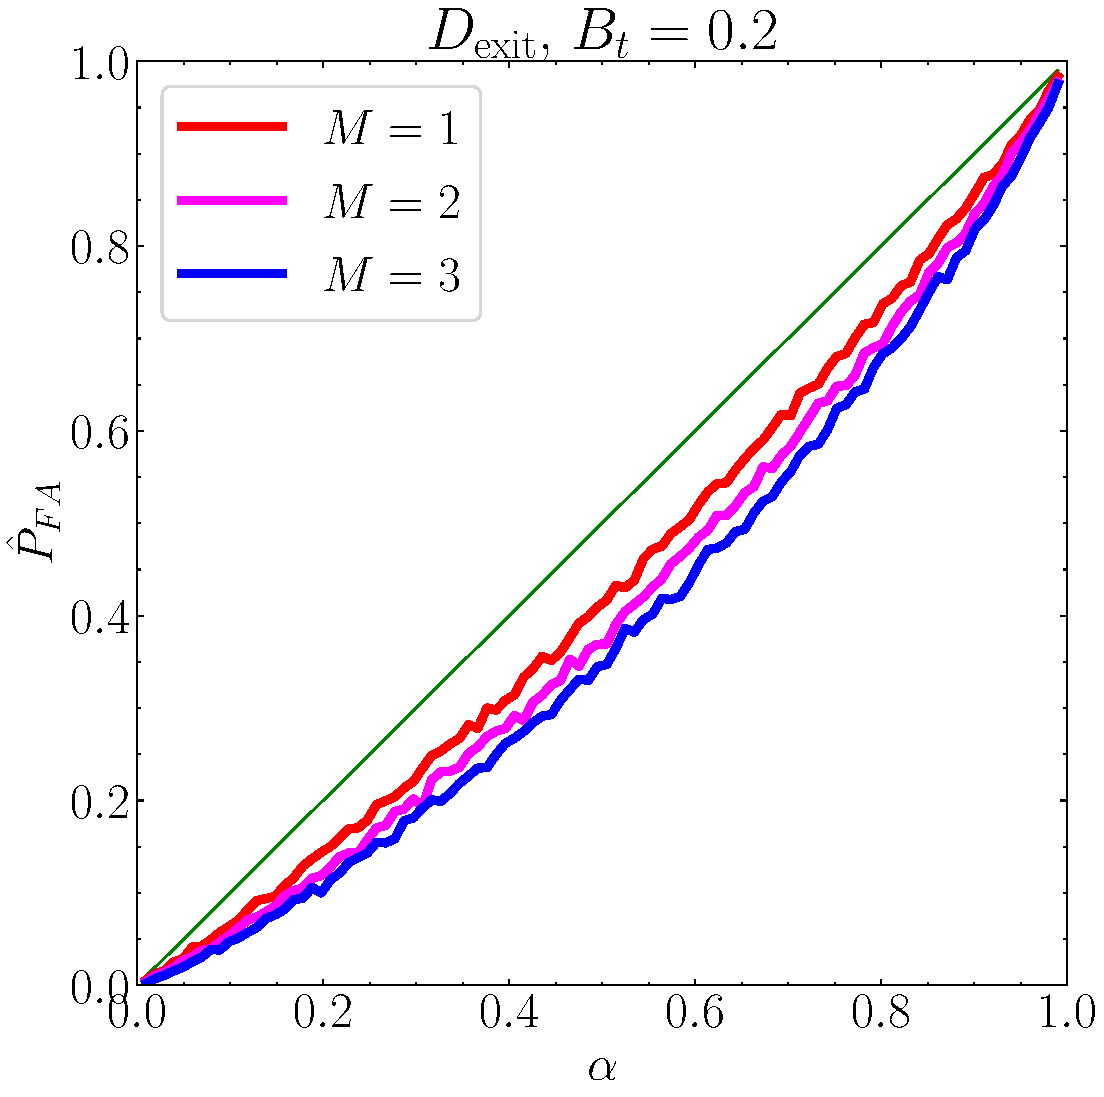
\includegraphics[width=2in]{../results/CFAR/CFAR_PFA_Bt_0.2}}
\subfigure[$B_{t}=0.3$]{\label{fig:a}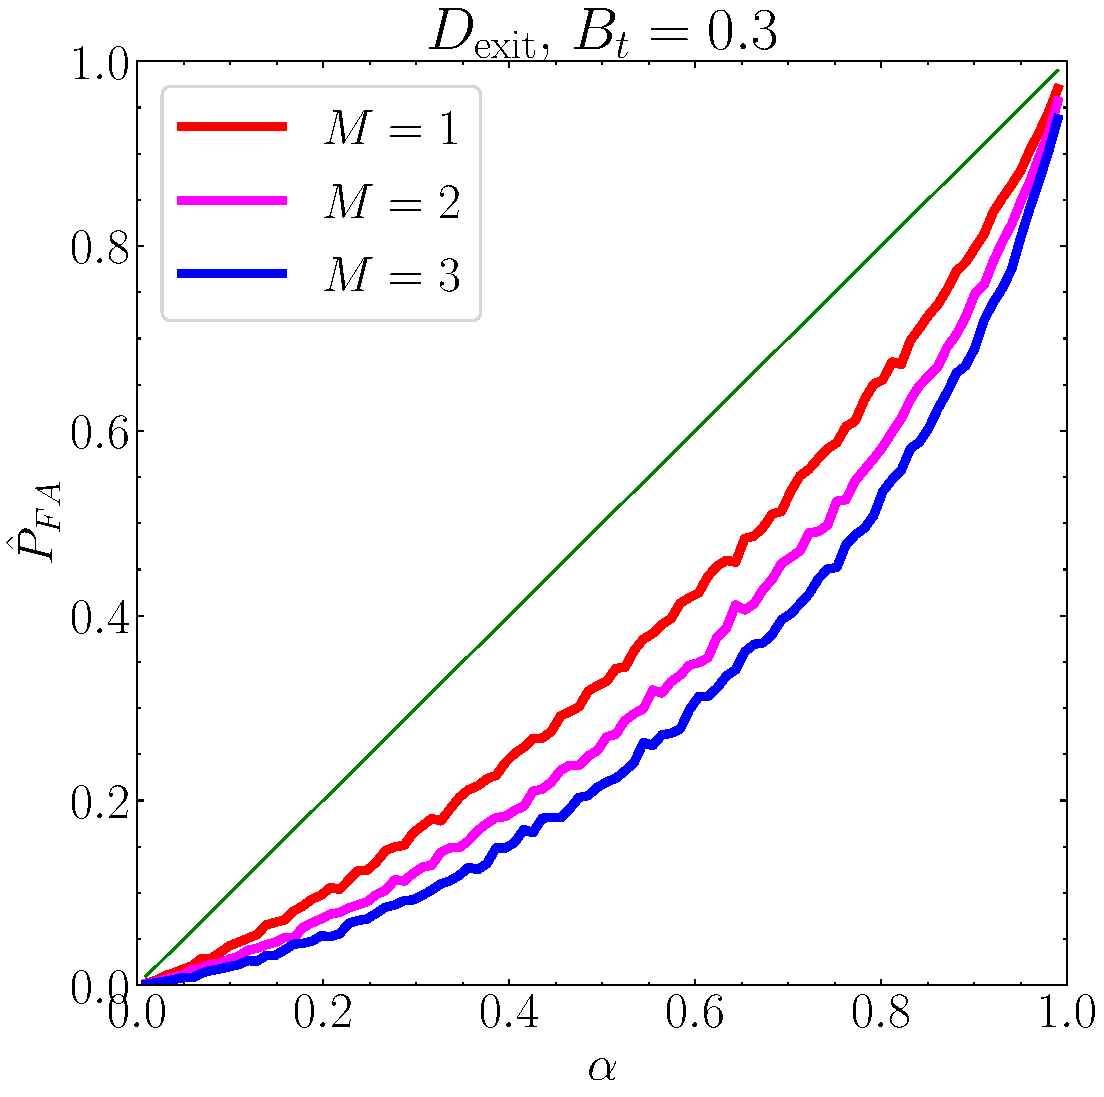
\includegraphics[width=2in]{../results/CFAR/CFAR_PFA_Bt_0.3}}
\subfigure[$B_{t}=0.4$]{\label{fig:a}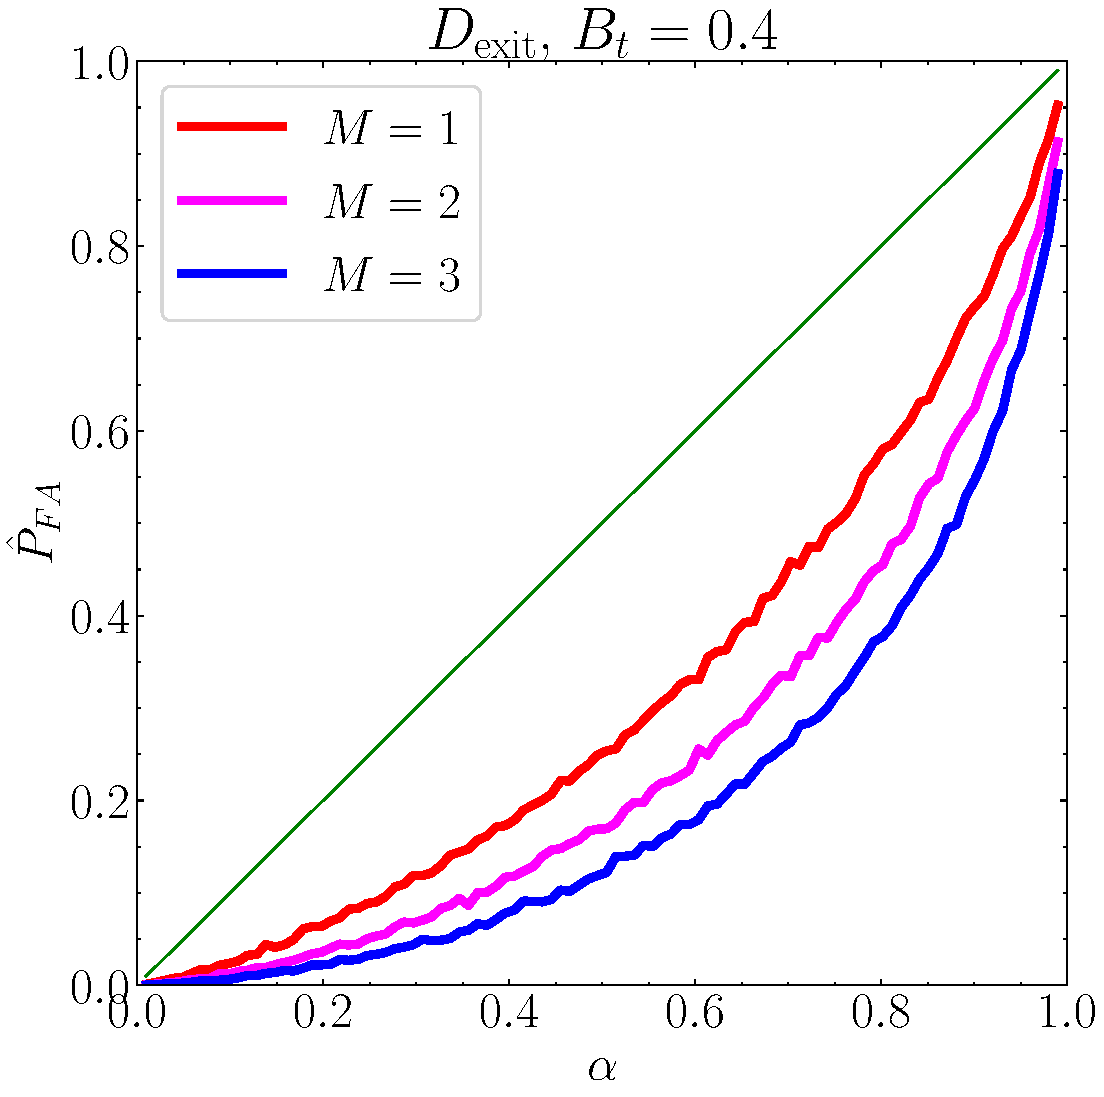
\includegraphics[width=2in]{../results/CFAR/CFAR_PFA_Bt_0.4}}
\subfigure[$B_{t}=0.5$]{\label{fig:a}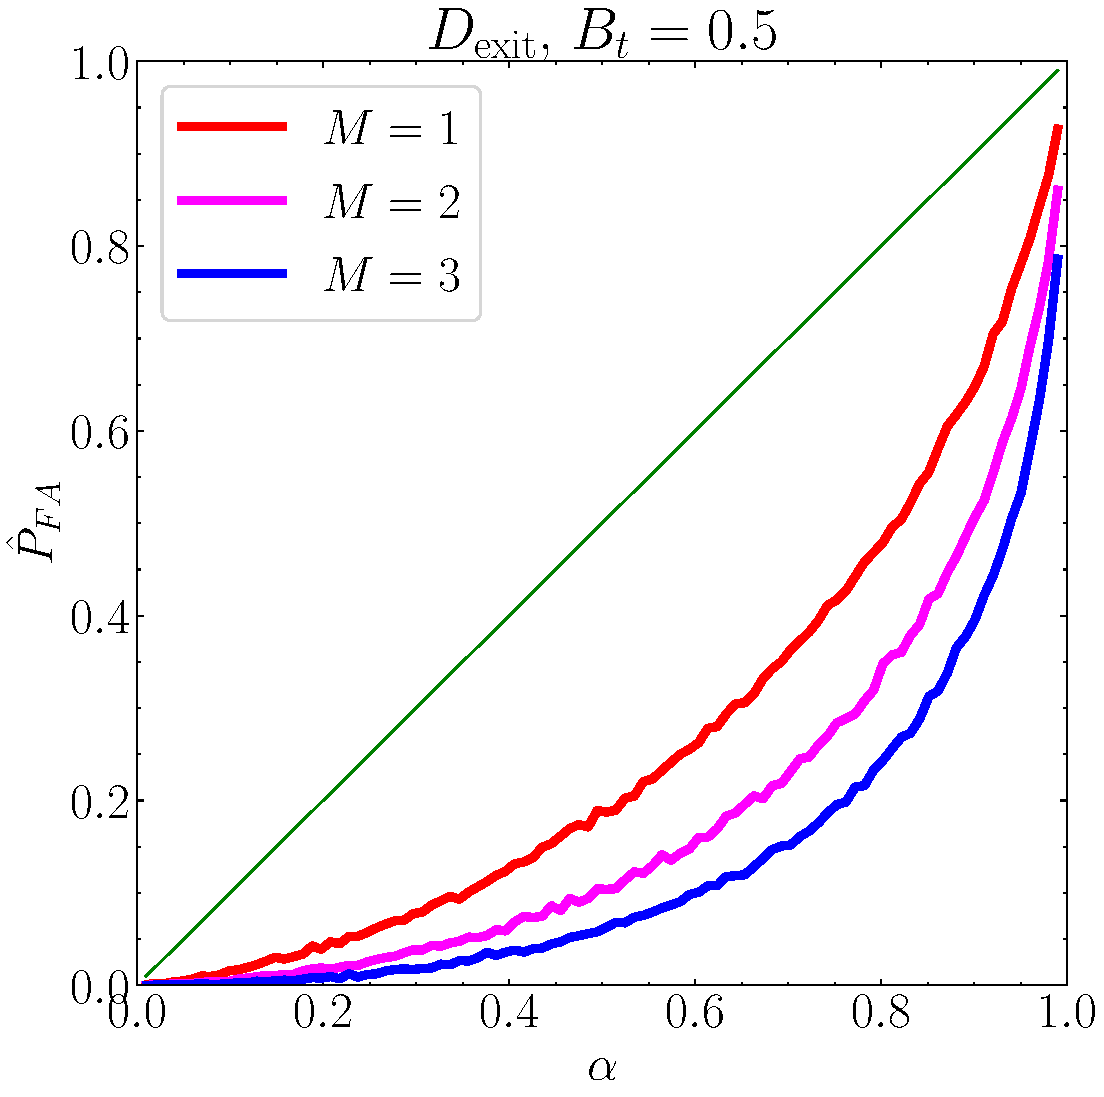
\includegraphics[width=2in]{../results/CFAR/CFAR_PFA_Bt_0.5}}
\subfigure[$B_{t}=0.6$]{\label{fig:a}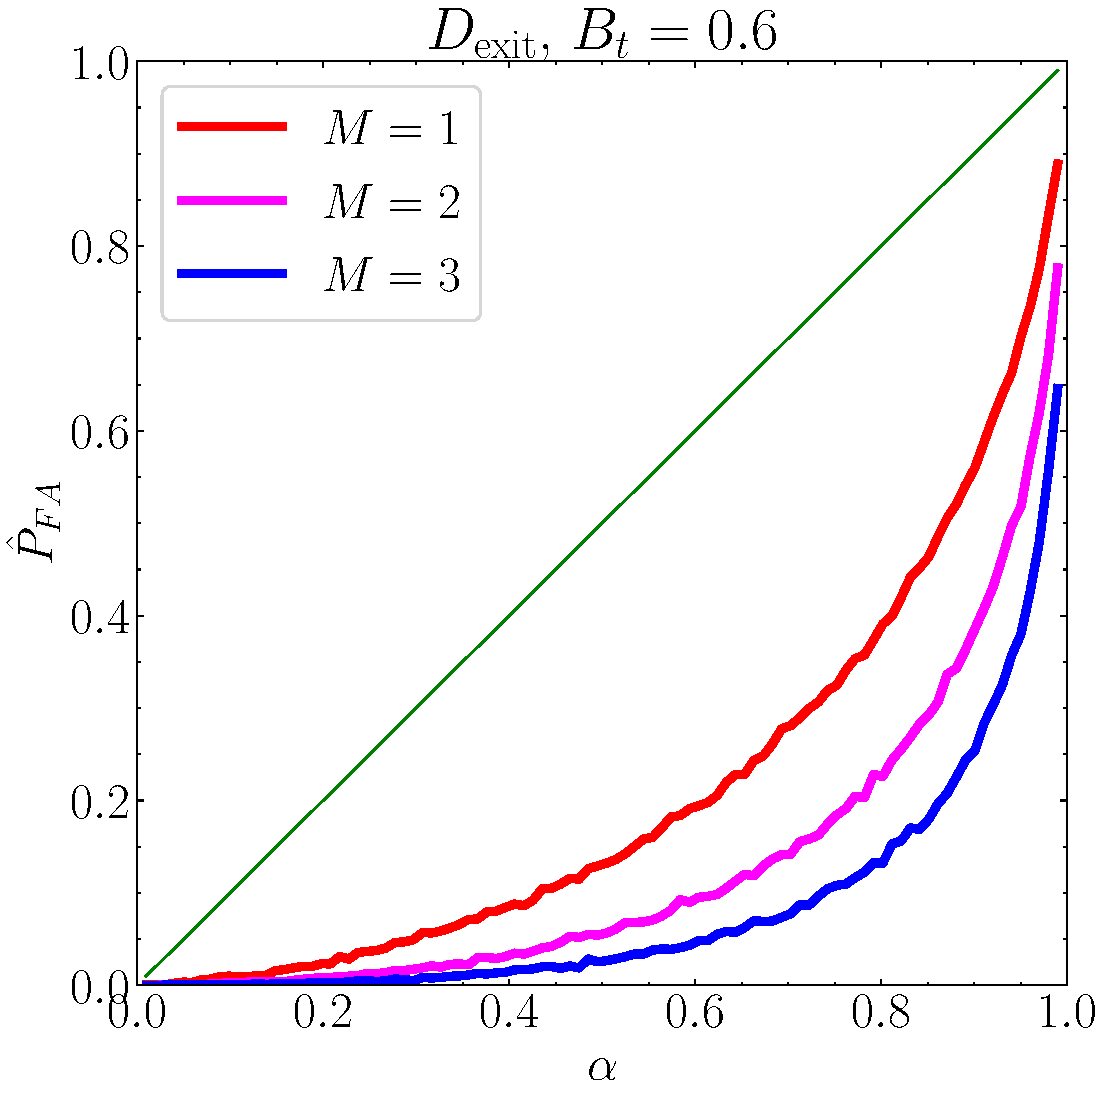
\includegraphics[width=2in]{../results/CFAR/CFAR_PFA_Bt_0.6}}
\caption{[Colour online] Variation of estimated probability of false alarm with varying bounds $\alpha$ and number of channels $M$, for each value of parameter $B_{t}$.}
\label{fig:MCdexit}
\end{figure}

Figure \ref{fig:MCdexit} shows the variation of the estimated probability of false alarm $\hat{P}_{FA}$ with the bound $\alpha$. We observe, in all cases, the probability of false alarm is bounded above by the parameter $\alpha$. Since the parameter matches the true value for $B_{t}=0.1$, we see that $\hat{P}_{FA}=\alpha$, and for values of $B_{t}$ diverging from $0.1$, the estimated probability of false alarm moves further away from the bound. For any fixed value of $B_{t}$, and fixed value of $\alpha$, we observe the estimated probability of false alarm decreases with the increase in the number of channels $M$. This is as expected using the law of large numbers.

% -----------------------------------------------------------------------------------------------------------------------

\subsubsection{ROC of $D_{\text{exit}}$}
\label{subsubsec:exitDetector_roc}

Using the Monte-Carlo simulations in Section \ref{subsubsec:exitDetector_working}, we plot the ROC for $D_{\text{exit}}$, for each of the six values of $B_{t}$ considered. We also compare it to the true ROC using (\ref{eq:CFARpd}).
\begin{figure}[h!]
\centering
\subfigure[$B_{t}=0.1$]{\label{fig:a}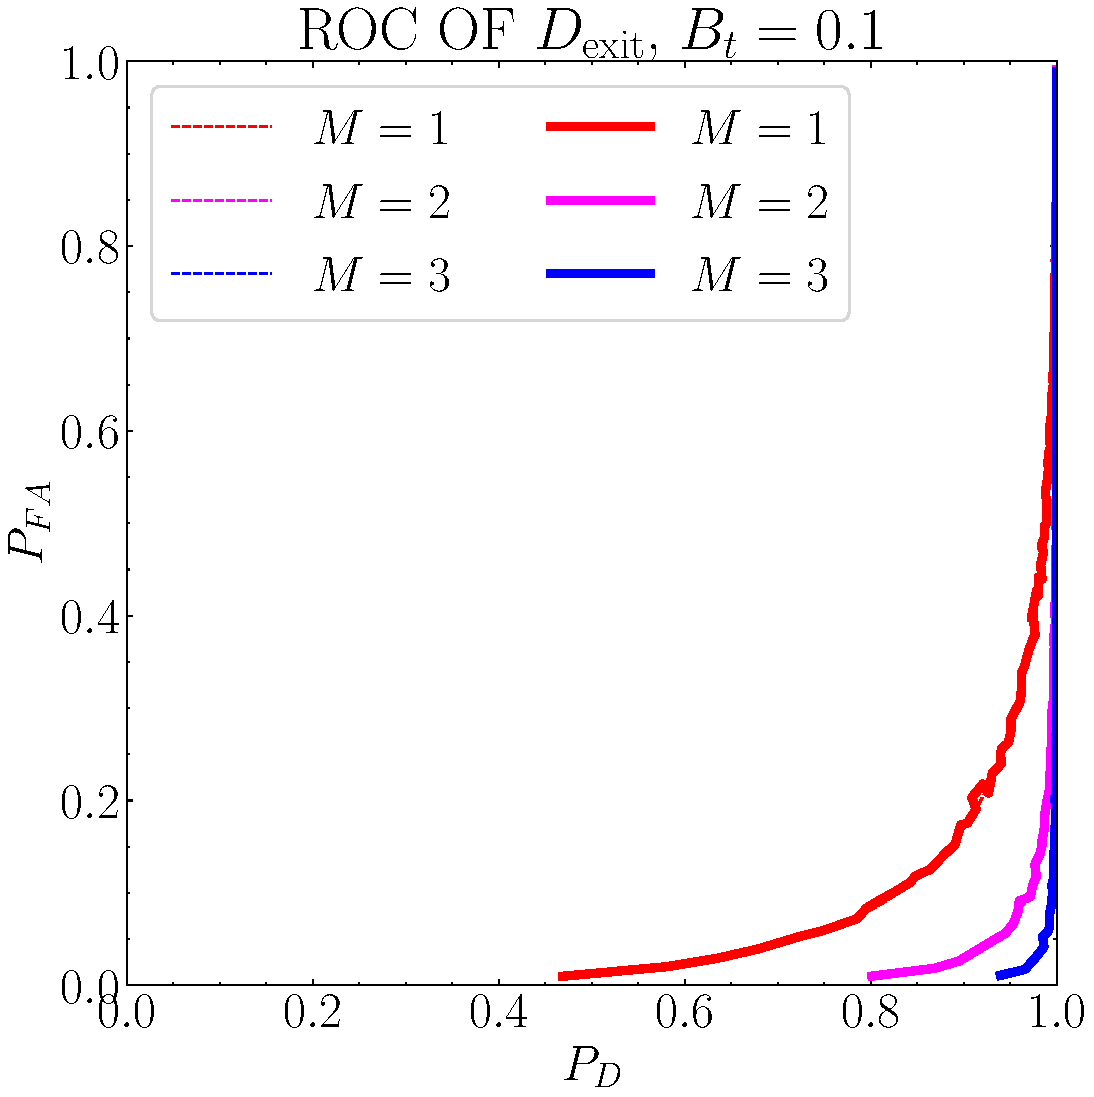
\includegraphics[width=2in]{../results/CFAR/CFAR_ROC_Bt_0.1}}
\subfigure[$B_{t}=0.2$]{\label{fig:a}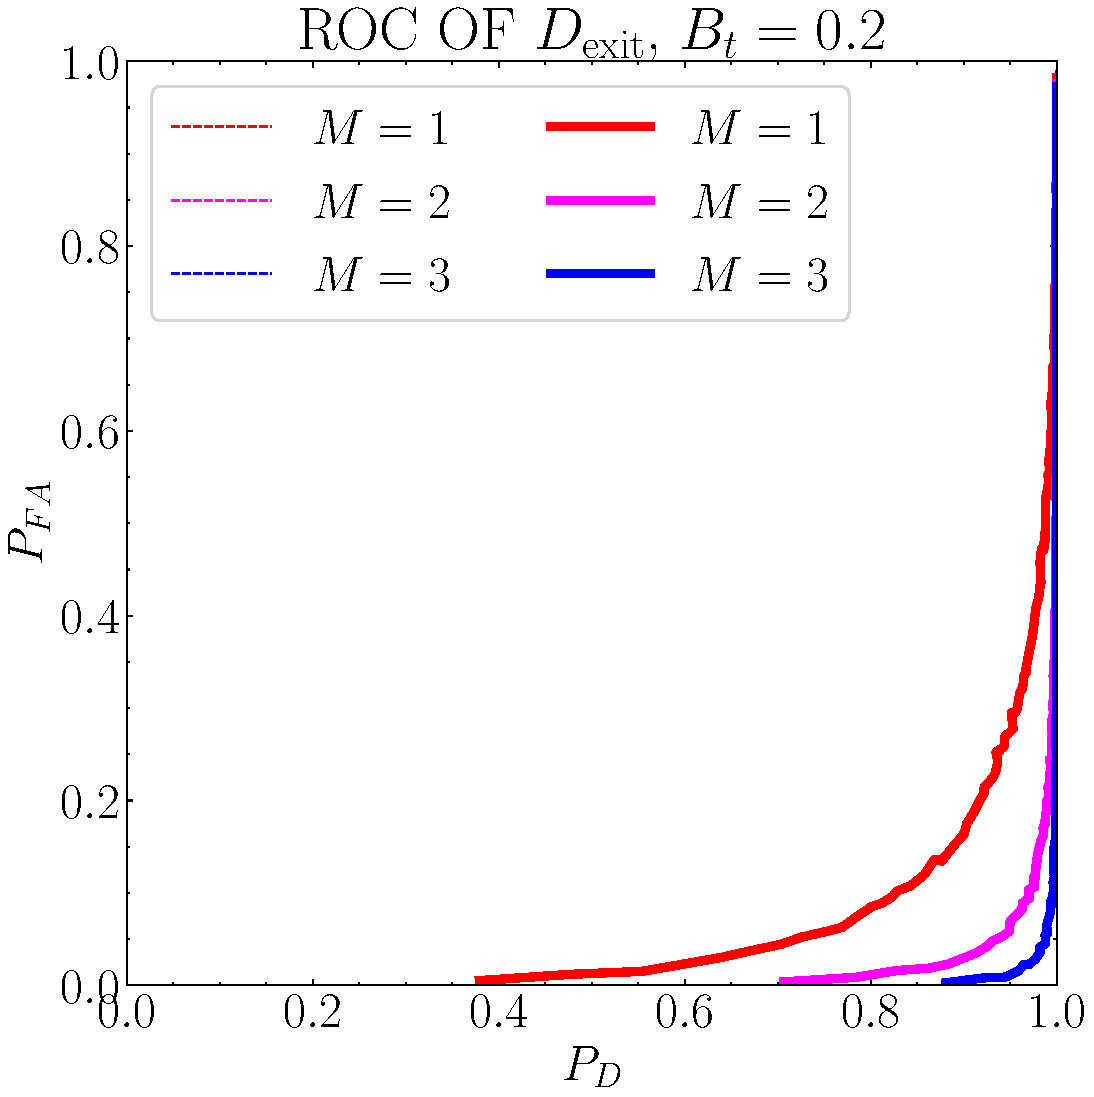
\includegraphics[width=2in]{../results/CFAR/CFAR_ROC_Bt_0.2}}
\subfigure[$B_{t}=0.3$]{\label{fig:a}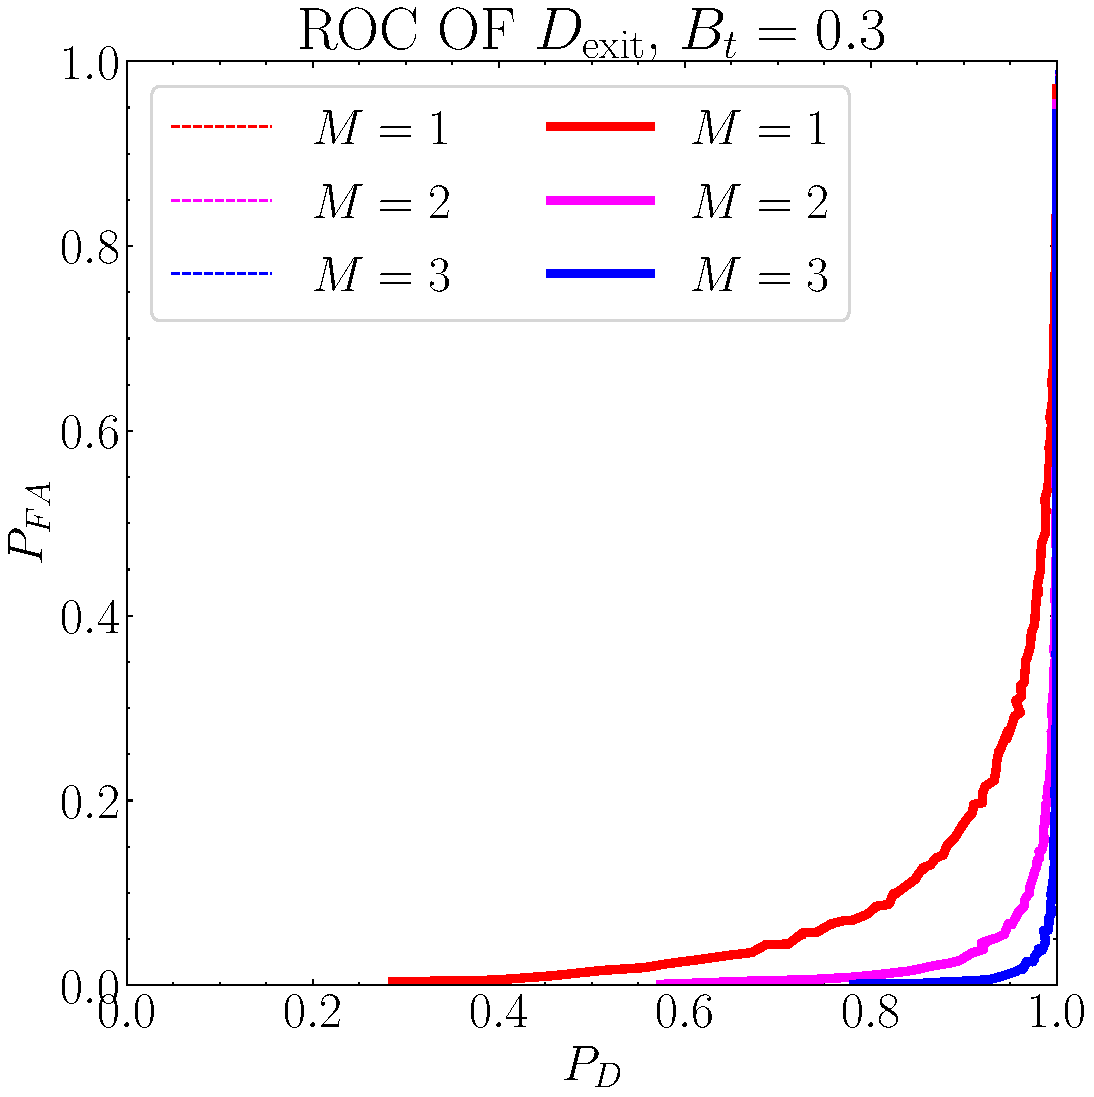
\includegraphics[width=2in]{../results/CFAR/CFAR_ROC_Bt_0.3}}
\subfigure[$B_{t}=0.4$]{\label{fig:a}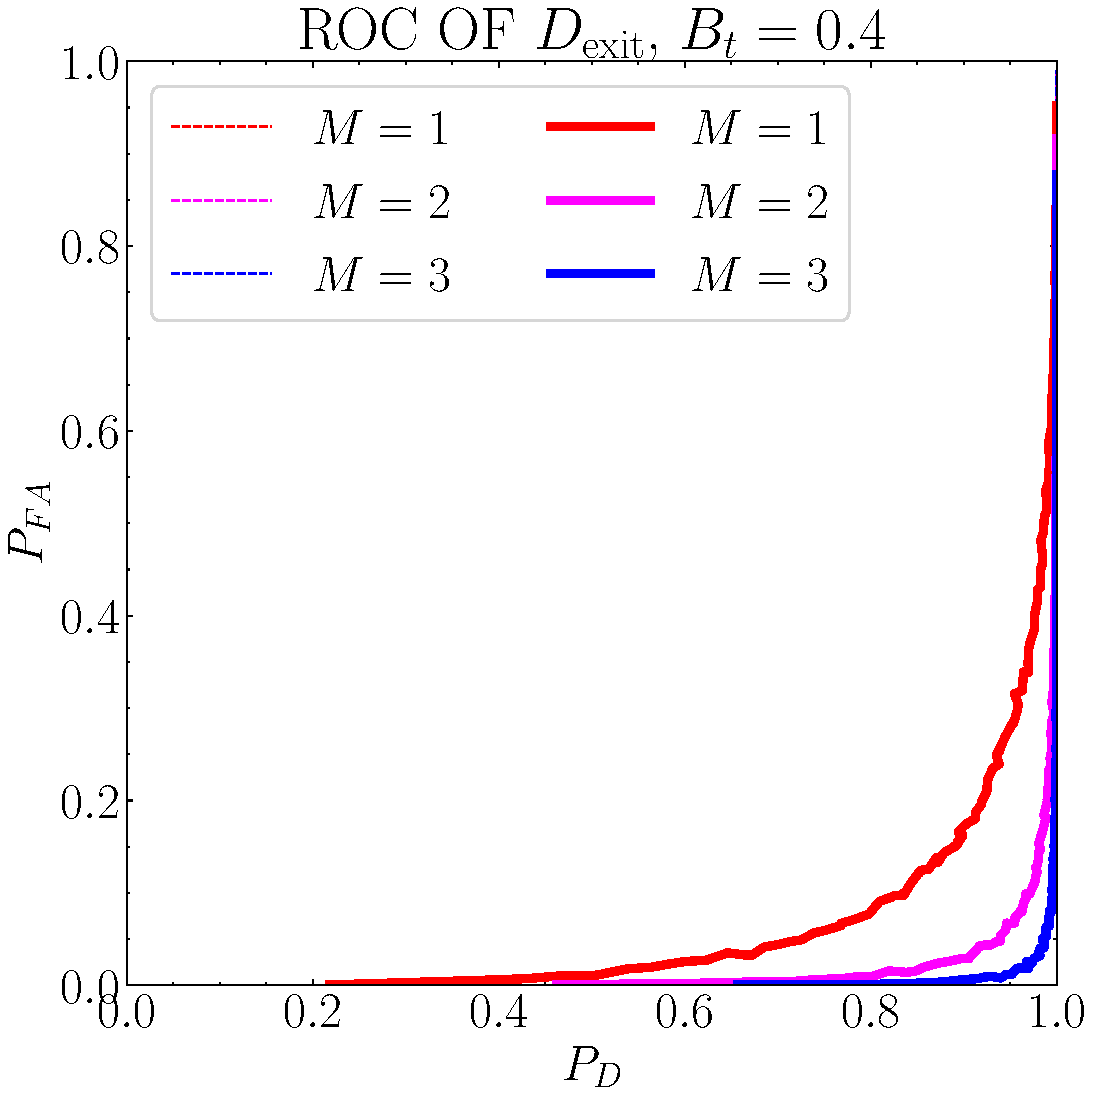
\includegraphics[width=2in]{../results/CFAR/CFAR_ROC_Bt_0.4}}
\subfigure[$B_{t}=0.5$]{\label{fig:a}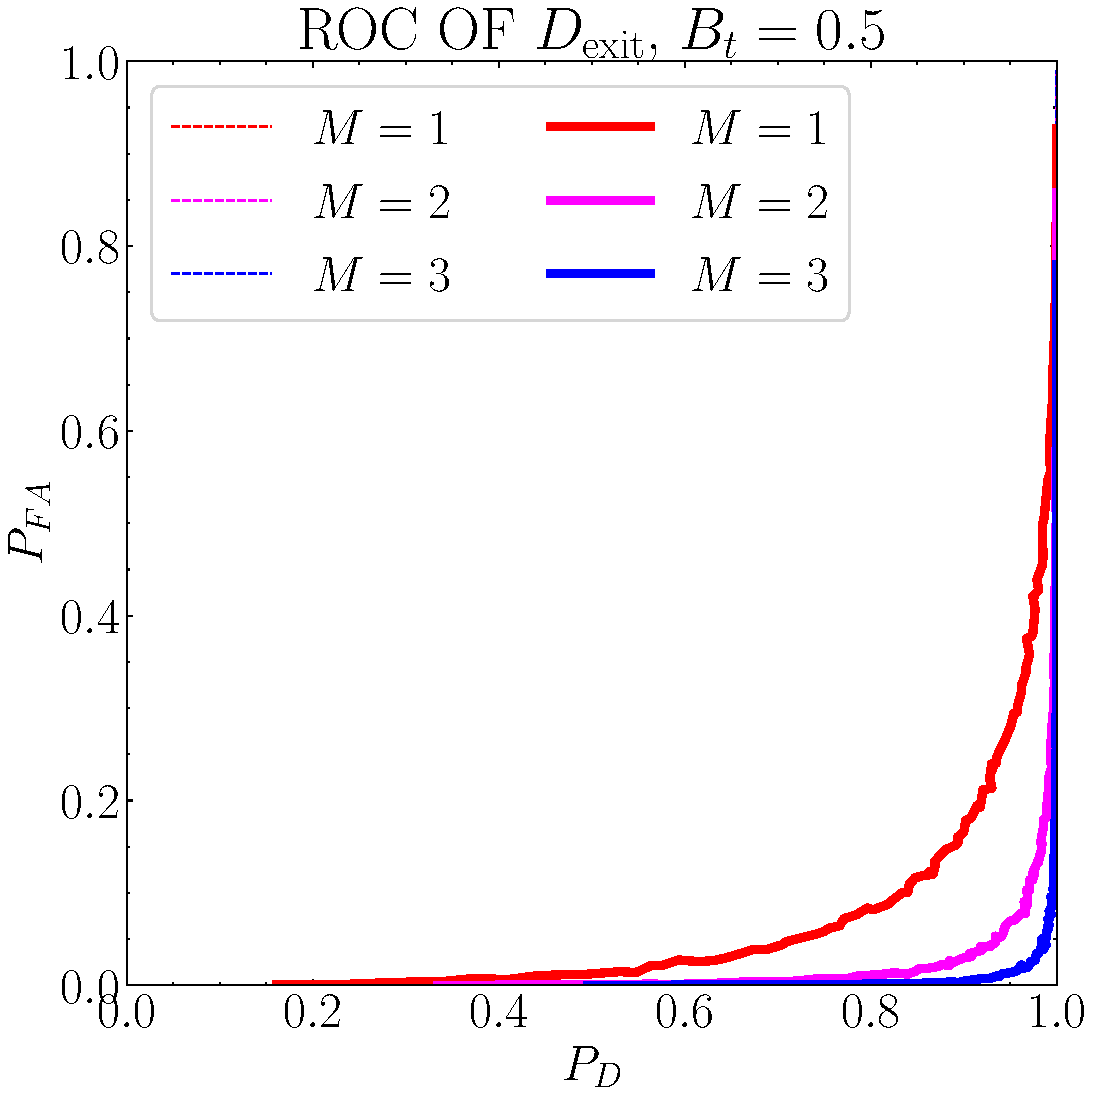
\includegraphics[width=2in]{../results/CFAR/CFAR_ROC_Bt_0.5}}
\subfigure[$B_{t}=0.6$]{\label{fig:a}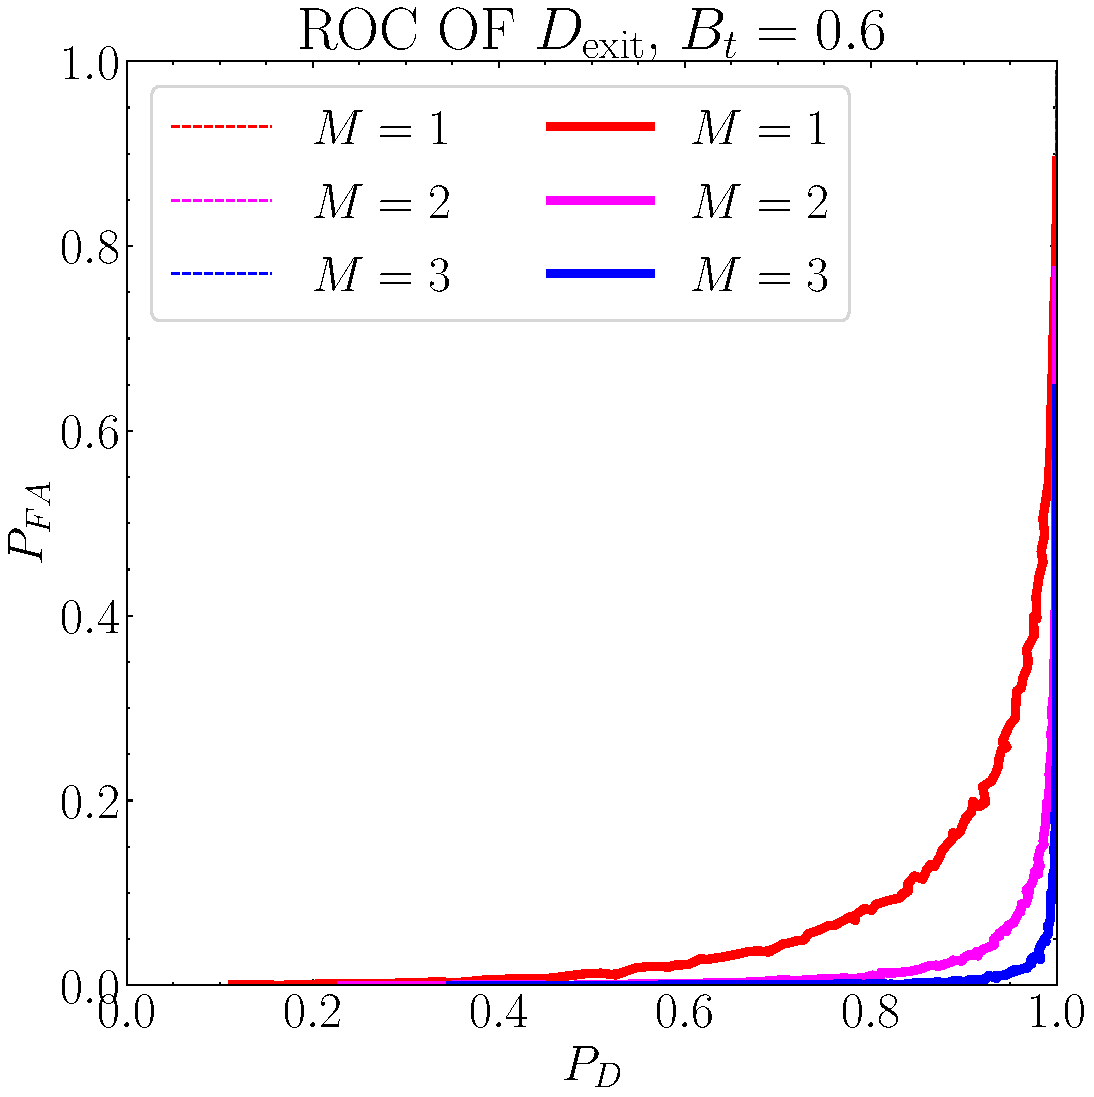
\includegraphics[width=2in]{../results/CFAR/CFAR_ROC_Bt_0.6}}
\caption{[Colour online] ROC for the detector for varying number of channels $M$, for each value of parameter $B_{t}$. Solid lines show the estimated ROC and dashed lines show the theoretical ROC.}
\label{fig:ROCdexit}
\end{figure}

Figure \ref{fig:ROCdexit} shows the ROC for $D_{\text{exit}}$ with varying number of channels $M$, and for each value of $B_{t}$. We observe that the ROC is identical for each setting $M$, over varying $B_{t}$. This shows that the detector is independent of $B_{t}$, as designed. For any given value of $B_{t}$, we observe the ROC is convex (axes are flipped, as compared to Figure \ref{fig:ROCdentry}), i.e., achieves high probability of detection for low probability of false alarm, and matches the theoretical ROC, in all cases with varying $M$. Between the ROC for varying $M$, we see that the ROC with a larger value for $M$ is more convex. This is, again, as expected as more channels implies more measurements.

% -----------------------------------------------------------------------------------------------------------------------
% -----------------------------------------------------------------------------------------------------------------------
 
\section{Part B: Vehicle Tracking}
\label{sec:partA_Tracking}

% -----------------------------------------------------------------------------------------------------------------------
% -----------------------------------------------------------------------------------------------------------------------

\subsection{Derivation}
\label{subsec:partB_derivation}

The deployed RADAR provides measurements of the position and velocity of the vehicle in 2 dimensions. We assume the vehicle moves with constant speed at the instants where the position and velocity are measured. Since the track has paths that mostly only have horizontal-only or vertical-only motions, constant speed implies constant velocity at each segment after which either the sign or the coordinate or both changes. The position and velocity maybe assumed to be unknown and maybe incorporated into the state model.

% -----------------------------------------------------------------------------------------------------------------------

\subsubsection{State model for Kalman filter}
\label{subsubsec:stateModel}

The vehicle dynamics, under constant speed, is fully described by its position vector $[p_{x}[n] \; p_{y}[n]]^{\TT}$ and velocity vector $[\dot{p}_{x}[n] \; \dot{p}_{y}[n]]^{\TT}$, at every time step $n=0,1,\cdots,N-1$. Hence, let the state variable be $\bx[n] = [p_{x}[n] \; p_{y}[n] \; \dot{p}_{x}[n] \; \dot{p}_{y}[n]]^{\TT}$. The equations of kinematics with constant motion, in general, are:
\begin{equation}
\begin{split}
	p_{x}[n] &= p_{x}[n-1] + \dot{p}_{x}[n-1] \Delta + w_{1}[n], \\
	p_{y}[n] &= p_{y}[n-1] + \dot{p}_{y}[n-1] \Delta + w_{2}[n], \\
	\dot{p}_{x}[n] &= \dot{p}_{x}[n-1] + w_{3}[n], \\
	\dot{p}_{y}[n] &= \dot{p}_{y}[n-1] + w_{4}[n], \\
	\text{i.e. }
	\bx[n] &= \underbrace{\begin{bmatrix}
		1 & 0 & \Delta & 0 \\
		0 & 1 & 0 & \Delta \\
		0 & 0 & 1 & 0 \\
		0 & 0 & 0 & 1
	\end{bmatrix}}_{\bA[n-1]} \bx[n-1] + \bw[n],
\end{split}
\label{eq:kinematicsGeneral}
\end{equation}
where $\bA[n]$ is the state-transition matrix and $\bw[n]$ is the noise vector at time step $n$ that accounts for model mismatch. We assume the noise vector is white Gaussian distributed with covariance matrix $\bQ_{w}[n]$. However, the state-transition matrix changes with the time step as the vehicle turns at the corners. Therefore, (\ref{eq:kinematicsGeneral}) is not valid for all (or maybe simplified at some) time steps.

Let $n_{X}$ denote the time step when the vehicle reaches the node $X$, where $X\in$ A,B,...,H. From A-B, B-C, D-E, E-F, F-G, H-A, i.e., $n=0,1,\cdots,n_{B}, n_{B}+1,n_{B}+2,\cdots,n_{C}-1, n_{D}+1,n_{D}+2,\cdots,n_{E}-1, n_{E}+1,n_{E}+2,\cdots,n_{F}-1, n_{F}+1,n_{F}+2,\cdots,n_{G}-1, n_{H}+1,n_{H}+2,\cdots,N-1$, we can set $\dot{p}_{x}[n] = 0$. At B, E, F, i.e., $n=n_{B}, n_{E}, n_{F}$, $\dot{p}_{y}[n] = -\dot{p}_{y}[n-1] + w_{4}[n]$. At C, G, i.e., $n=n_{C},n_{G}$, we have $\dot{p}_{x}[n] = -\dot{p}_{y}[n-1]$ and $\dot{p}_{y}[n] = 0$. From C-D, G-H, i.e., $n=n_{C}+1,n_{C}+2,\cdots,n_{D}-1, n_{G}+1,n_{G}+2,\cdots,n_{H}-1$, we can set $\dot{p}_{y}[n] = 0$ in (\ref{eq:kinematicsGeneral}). At D, H, i.e., $n=n_{D}, n_{H}$, we have $\dot{p}_{y}[n] = -\dot{p}_{x}[n-1]$ and $\dot{p}_{x}[n]=0$. This gives the following as the state matrix:
\begin{equation}
	\bA[n] = \begin{cases}
		\begin{bmatrix}
			1 & 0 & 0 & 0 \\
			0 & 1 & 0 & \Delta \\
			0 & 0 & 0 & 0 \\
			0 & 0 & 0 & 1
		\end{bmatrix} & ;n<n_{C}, n_{D}<n<n_{F}, n_{H}<n, \\
		\begin{bmatrix}
			1 & 0 & 0 & 0 \\
			0 & 1 & 0 & \Delta \\
			0 & 0 & 0 & -1 \\
			0 & 0 & 0 & 0
		\end{bmatrix} & ;n=n_{C},n_{G}, \\
		\begin{bmatrix}
			1 & 0 & \Delta & 0 \\
			0 & 1 & 0 & 0 \\
			0 & 0 & 0 & 0 \\
			0 & 0 & -1 & 0
		\end{bmatrix} & ;n=n_{D},n_{H}, \\
		\begin{bmatrix}
			1 & 0 & \Delta & 0 \\
			0 & 1 & 0 & 0 \\
			0 & 0 & 1 & 0 \\
			0 & 0 & 0 & 0
		\end{bmatrix} & ;\text{otherwise}. \\
	\end{cases}
\end{equation}

% -----------------------------------------------------------------------------------------------------------------------

\subsubsection{Kalman filter using velocity measurements}
\label{subsubsec:velocityKalmanFilter}

Consider the vehicle with the state equation $\bx[n] = \bA[n-1]\bx[n-1] + \bw[n]$, with the state variable measured using:
\begin{equation}
	\by[n] = \underbrace{\begin{bmatrix}
		0 & 0 & 1 & 0 \\
		0 & 0 & 0 & 1
	\end{bmatrix}}_{\bC[n]} \bx[n-1] + \bv[n], \; n=0,1,\cdots,N-1,
\label{eq:velMeasurements}
\end{equation}
where $\bv[n]$ is the measurement noise. We assume the measurement noise is i.i.d zero mean Gaussian distributed with covariance matrix $\bQ_{v}[n]$. The Kalman filter updates for the state variable and the error covariance are then given by:
\begin{equation}
\begin{split}
	\hat{\bx}[n|n-1] &= \bA[n-1] \hat{\bx}[n-1|n-1], \\
	\bP[n|n-1] &= \bA[n-1] \bP[n-1|n-1] \bA^{\TT}[n-1] + \bQ_{w}[n],
\end{split}
\label{eq:kalmanUpdate}
\end{equation}
and the Kalman filter predictions are given by:
\begin{equation}
\begin{split}
	\hat{\bx}[n|n] &= \hat{\bx}[n|n-1] + \bK[n] \left( y[n] - \bC[n]\hat{\bx}[n|n-1] \right), \\
	\bP[n|n] &= \left(\bI - \bK[n]\bC[n]\right)\bP[n|n-1],
\end{split}
\label{eq:kalmanPredict}
\end{equation}
where the Kalman gain is given by $\bK[n] = \bP[n|n-1]\bC^{\TT}[n]\left(\bQ_{v}+\bC[n]\bP[n|n-1]\bC^{\TT}[n]\right)^{-1}$.

% -----------------------------------------------------------------------------------------------------------------------

\subsubsection{Kalman filter using position and velocity measurements}
\label{subsubsec:fullKalmanFilter}

Consider the vehicle with the state equation $\bx[n] = \bA[n-1]\bx[n-1] + \bw[n]$, with the state variable measured using:
\begin{equation}
	\by[n] =  \bx[n-1] + \bv[n], \; n=0,1,\cdots,N-1,
\label{eq:stateMeasurements}
\end{equation}
where $\bv[n]$ is the measurement noise. We assume the measurement noise is i.i.d zero mean Gaussian distributed with covariance matrix $\bQ_{v}[n]$. The Kalman filter updates are identical to (\ref{eq:kalmanUpdate}) and predictions are identical to (\ref{eq:kalmanPredict}) with $\bC[n] = \bI$. The Kalman filter predictions:
\begin{equation}
\begin{split}
	\hat{\bx}[n|n] &= \hat{\bx}[n|n-1] + \bK[n] \left( y[n] - \hat{\bx}[n|n-1] \right), \\
	\bP[n|n] &= \left(\bI - \bK[n]\right)\bP[n|n-1],
\end{split}
\label{eq:kalmanPosPredict}
\end{equation}
where the Kalman gain is given by $\bK[n] = \bP[n|n-1]\left(\bQ_{v}+\bP[n|n-1]\right)^{-1}$.

% -----------------------------------------------------------------------------------------------------------------------
% -----------------------------------------------------------------------------------------------------------------------

\subsection{Implementation}
\label{subsec:partB_implementation}

% -----------------------------------------------------------------------------------------------------------------------

\subsubsection{Kalman filter with velocity only measurements}
\label{subsubsec:kalmanVelocity}

We implement Kalman filter with velocity-only measurements using the state model as in (\ref{eq:kinematicsGeneral}) and measurement model as in (\ref{eq:velMeasurements}). We consider RADAR measurements of velocity with measurement noise $\bQ_{v}=0.1\bI$. We set the model noise $\bQ_{w}=0.1\bI$ and consider two initialisations: first with the correct initial position $\hat{x}[0|0] = \zerovec$, and second with an offset to the position with $\hat{x}[0|0] = [1\;0\;0\;0]^{\TT}$. We determine the tracking performance using the squared-error between the Kalman filter predictions of position ($\hat{\mathbf{p}}[n]$) and the true trace ($\mathbf{p}[n]$), and compare it to the squared error between the RADAR measurements and the true trace.
\begin{figure}[h!]
\centering
%\subfigure[Trace $\bQ_{w}=\zerovec, \hat{\bx}(0|0)=\zerovec$]{\label{fig:a}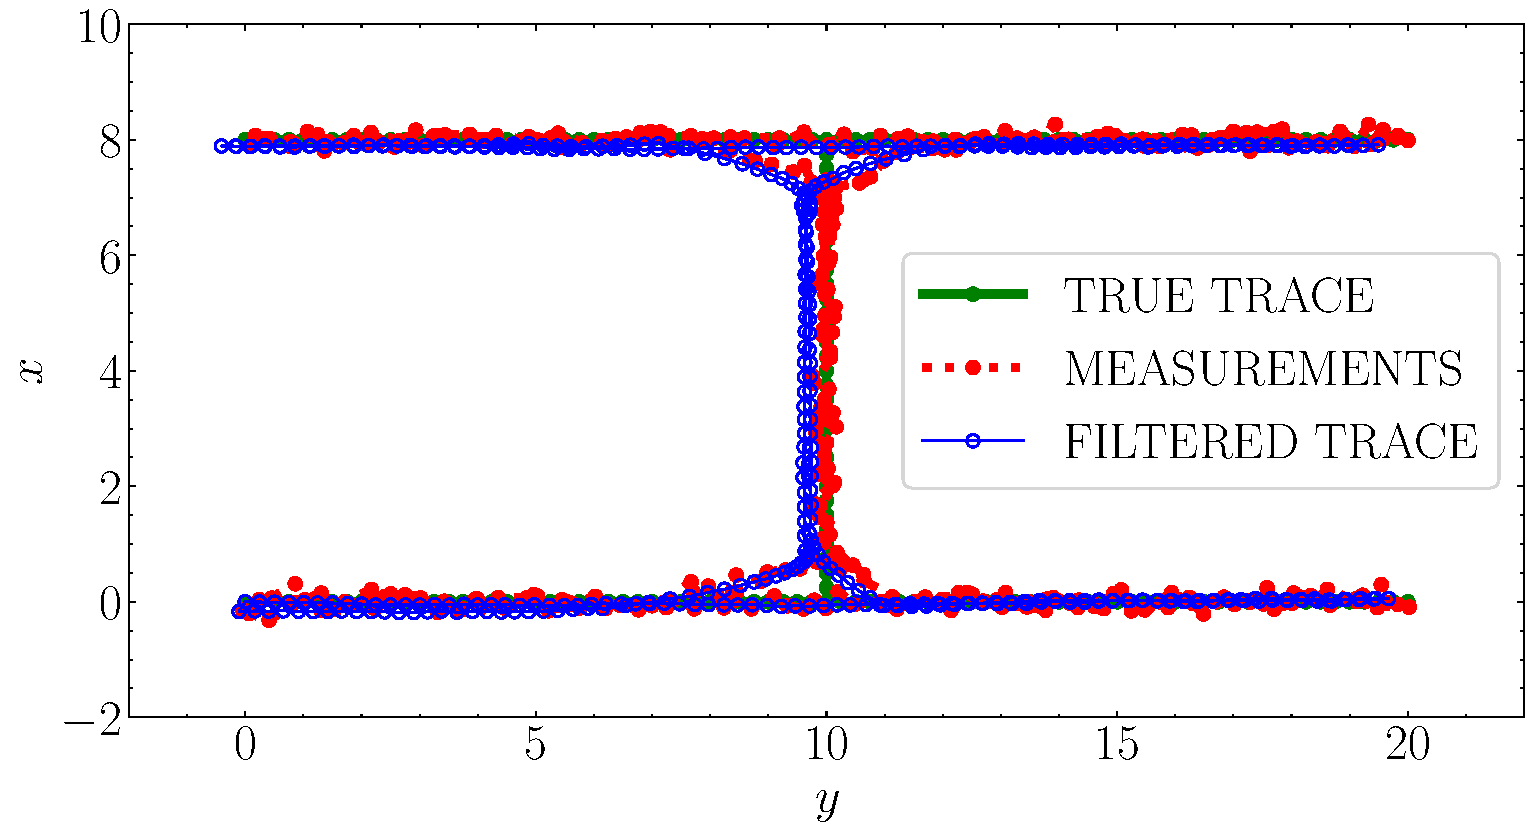
\includegraphics[width=3in]{../results/KF/ex1/KF_Vel_Trace_Init_exact_noise_0.0}}
%\subfigure[Error, $\bQ_{w}=\zerovec, \hat{\bx}(0|0)=\zerovec$]{\label{fig:a}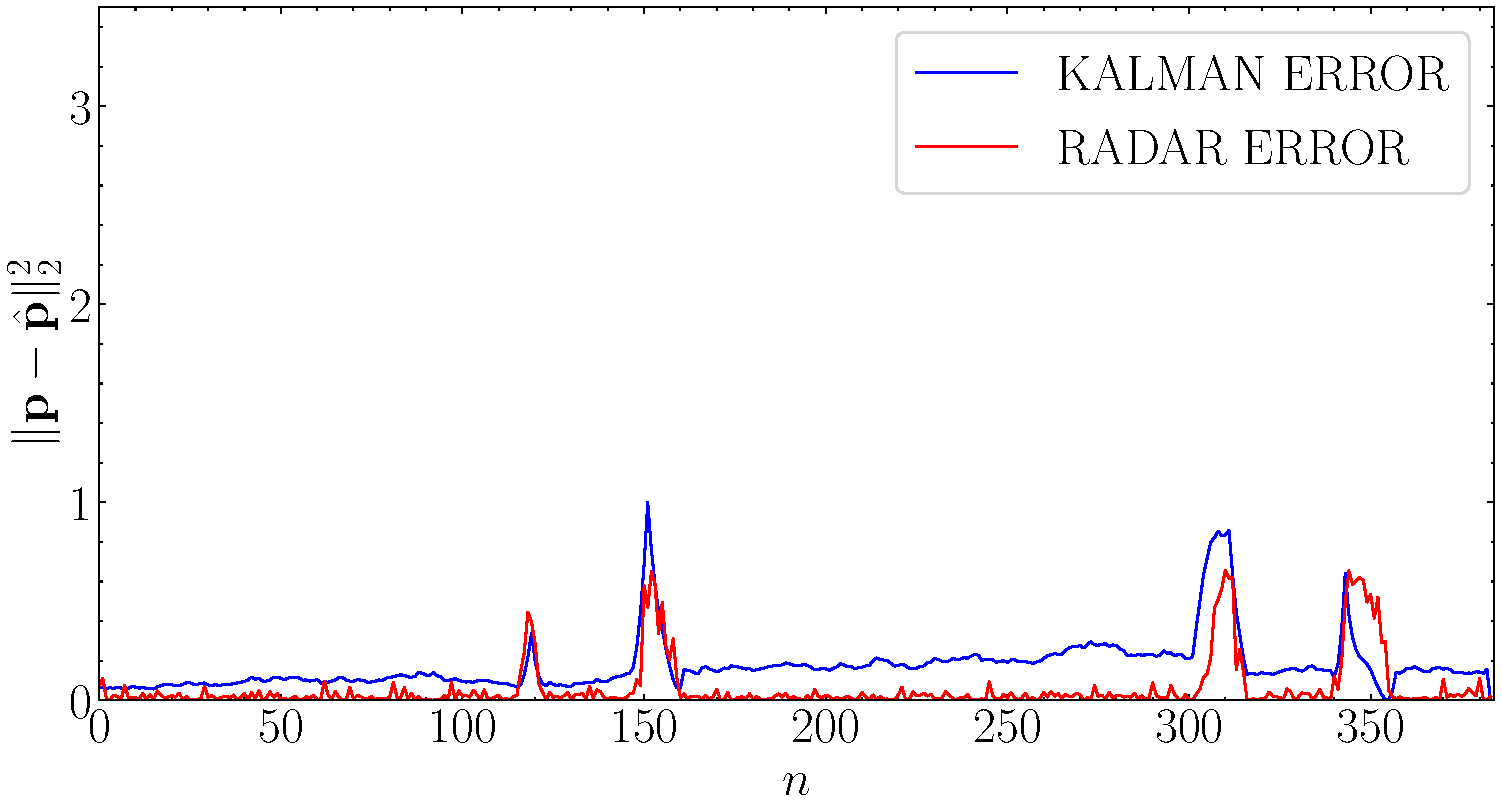
\includegraphics[width=3in]{../results/KF/ex1/KF_Vel_Errors_Init_exact_noise_0.0}}
%
%\subfigure[Trace $\bQ_{w}=\zerovec, \hat{\bx}(0|0)\neq\zerovec$]{\label{fig:a}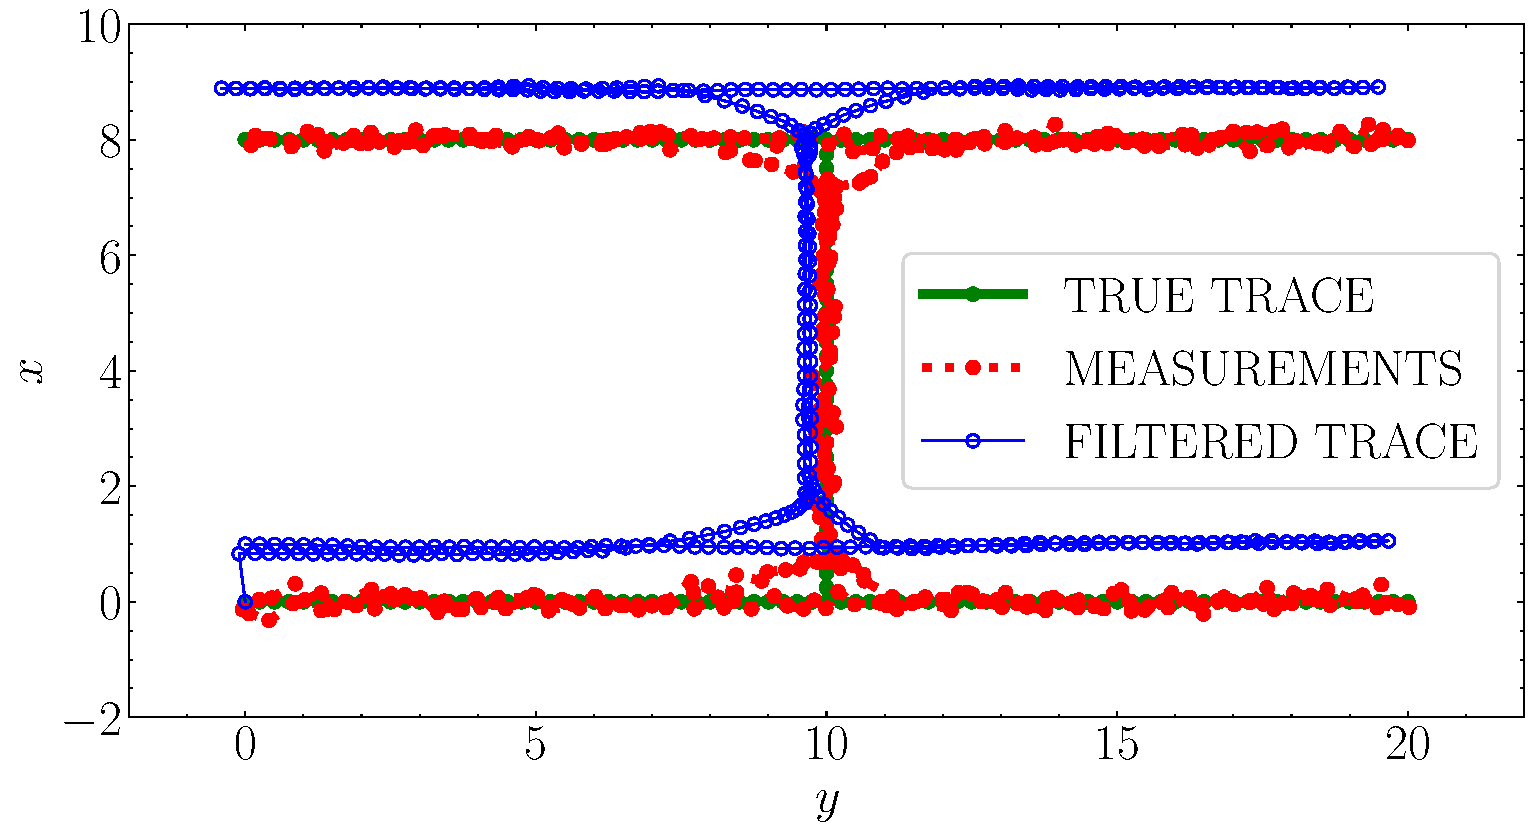
\includegraphics[width=3in]{../results/KF/ex1/KF_Vel_Trace_Init_bias_noise_0.0}}
%\subfigure[Error, $\bQ_{w}=\zerovec, \hat{\bx}(0|0)\neq\zerovec$]{\label{fig:a}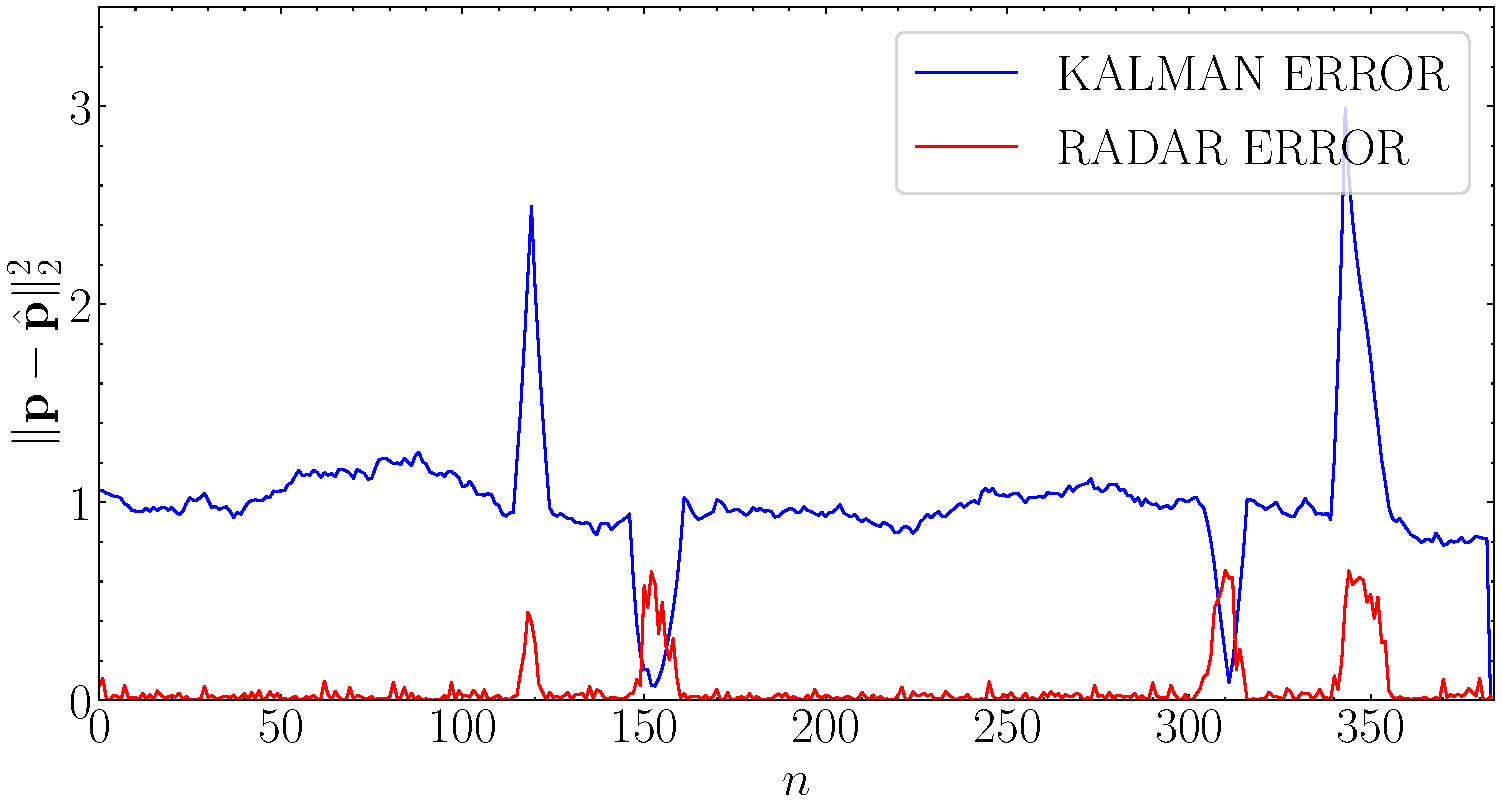
\includegraphics[width=3in]{../results/KF/ex1/KF_Vel_Errors_Init_bias_noise_0.0}}
\subfigure[Trace $\bQ_{w}=0.1\bI, \hat{\bx}(0|0)=\zerovec$]{\label{fig:a}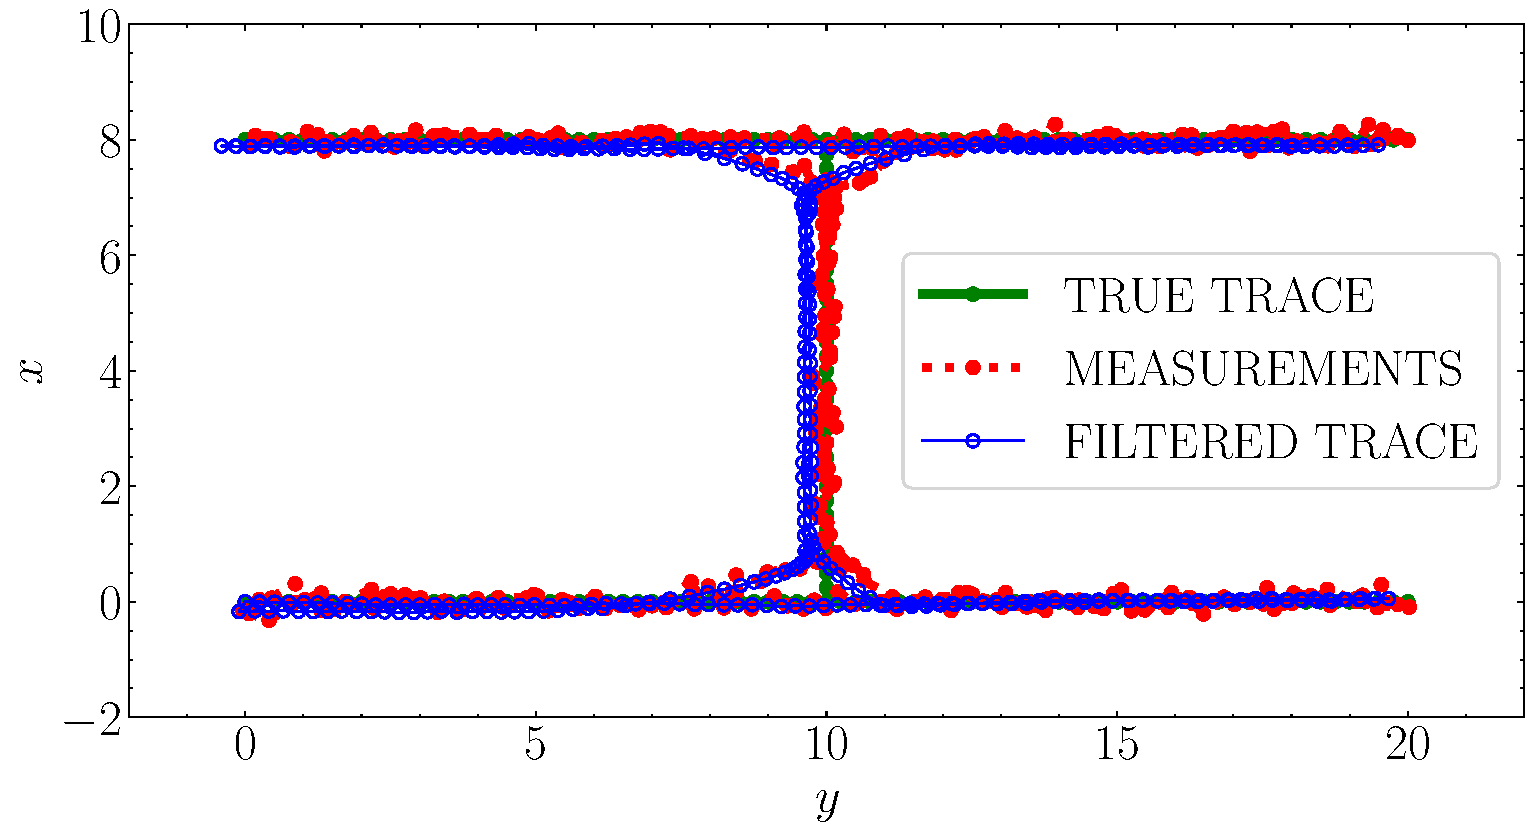
\includegraphics[width=3in]{../results/KF/ex1/KF_Vel_Trace_Init_exact_noise_0.1}}
\subfigure[Error, $\bQ_{w}=0.1\bI, \hat{\bx}(0|0)=\zerovec$]{\label{fig:a}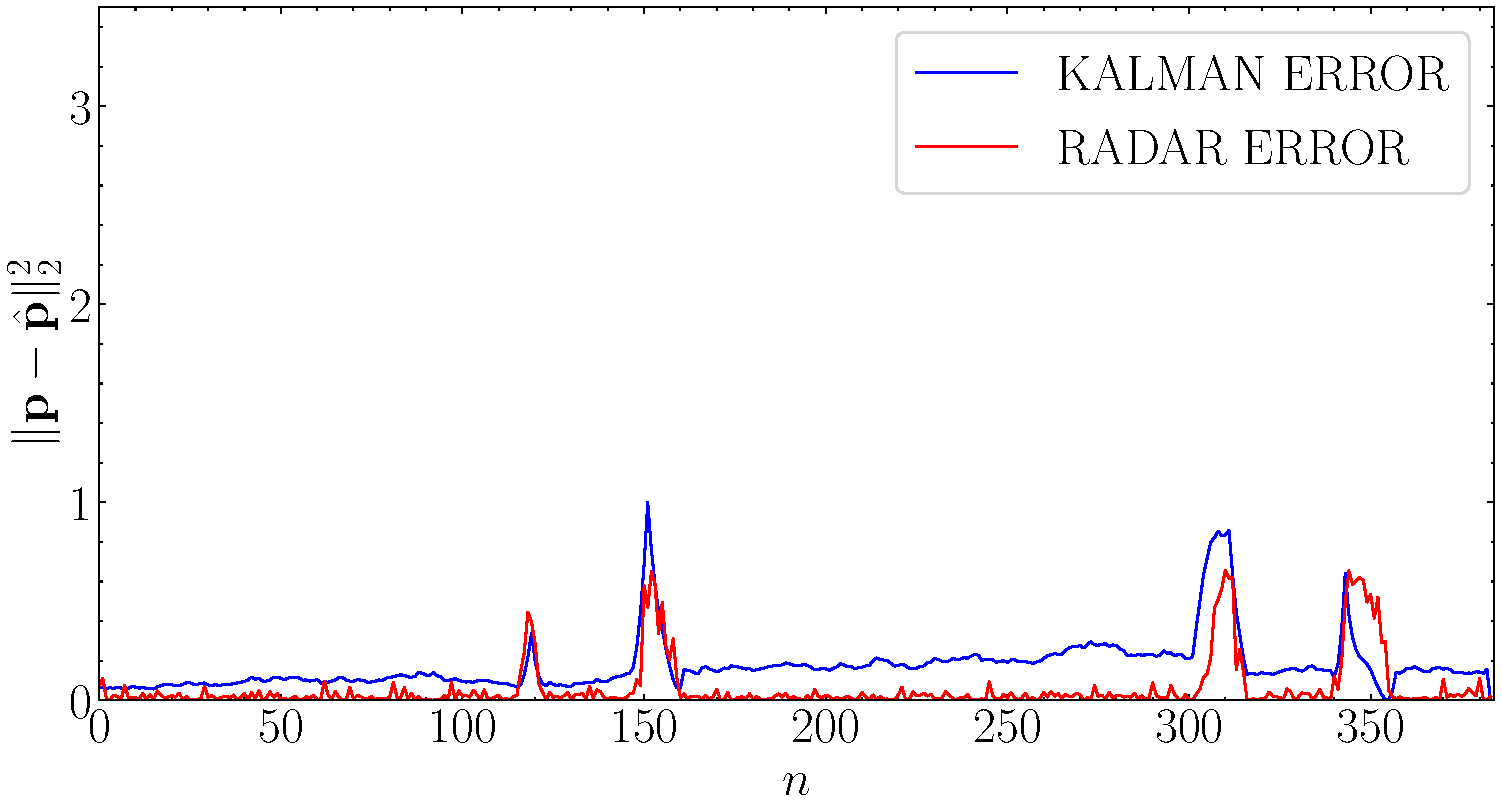
\includegraphics[width=3in]{../results/KF/ex1/KF_Vel_Errors_Init_exact_noise_0.1}}

\subfigure[Trace $\bQ_{w}=0.1\bI, \hat{\bx}(0|0)\neq\zerovec$]{\label{fig:a}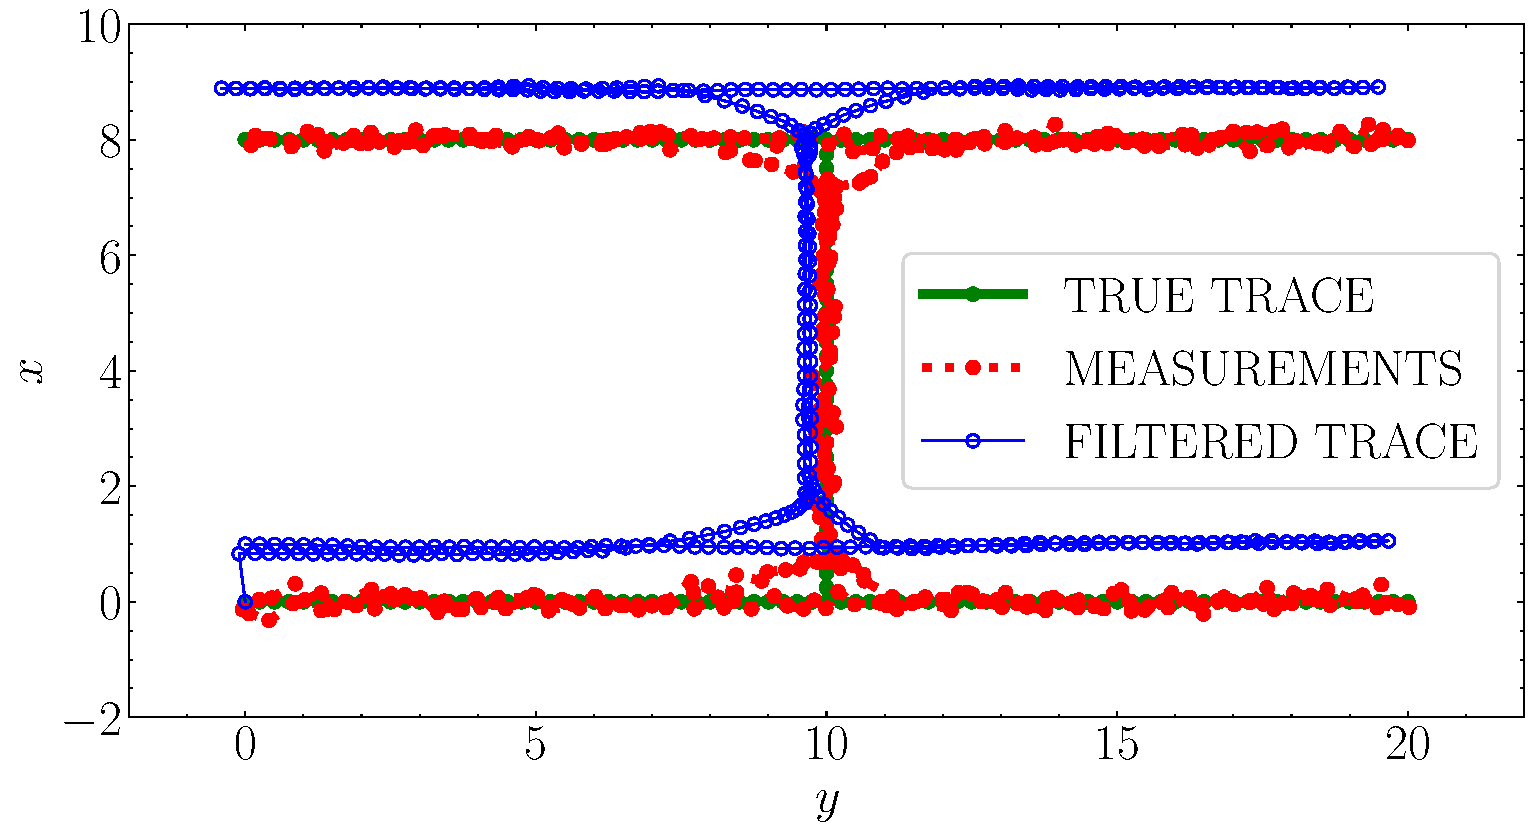
\includegraphics[width=3in]{../results/KF/ex1/KF_Vel_Trace_Init_bias_noise_0.1}}
\subfigure[Error, $\bQ_{w}=0.1\bI, \hat{\bx}(0|0)\neq\zerovec$]{\label{fig:a}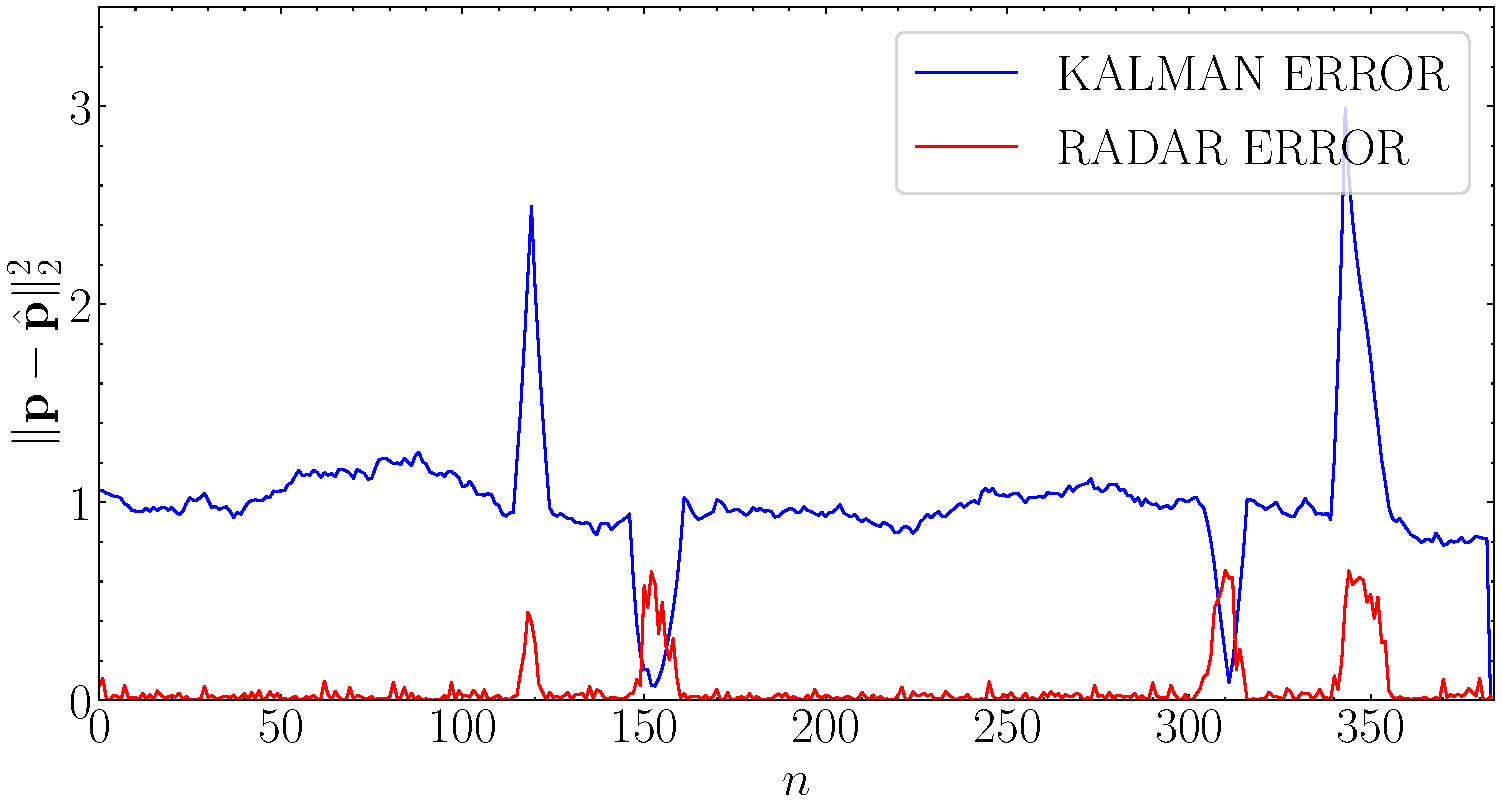
\includegraphics[width=3in]{../results/KF/ex1/KF_Vel_Errors_Init_bias_noise_0.1}}
\caption{[Colour online] Figures show the Kalman filter prediction and RADAR measurements compared to the true trace. The first column shows the traces and the second column shows the errors, for different initialisations and model noise.}
\label{fig:TraceVel}
\end{figure}

Figure \ref{fig:TraceVel} shows the trace and the errors for the two cases of initialisation. We observe that the tracking in case of initialisation with $\hat{x}[0|0] = \zerovec$ is fairly good. The error of the Kalman filter predictions matches the error in the RADAR measurements with an offset. The offset is much larger in the second case when the initialisation is set to $\hat{x}[0|0] = [1\;0\;0\;0]^{\TT}$. The trace shows that the tracking is off by the same amount the initialisation is off, throughout the trace. This is a feature of any position tracking algorithm from velocity measurements.

Estimation of position from velocity measurements needs solving first order system. The solutions are accurate up to a constant, if initial values are not available or are incorrect. In the first case, when the initial values are correct, the tracking is fairly decent. However, the second case, the tracking is poor, but the solution, as expected, is offset by the initialisation. Further, note that the Kalman filter predictions find the turns the vehicle takes, even though such motions are not allowed according to the state model. This is because the model noise $\bQ_{w}=0.1\bI$ allows some model mismatch. However, since only velocity measurements are available, the tracking at turns also has additional bias.

Suppose the measurements are clean ($\bQ_{v}=\zerovec$) and the vehicle always moves with a constant speed ($\bQ_{w}=\zerovec$), it is possible to accurately track the position of the vehicle only up to a constant offset. This offset maybe removed by correctly initialising the Kalman filter.

% -----------------------------------------------------------------------------------------------------------------------

\subsubsection{Kalman filter with position and velocity measurements}
\label{subsubsec:kalmanPostionVelocity}

We implement the Kalman filter using both position and velocity measurements using the state model in (\ref{eq:kinematicsGeneral}) and measurement model as in (\ref{eq:stateMeasurements}). We consider RADAR measurements of both position and velocity with measurement noise $\bQ_{v}=0.1\bI$. We vary the model noise $\bQ_{w}\in\{0.01\bI,0.1\bI,\bI\}$ and initialise the Kalman filter with $\hat{x}[0|0] = \zerovec$. We determine the tracking performance using the squared-error between the Kalman filter predictions of position ($\hat{\mathbf{p}}[n]$) and the true trace ($\mathbf{p}[n]$), and compare it to the squared error between the RADAR measurements and the true trace.
\begin{figure}[h!]
\centering
\subfigure[Trace $\bQ_{w}=0.01\bI$]{\label{fig:a}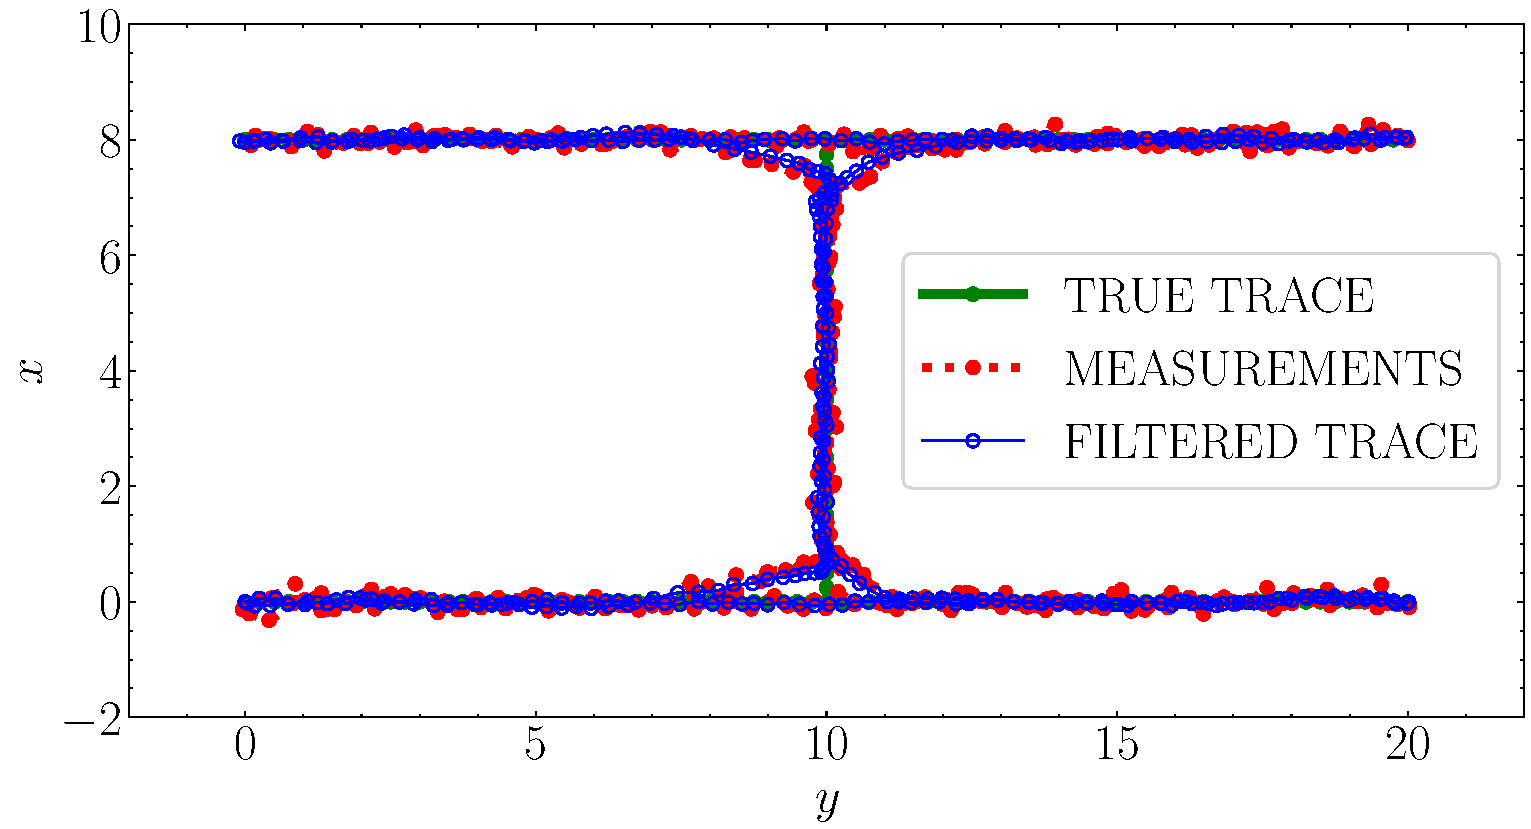
\includegraphics[width=3in]{../results/KF/ex2/KF_Pos_Trace_Data_med_noise_0.01}}
\subfigure[Error, $\bQ_{w}=0.01\bI$]{\label{fig:a}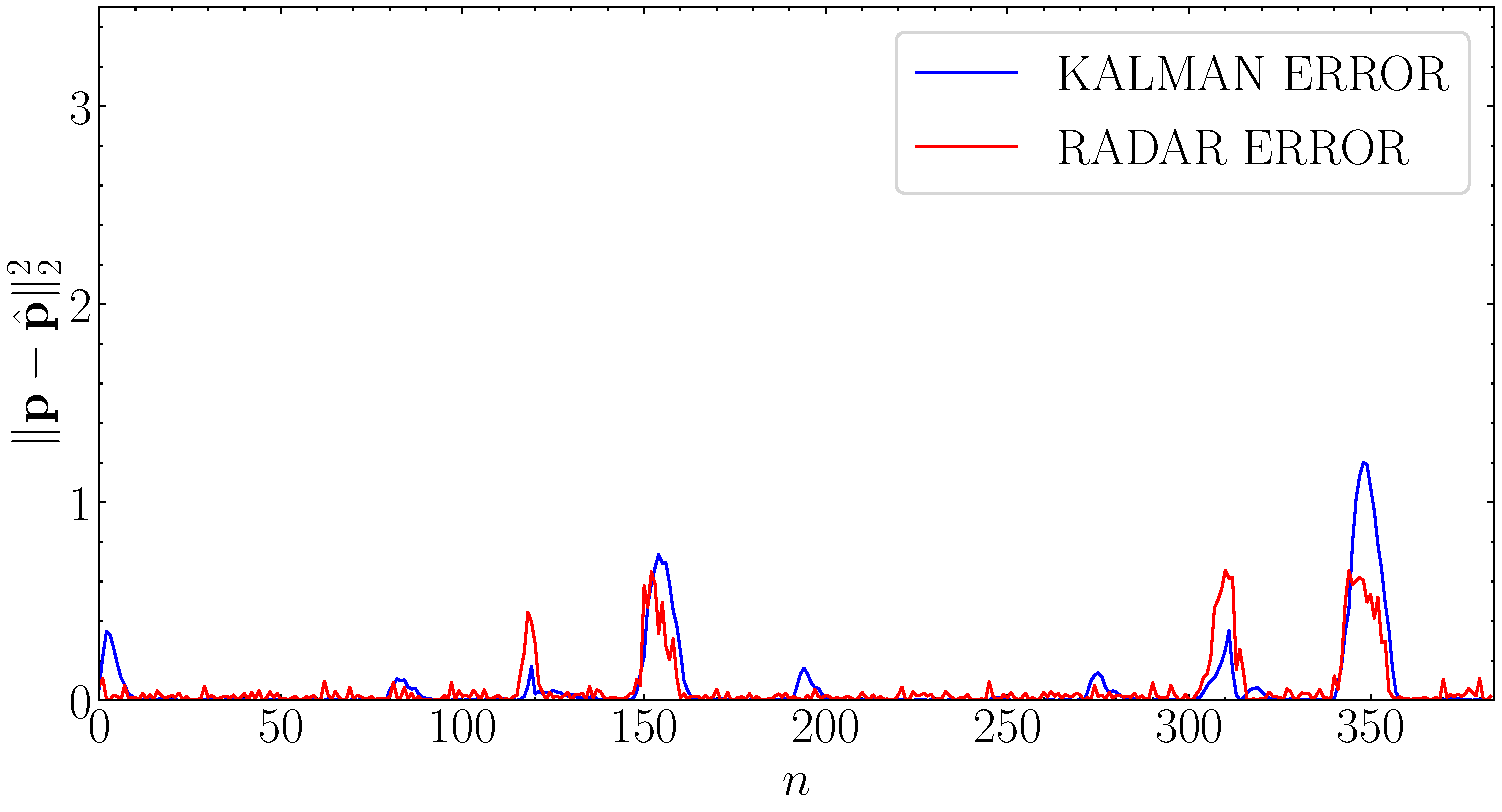
\includegraphics[width=3in]{../results/KF/ex2/KF_Pos_Errors_Data_med_noise_0.01}}

\subfigure[Trace $\bQ_{w}=0.1\bI$]{\label{fig:a}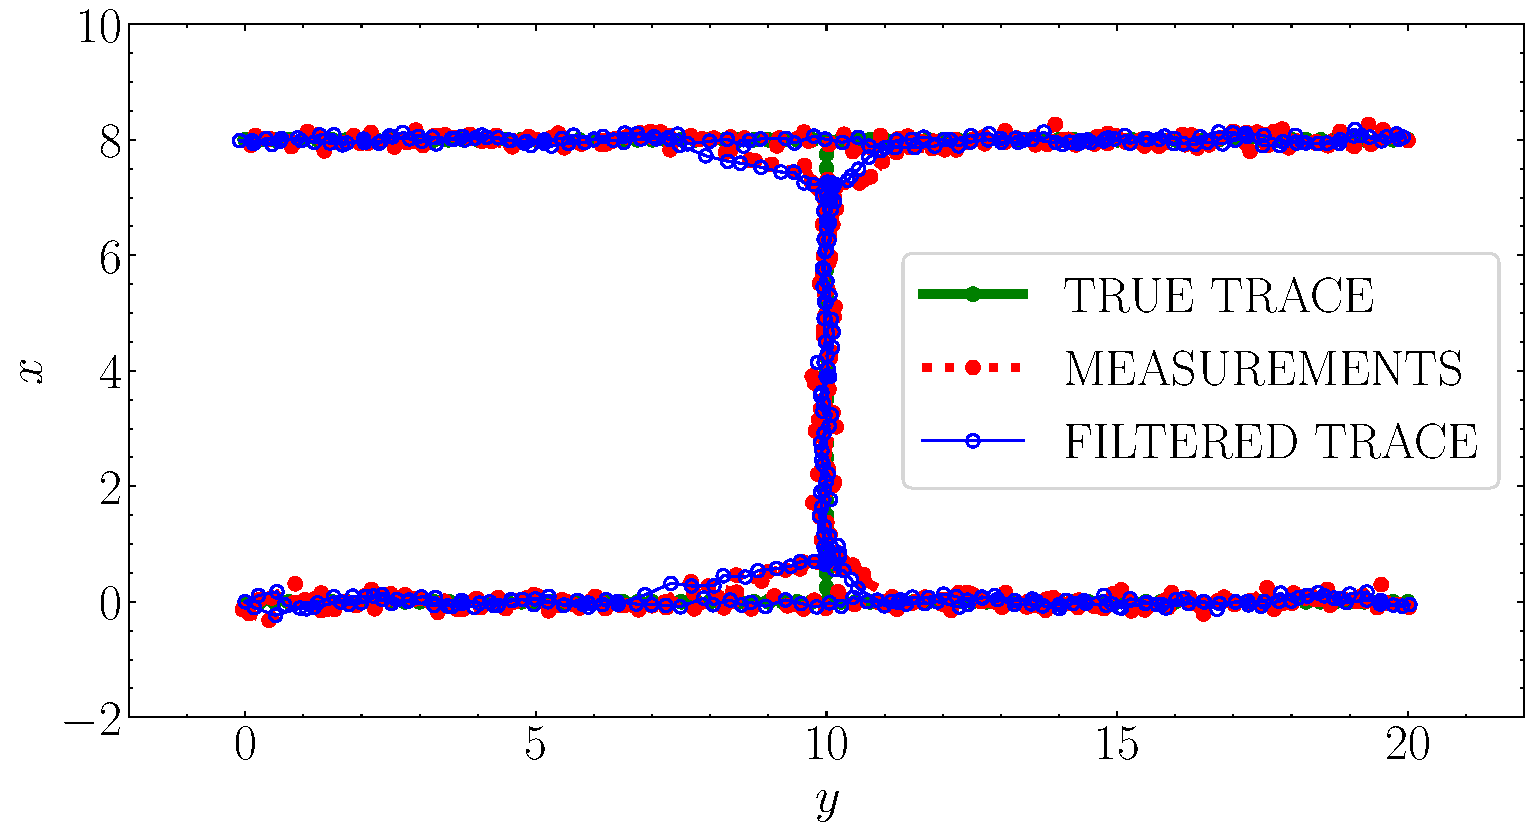
\includegraphics[width=3in]{../results/KF/ex2/KF_Pos_Trace_Data_med_noise_0.1}}
\subfigure[Error, $\bQ_{w}=0.1\bI$]{\label{fig:a}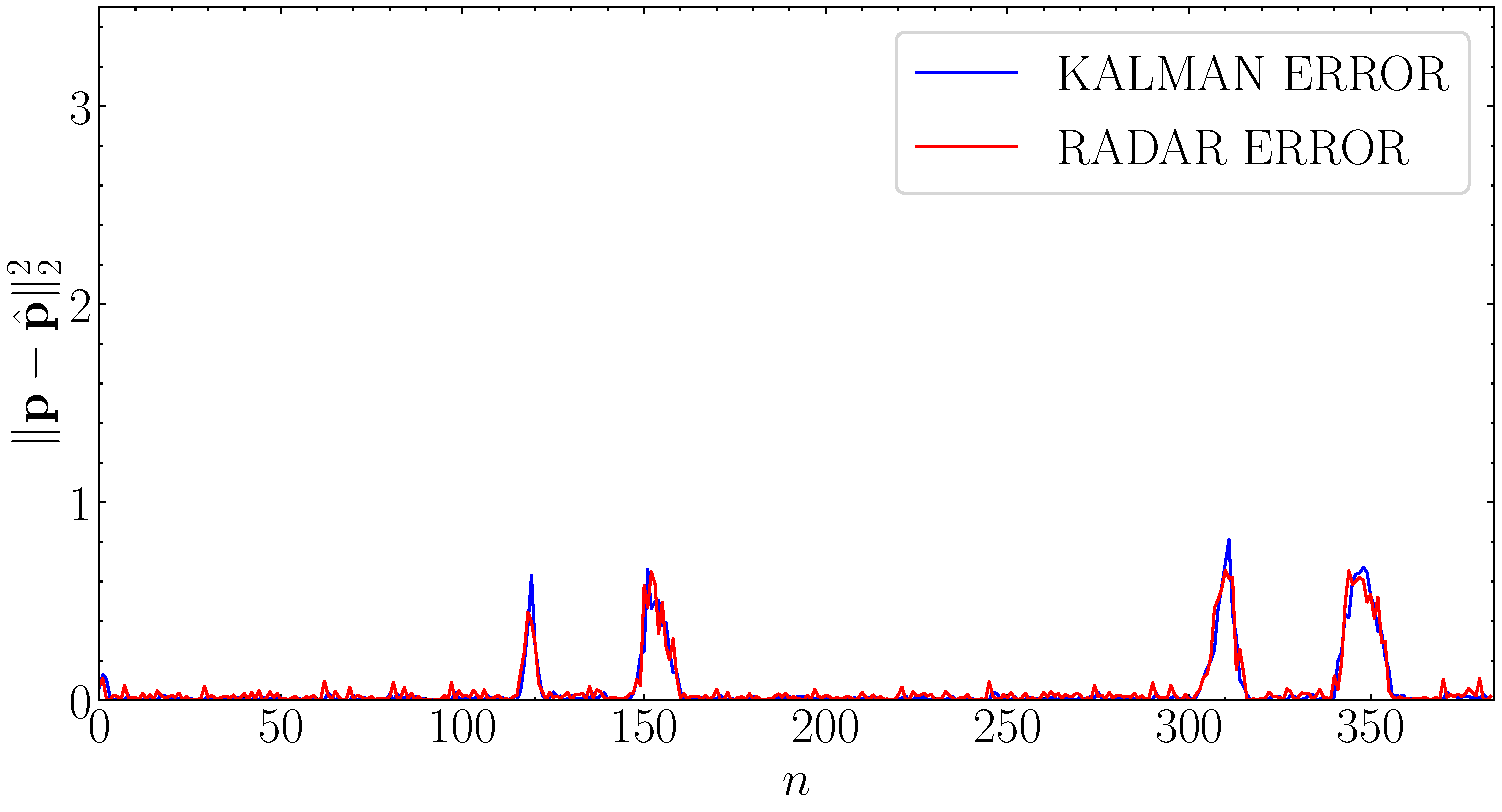
\includegraphics[width=3in]{../results/KF/ex2/KF_Pos_Errors_Data_med_noise_0.1}}

\subfigure[Trace $\bQ_{w}=\bI$]{\label{fig:a}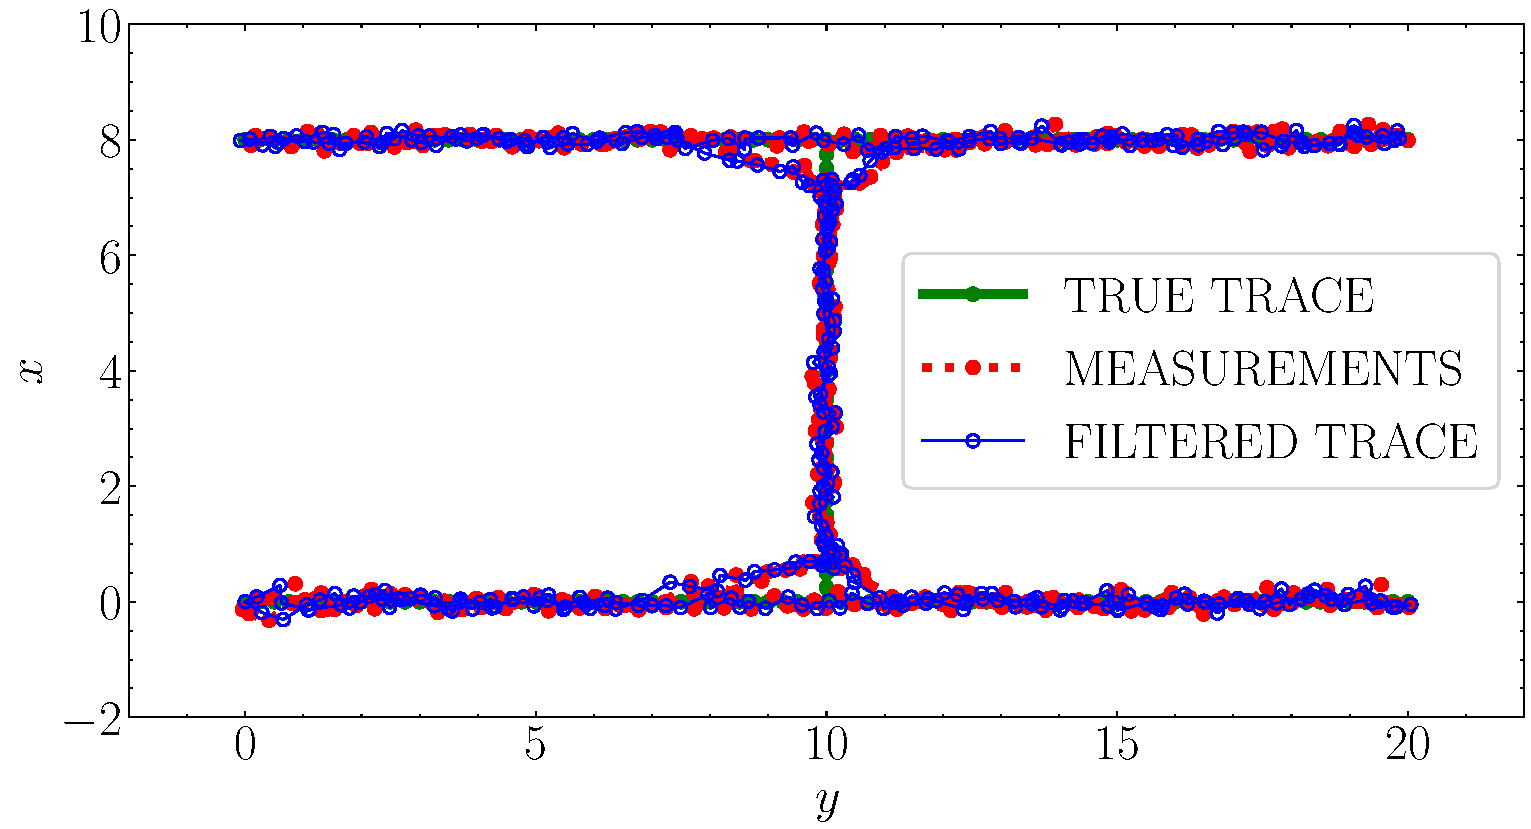
\includegraphics[width=3in]{../results/KF/ex2/KF_Pos_Trace_Data_med_noise_1.0}}
\subfigure[Error, $\bQ_{w}=\bI$]{\label{fig:a}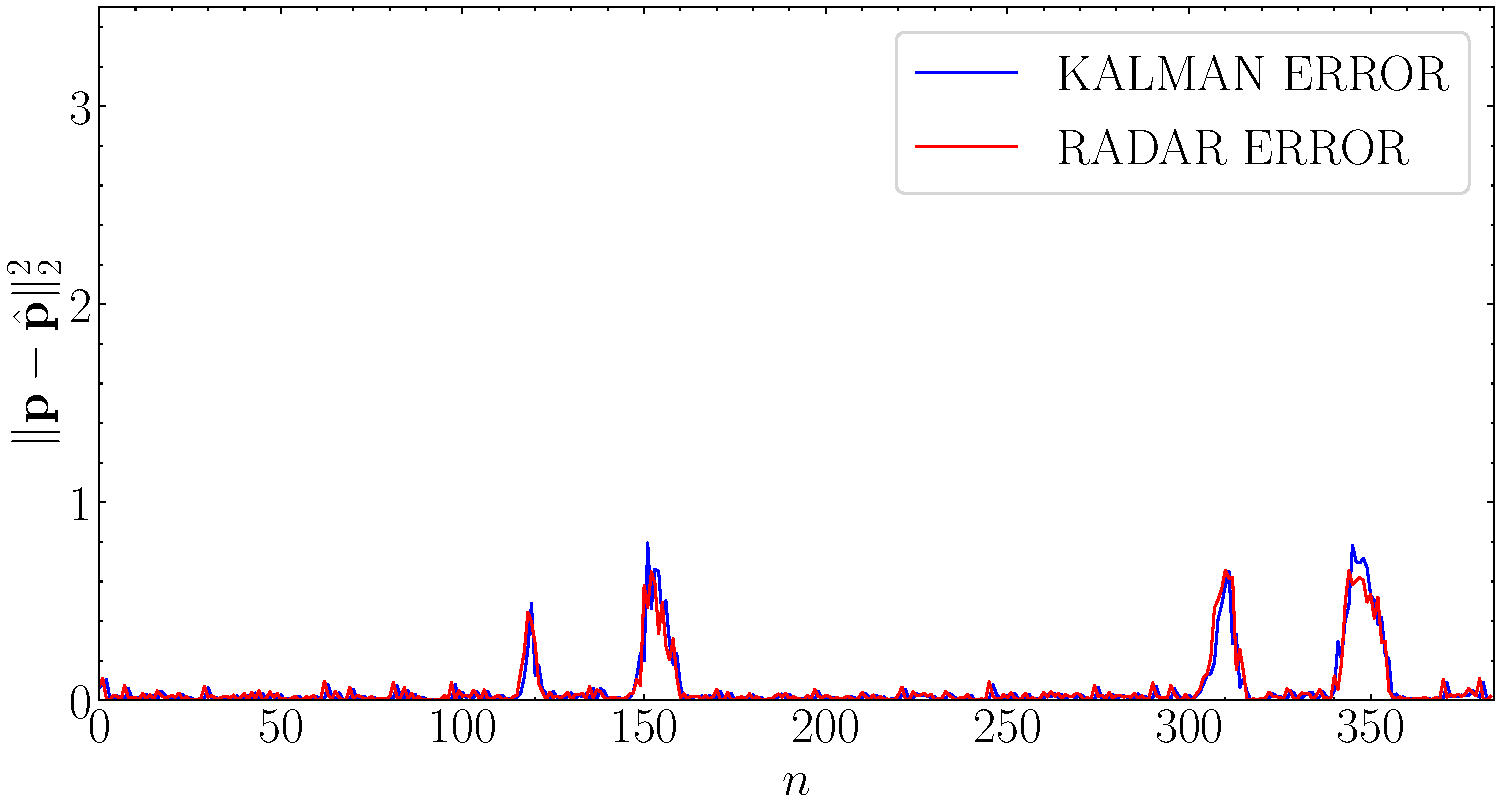
\includegraphics[width=3in]{../results/KF/ex2/KF_Pos_Errors_Data_med_noise_1.0}}
\caption{[Colour online] Figures show the Kalman filter prediction and RADAR measurements compared to the true trace. The first column shows the traces and the second column shows the errors, for different model noise, under measurements with $\bQ_{v}=0.1\bI$.}
\label{fig:TraceVelPosMed}
\end{figure}

Figure \ref{fig:TraceVelPosMed} shows the trace and errors for the three cases of model noise. We observe the Kalman filter predictions perform well in all three cases, at tracking when the model is accurately followed, i.e., at all points that do not include a turn. However, at turns, we see that the error with lower values of model noise is higher. This is because the measurements do not strictly follow the model in (\ref{eq:kinematicsGeneral}), where smooth turns are not allowed. When the model noise is low, the tracking error is high wherever the model mismatch is high. We see that the error at turns in the Kalman filter predictions matches the error in the RADAR measurements as the model noise increases.

% -----------------------------------------------------------------------------------------------------------------------

\subsubsection{Kalman filter with noisy measurements}
\label{subsubsec:kalmanNoisy}

We implement the Kalman filter using both position and velocity measurements using the state model in (\ref{eq:kinematicsGeneral}) and measurement model as in (\ref{eq:stateMeasurements}). We consider RADAR measurements of both position and velocity with measurement noise $\bQ_{v}=\bI$. We vary the model noise $\bQ_{w}\in\{0.0001\bI,0.01\bI,0.1\bI,\bI\}$ and initialise the Kalman filter with $\hat{x}[0|0] = \zerovec$. We determine the tracking performance using the squared-error between the Kalman filter predictions of position ($\hat{\mathbf{p}}[n]$) and the true trace ($\mathbf{p}[n]$), and compare it to the squared error between the RADAR measurements and the true trace.
\begin{figure}[h!]
\centering
\subfigure[Trace $\bQ_{w}=0.0001\bI$]{\label{fig:a}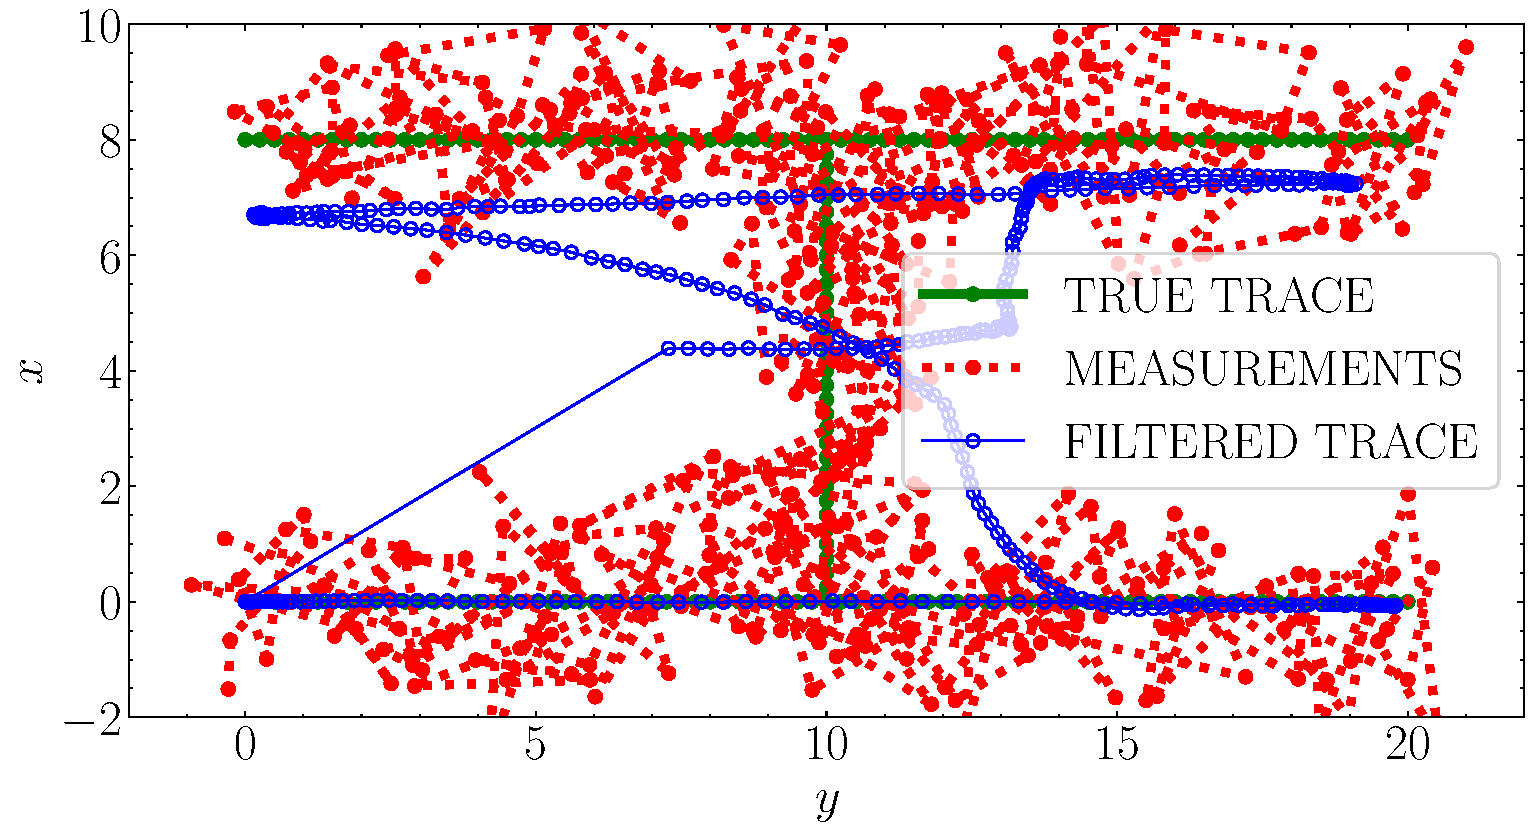
\includegraphics[width=3in]{../results/KF/ex3/KF_Pos_Trace_Data_high_noise_0.0001}}
\subfigure[Error, $\bQ_{w}=0.0001\bI$]{\label{fig:a}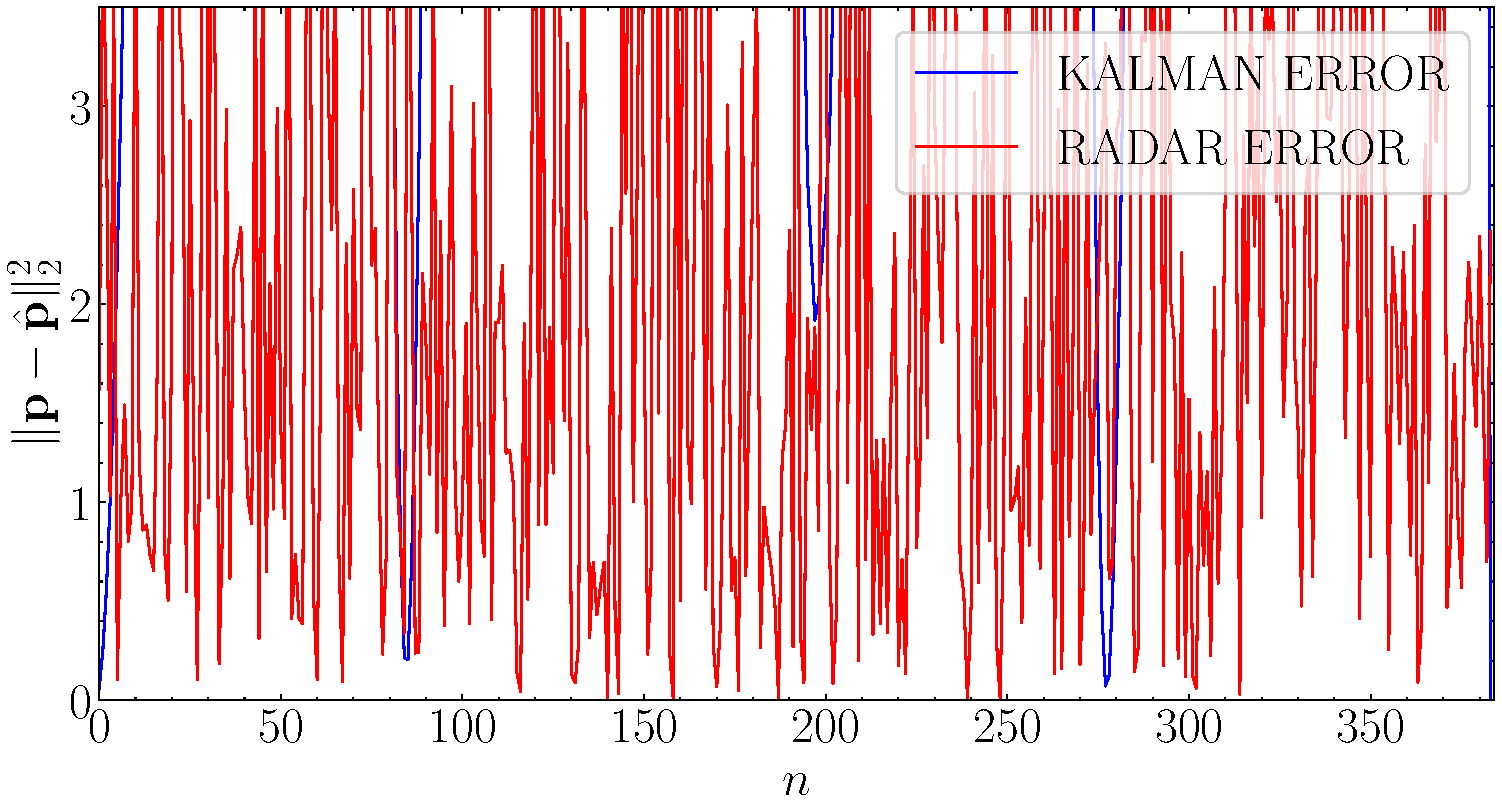
\includegraphics[width=3in]{../results/KF/ex3/KF_Pos_Errors_Data_high_noise_0.0001}}

\subfigure[Trace $\bQ_{w}=0.01\bI$]{\label{fig:a}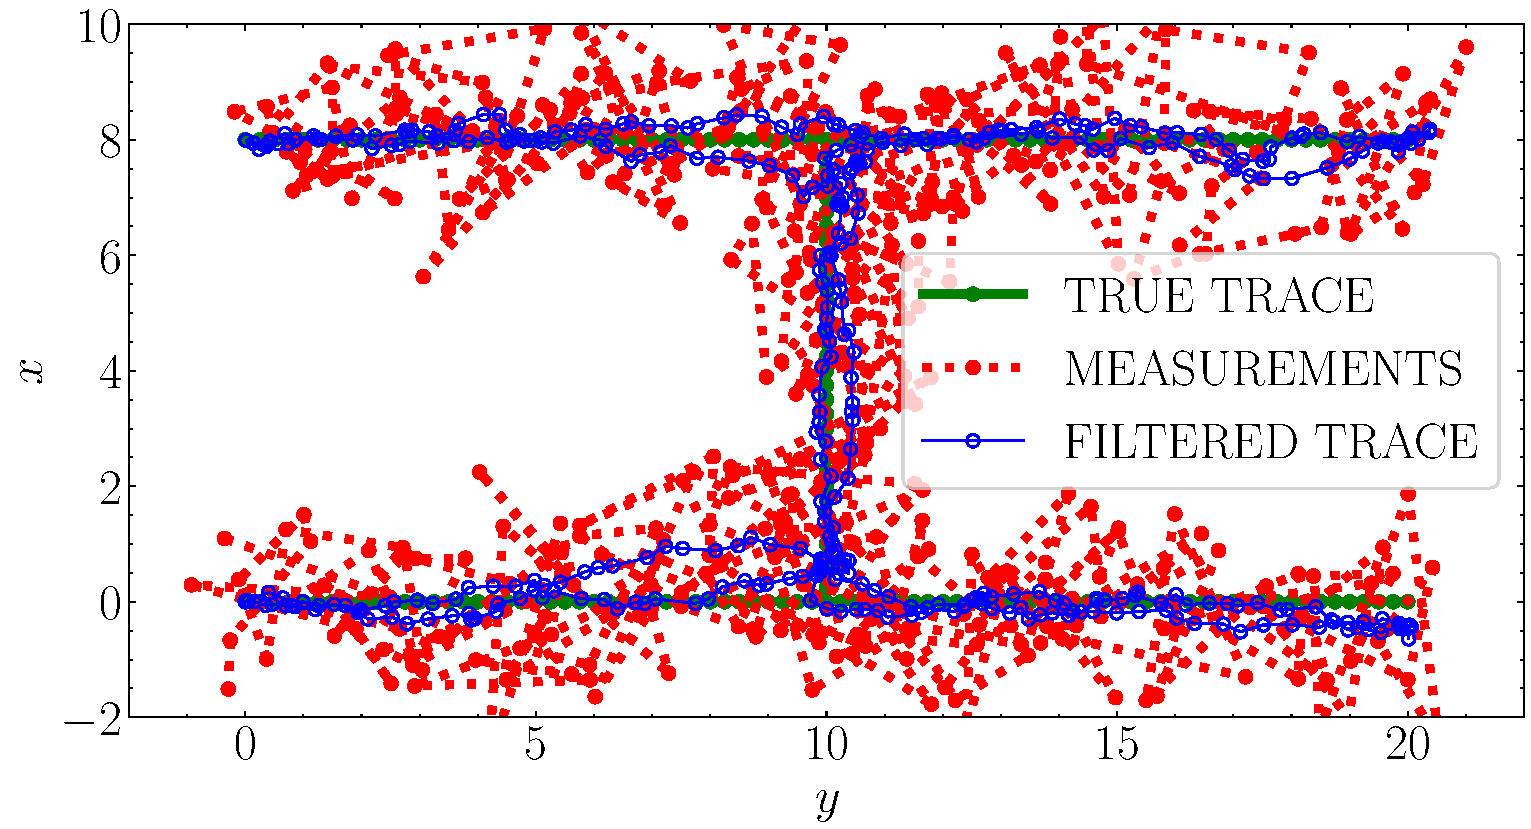
\includegraphics[width=3in]{../results/KF/ex3/KF_Pos_Trace_Data_high_noise_0.01}}
\subfigure[Error, $\bQ_{w}=0.01\bI$]{\label{fig:a}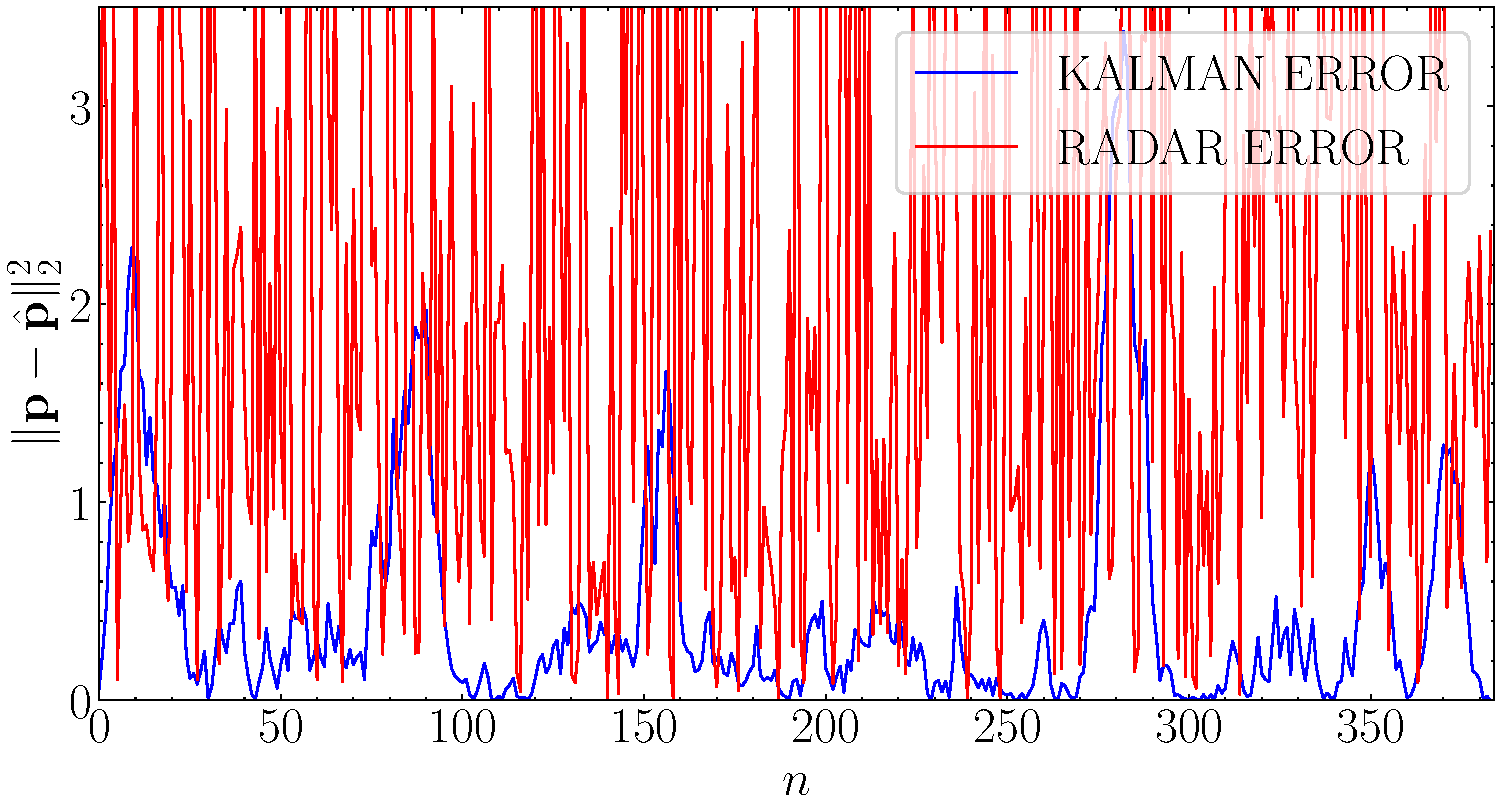
\includegraphics[width=3in]{../results/KF/ex3/KF_Pos_Errors_Data_high_noise_0.01}}

\subfigure[Trace $\bQ_{w}=0.1\bI$]{\label{fig:a}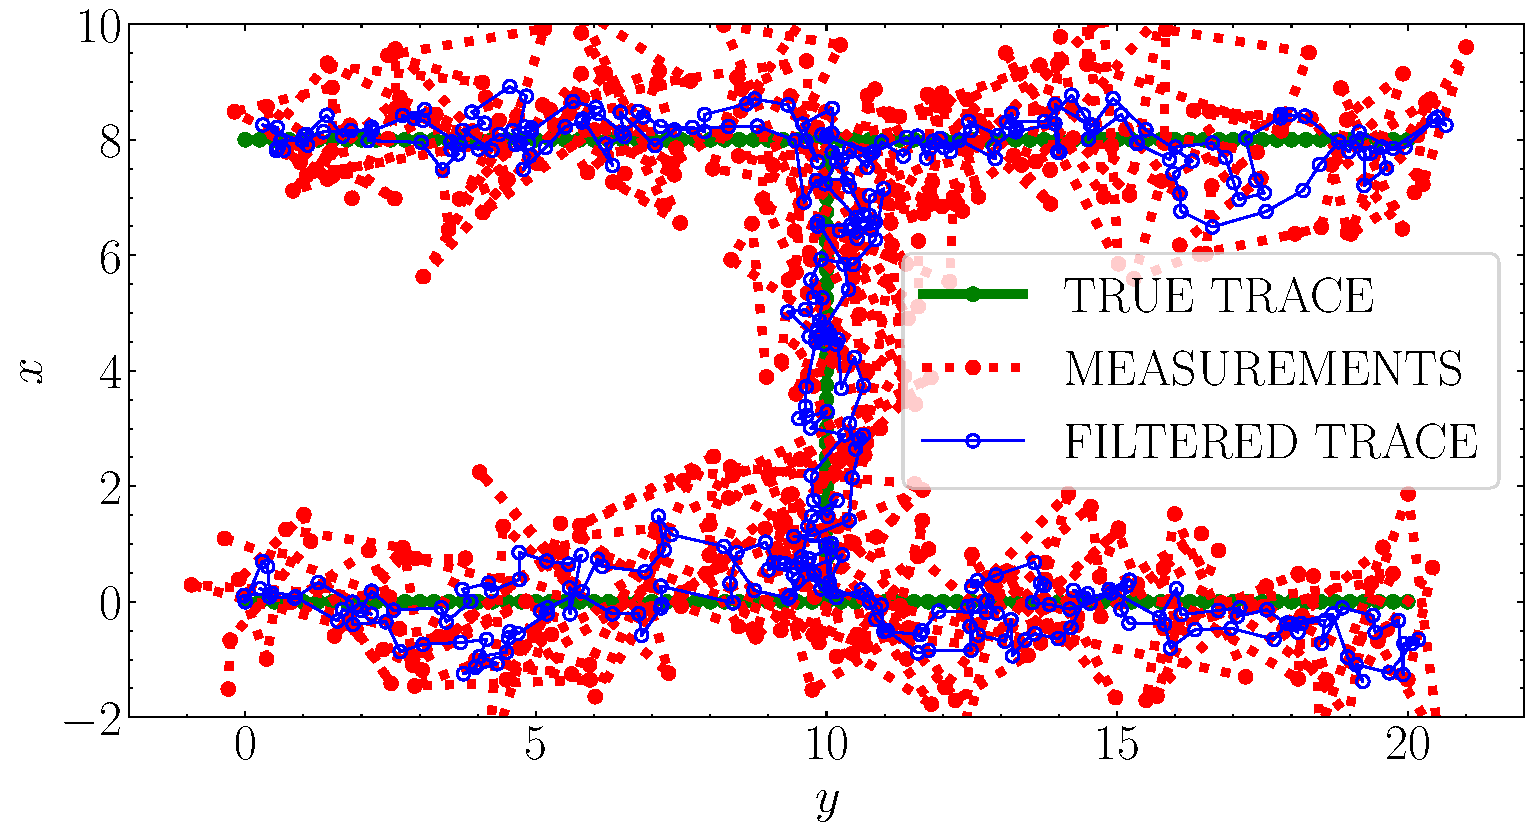
\includegraphics[width=3in]{../results/KF/ex3/KF_Pos_Trace_Data_high_noise_0.1}}
\subfigure[Error, $\bQ_{w}=0.1\bI$]{\label{fig:a}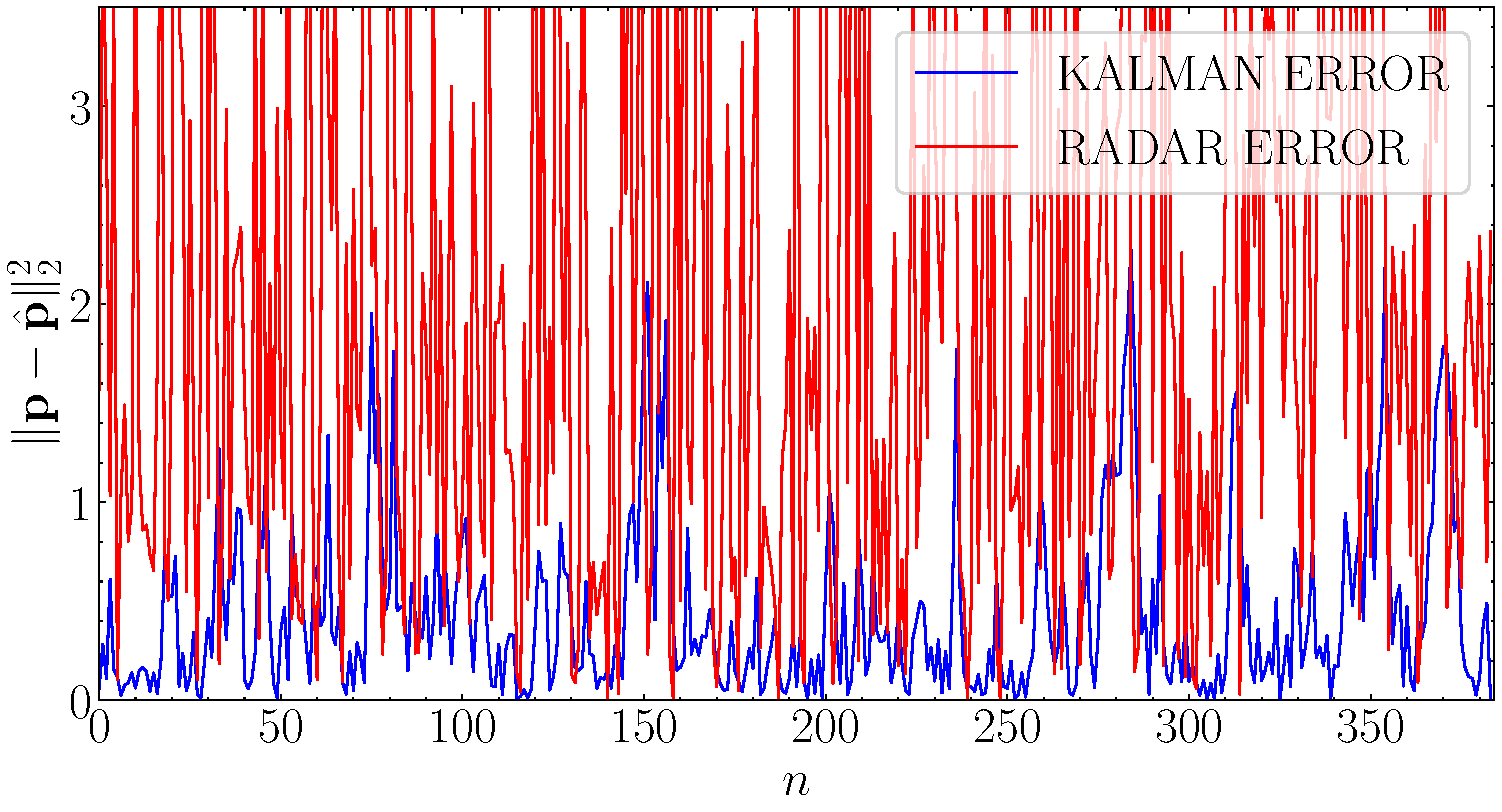
\includegraphics[width=3in]{../results/KF/ex3/KF_Pos_Errors_Data_high_noise_0.1}}

\subfigure[Trace $\bQ_{w}=\bI$]{\label{fig:a}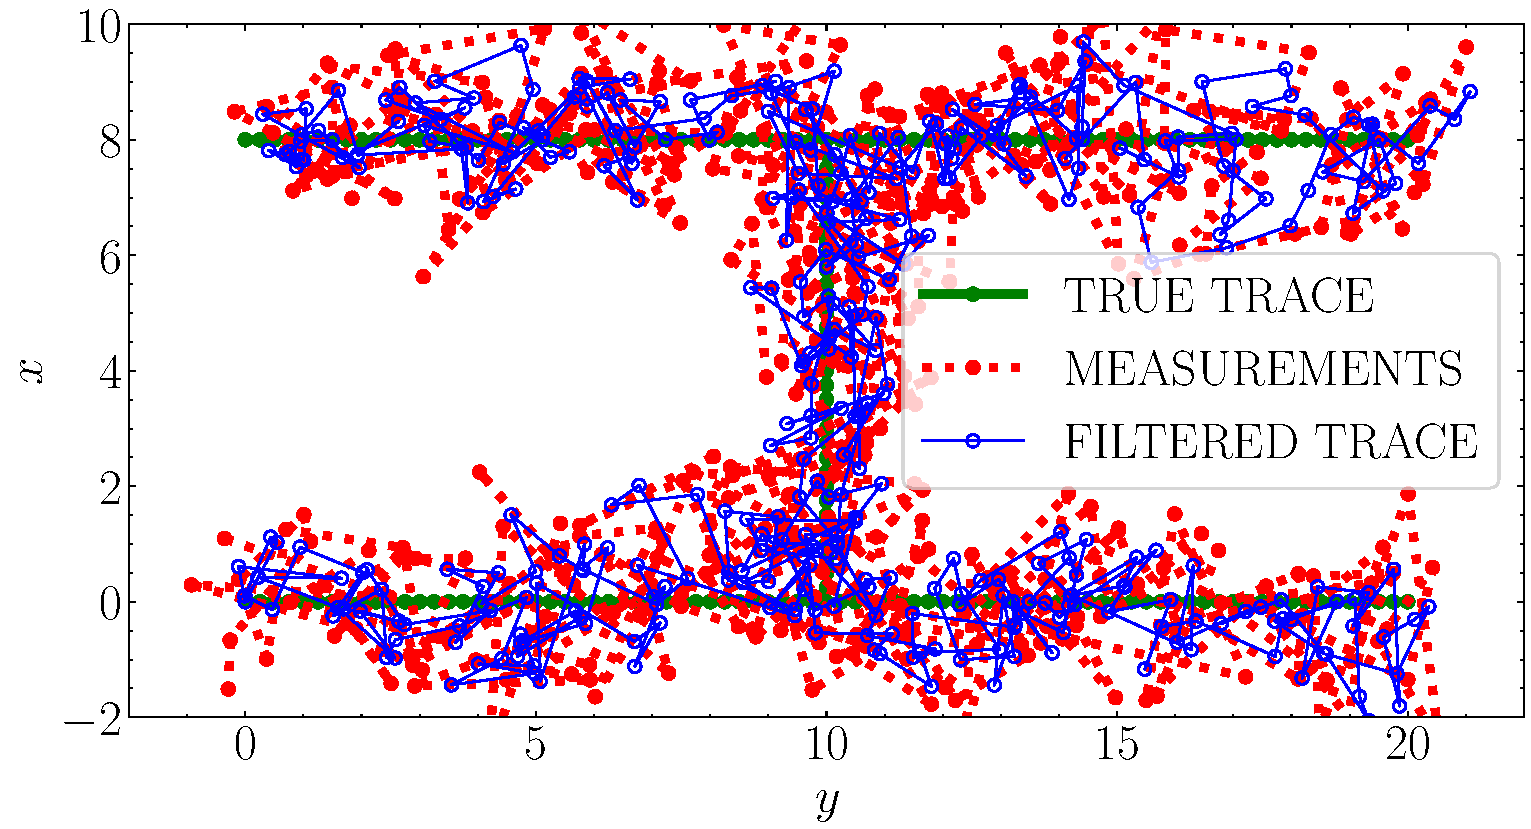
\includegraphics[width=3in]{../results/KF/ex3/KF_Pos_Trace_Data_high_noise_1.0}}
\subfigure[Error, $\bQ_{w}=\bI$]{\label{fig:a}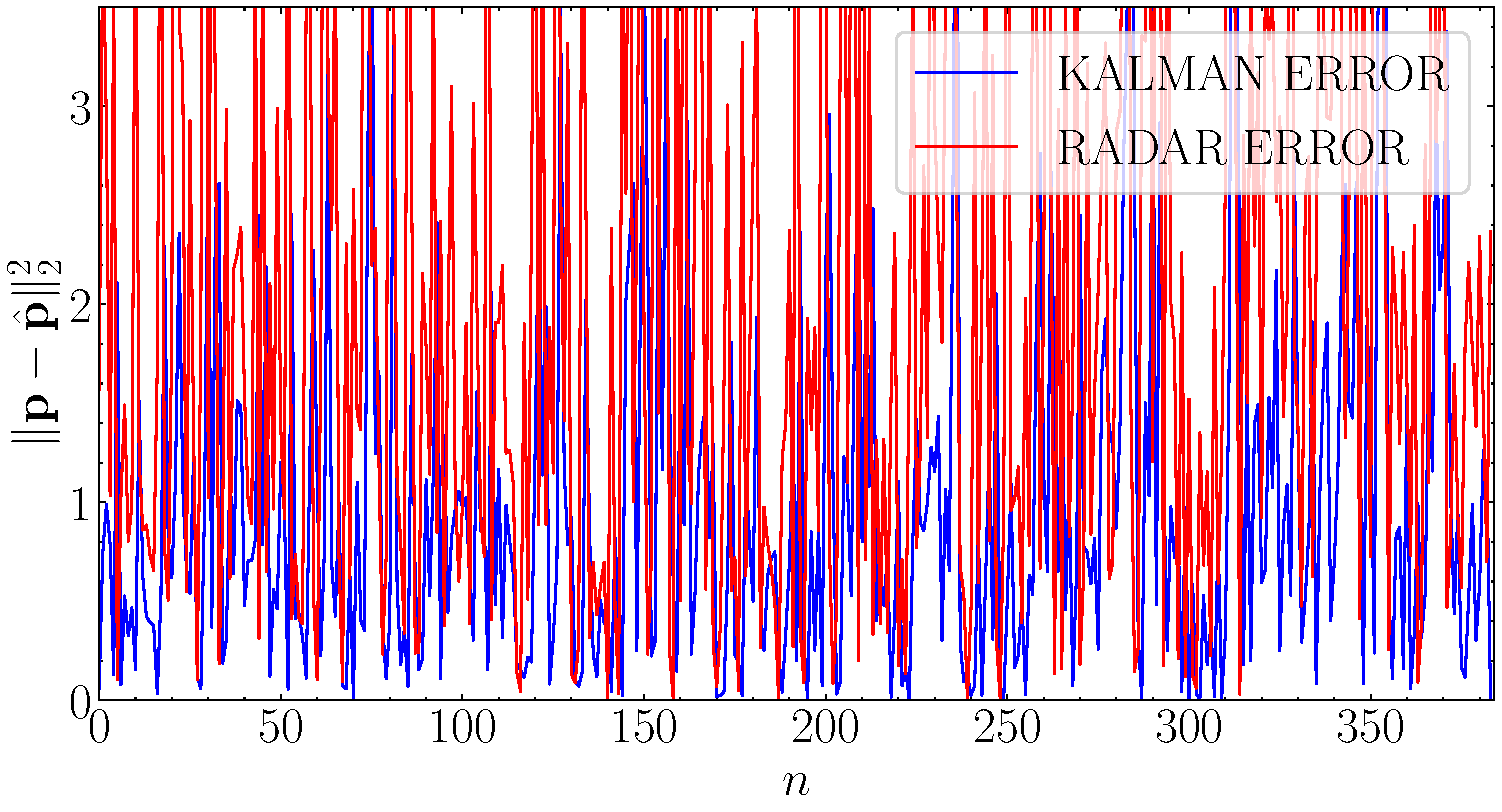
\includegraphics[width=3in]{../results/KF/ex3/KF_Pos_Errors_Data_high_noise_1.0}}
\caption{[Colour online] Figures show the Kalman filter prediction and RADAR measurements compared to the true trace. The first column shows the traces and the second column shows the errors, for different model noise, under measurements with $\bQ_{v}=\bI$.}
\label{fig:TraceVelPosHigh}
\end{figure}

Figure \ref{fig:TraceVelPosHigh} shows the trace and errors for the three cases of model noise. We observe the effect of model noise is stronger when the measurement noise is large. In the case where $\bQ_{v}=0.0001\bI$, the Kalman filter attempts to predict paths that are parallel to the axes, as not much model mismatch is allowed. Hence, due to the high measurement noise, the tracking is poor. This is clear with the Kalman filter error being much higher than the RADAR error. With $\bQ_{v}=0.01\bI, 0.1\bI$, the tracking improves as some model mismatch is allowed. The errors in the Kalman filter predictions are reasonable compared to the error in the RADAR measurements. Large errors are seen at time instants where the vehicle takes a turn as smooth turns are not accounted in the model. With $\bQ_{v} = \bI$, the model error is large and accommodates measurements including the noise in the measurements. The trace follows the measurements and captures the noise in the measurements. The errors in the Kalman filter predictions compare similar to the errors in the RADAR measurements. This is complete opposite to the case where $\bQ_{v}=0.0001\bI$. The model noise trades between fitting the measurements and obeying the model. The choice $\bQ_{v}=0.01\bI$ is a good choice for model noise as it trades well between obeying the model and denoising the measurements. This is clear by comparing the error in the Kalman filter predictions to the error in the RADAR measurements. In all cases, the error at time instants where the vehicle turns is large, as the model does not account for such motions. The choice $\bQ_{v}=0.01\bI$ gives the least error amongst these choices, for all other time instants.

% -----------------------------------------------------------------------------------------------------------------------

\subsubsection{Kalman filter with parameter mismatch}
\label{subsubsec:kalmanMismatch}

We implement the Kalman filter using both position and velocity measurements using the state model in (\ref{eq:kinematicsGeneral}) and measurement model as in (\ref{eq:stateMeasurements}). We consider RADAR measurements of both position and velocity with measurement noise $\bQ_{v}=\bI$. We fix the model noise with $\bQ_{w}=0.1\bI$ and consider Kalman filter predictions with model mismatch, taking $\bQ_{v} \in \{0.01\bI, 0.1\bI\}$. We initialise the Kalman filter with $\hat{x}[0|0] = \zerovec$, and determine the tracking performance using the squared-error between the Kalman filter predictions of position ($\hat{\mathbf{p}}[n]$) and the true trace ($\mathbf{p}[n]$), and compare it to the squared error between the RADAR measurements and the true trace.
\begin{figure}[h]
\centering
\subfigure[Trace $\bQ_{v}=0.01\bI$]{\label{fig:a}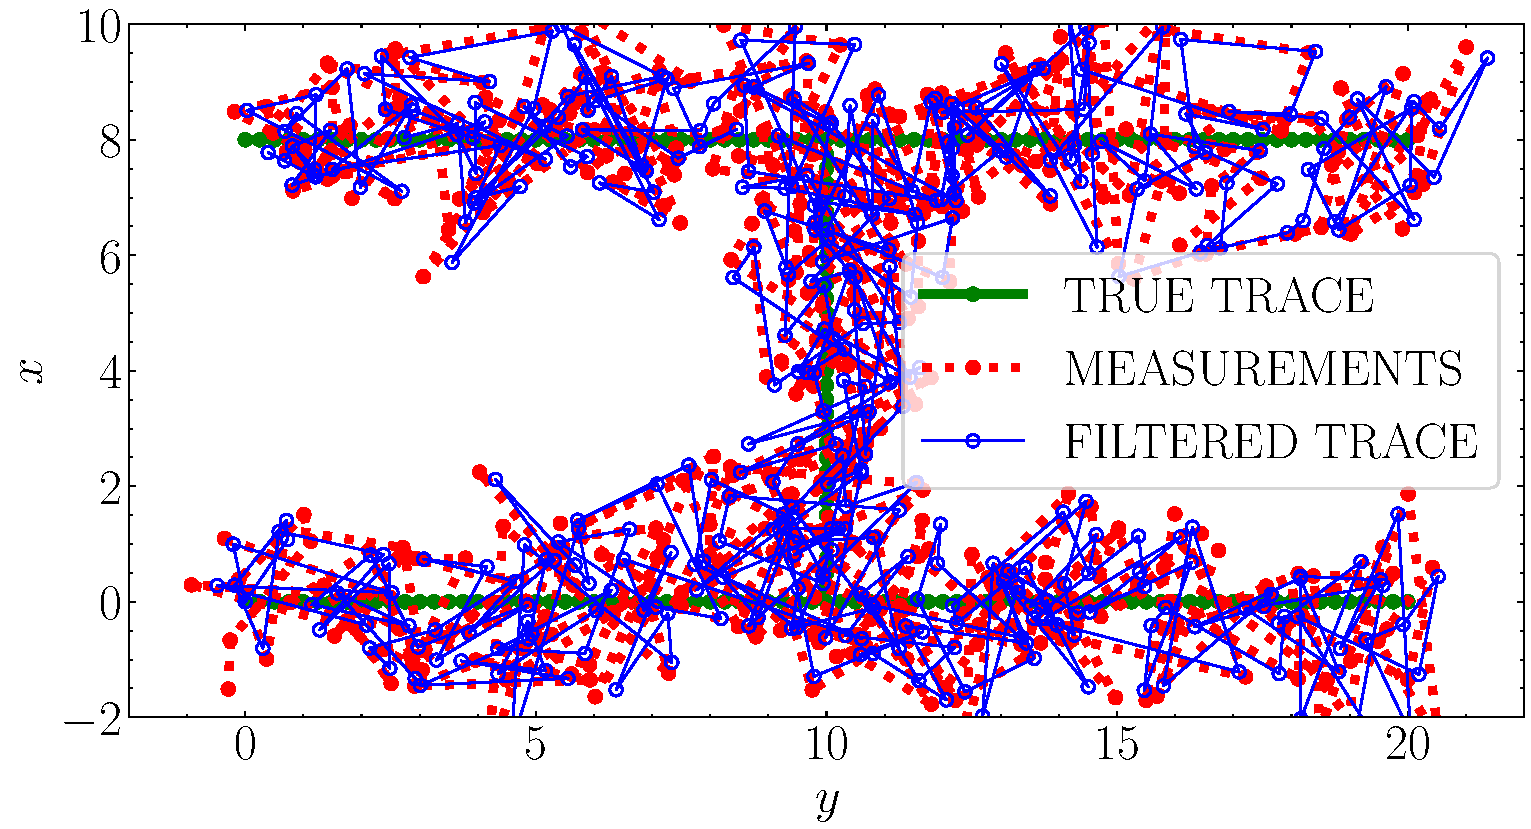
\includegraphics[width=3in]{../results/KF/ex4/KF_Pos_Trace_noise_0.01}}
\subfigure[Error, $\bQ_{v}=0.01\bI$]{\label{fig:a}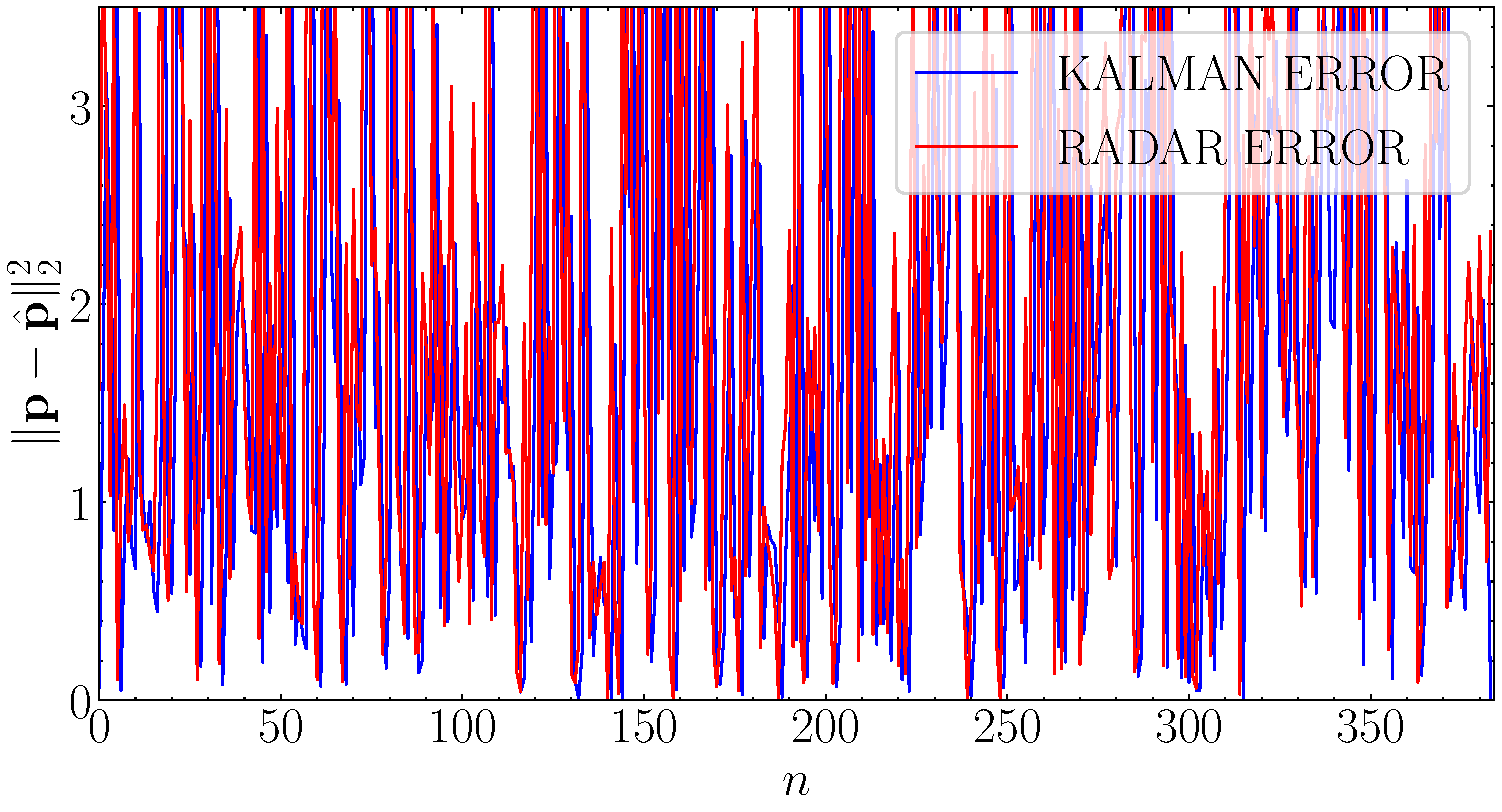
\includegraphics[width=3in]{../results/KF/ex4/KF_Pos_Errors_noise_0.01}}

\subfigure[Trace $\bQ_{v}=0.1\bI$]{\label{fig:a}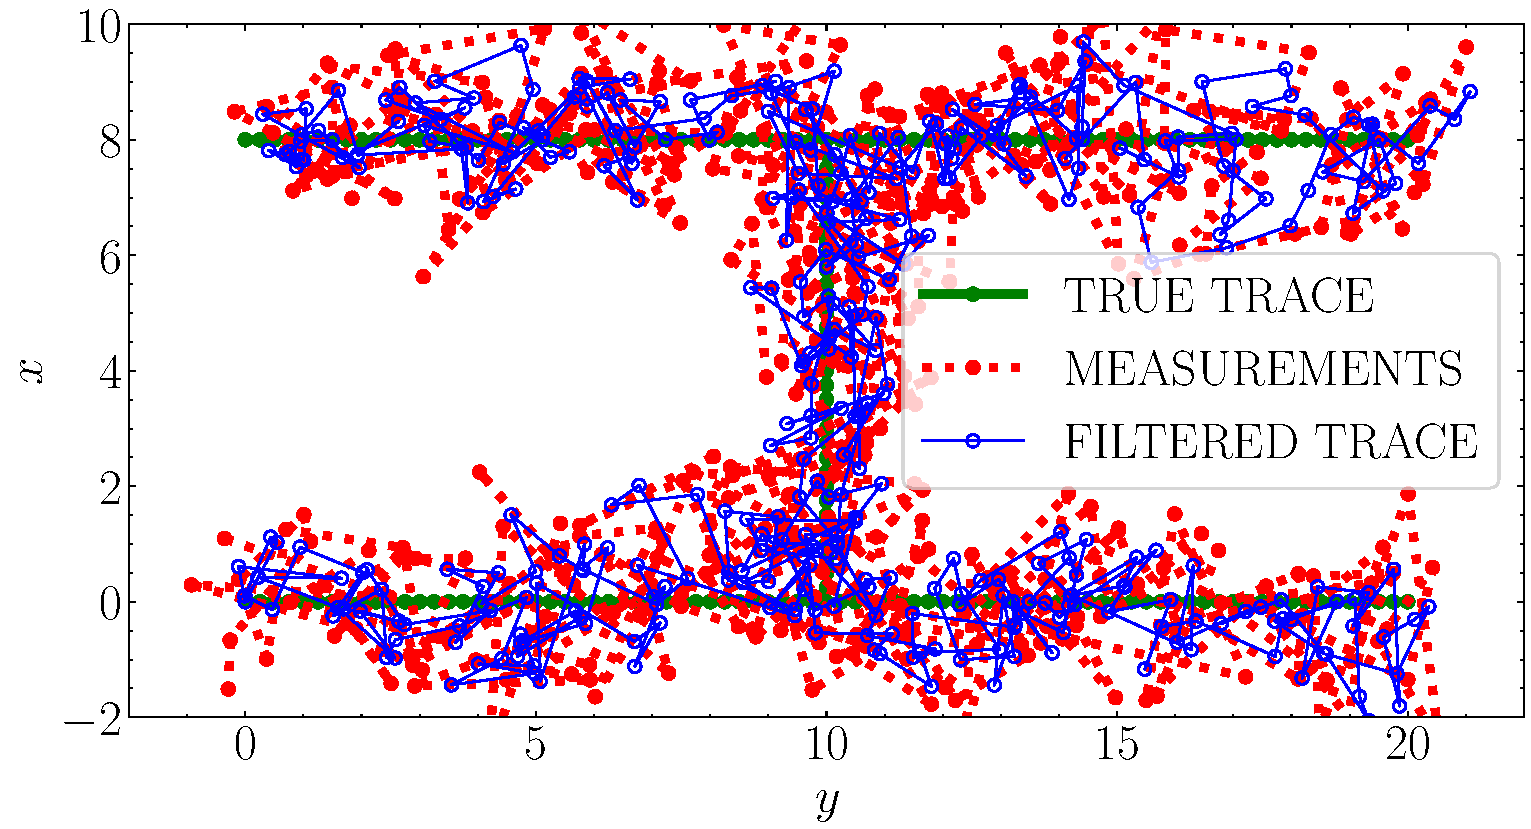
\includegraphics[width=3in]{../results/KF/ex4/KF_Pos_Trace_noise_0.1}}
\subfigure[Error, $\bQ_{v}=0.1\bI$]{\label{fig:a}\includegraphics[width=3in]{../results/KF/ex4/KF_Pos_Errors_noise_0.1}}

\caption{[Colour online] Figures show the Kalman filter prediction and RADAR measurements compared to the true trace. The first column shows the traces and the second column shows the errors, for different measurement noise (mismatched with the true parameter), under model with $\bQ_{w}=0.1\bI$.}
\label{fig:TraceVelPosHighMis}
\end{figure}

Figure \ref{fig:TraceVelPosHighMis} shows the trace and errors for the two cases of measurement noise. We observe that the tracking is poor in both cases. The Kalman filter updates, in Kalman gain, depend on the measurement statistics. The case where $\bQ_{v}=0.1\bI$ has lower error in the Kalman filter predictions as the mismatch in the parameter is smaller than the case where $\bQ_{v}=0.01\bI$.

As seen in Section \ref{subsubsec:kalmanNoisy}, the Kalman filter gives reliable tracking performance in presence of high measurement noise, if the model parameters are tuned well and the measurement statistics are known. If the measurement statistics are not known well, as seen in Figure \ref{fig:TraceVelPosHighMis}, the tracking performance will not be reliable, even in the case where the right model noise parameter is chosen from the results in Section \ref{subsubsec:kalmanNoisy}.


% -----------------------------------------------------------------------------------------------------------------------

\subsubsection{Kalman filter for automated driving test}
\label{subsubsec:kalmanTest}

We consider automating driving test using a Kalman filter with state model in (\ref{eq:kinematicsGeneral}) and measurement model as in (\ref{eq:stateMeasurements}). We consider the test measurements and assume measurement noise $\bQ_{v}=0.1\bI$, and choose the Kalman filter model with $\bQ_{w}=0.1\bI$. We track the vehicle using the Kalman filter predictions and flag the vehicle to fail the test if the Kalman filter prediction has an error larger than some threshold.

We want the vehicle to keep within the width of the track, i.e., we want $|p_{x}[n] - \hat{p}_{x}[n]|<1.25$ and $|p_{y}[n] - \hat{p}_{y}[n]|<1.25, \; \forall n$. This gives, $\Vert \hat{\mathbf{p}}[n] - \mathbf{p}[n] \Vert_{2}^{2} \leq 3.125$. Therefore, the test flags ``FAIL'' if the Kalman filter prediction error is more than $\tau = 3.125$ at any time instant, otherwise the test says ``PASS''.
\begin{figure}[!h]
\centering
\subfigure[Trace, Data 1]{\label{fig:a}\includegraphics[width=3in]{../results/KF/ex5/KF_Pos_Trace_Data_1}}
\subfigure[Error, Data 1]{\label{fig:a}\includegraphics[width=3in]{../results/KF/ex5/KF_Pos_Errors_Data_1}}

\subfigure[Trace, Data 2]{\label{fig:a}\includegraphics[width=3in]{../results/KF/ex5/KF_Pos_Trace_Data_2}}
\subfigure[Error, Data 2]{\label{fig:a}\includegraphics[width=3in]{../results/KF/ex5/KF_Pos_Errors_Data_2}}

\subfigure[Trace, Data 3]{\label{fig:a}\includegraphics[width=3in]{../results/KF/ex5/KF_Pos_Trace_Data_3}}
\subfigure[Error, Data 3]{\label{fig:a}\includegraphics[width=3in]{../results/KF/ex5/KF_Pos_Errors_Data_3}}

\subfigure[Trace, Data 4]{\label{fig:a}\includegraphics[width=3in]{../results/KF/ex5/KF_Pos_Trace_Data_4}}
\subfigure[Error, Data 4]{\label{fig:a}\includegraphics[width=3in]{../results/KF/ex5/KF_Pos_Errors_Data_4}}
\caption{[Colour online] Figures show the Kalman filter prediction and RADAR measurements compared to the true trace. The first column shows the traces and the second column shows the errors, for different test cases. The green line in the error plots depicts the threshold on the error to flag the test. The titles of the plot gives the result.}
\label{fig:TraceVelPosTest}
\end{figure}

Figure \ref{fig:TraceVelPosTest} shows the trace and errors for the four test cases. We observe the first, third and fourth cases ``PASS'', but the second case ``FAILS''. The error in the ``PASS'' cases never exceeds the threshold at any time instant, but the error in the second case exceeds the threshold over some intervals. This is also seen in the trace where the vertical section of the path is wrongly driven while the other cases drive approximately well.

% -----------------------------------------------------------------------------------------------------------------------
% -----------------------------------------------------------------------------------------------------------------------

\clearpage
\appendix

\subsection*{Scripts}

The Python3 scripts to generate all figures can be downloaded from the GitHub repository \url{https://github.com/kamath-abhijith/Vehicle_Tracking}. Use \texttt{requirements.txt} to install all dependencies, and the bash scripts to run the Python3 codes. Also, see the following code snippets for reference.

\subsubsection*{Implementation of $D_{\text{entry}}$}

The following script generates Figure \ref{fig:MCdentry}, \ref{fig:ROCdentry}. The relevant functions are in \texttt{utils.py}.
\lstinputlisting[language=Python]{../src/detect_entry.py}

% -----------------------------------------------------------------------------------------------------------------------

\subsubsection*{Implementation of $D_{\text{exit}}$}

The following script generates Figure \ref{fig:MCdexit}, \ref{fig:ROCdexit}. The relevant functions are in \texttt{utils.py}.
\lstinputlisting[language=Python]{../src/detect_exit.py}

% -----------------------------------------------------------------------------------------------------------------------
% -----------------------------------------------------------------------------------------------------------------------

\subsubsection*{Implementation of Kalman filter with velocity-only measurements}

The following script generates Figure \ref{fig:TraceVel}. The relevant functions are in \texttt{utils.py}.
\lstinputlisting[language=Python]{../src/track_vel.py}

% -----------------------------------------------------------------------------------------------------------------------

\subsubsection*{Implementation of Kalman filter with position and velocity measurements}

The following script generates Figure \ref{fig:TraceVelPosMed}, \ref{fig:TraceVelPosHigh}. The relevant functions are in \texttt{utils.py}.
\lstinputlisting[language=Python]{../src/track_pos.py}

% -----------------------------------------------------------------------------------------------------------------------

\subsubsection*{Implementation of Kalman filter with mismatched parameters}

The following script generates Figure \ref{fig:TraceVelPosHighMis}. The relevant functions are in \texttt{utils.py}.
\lstinputlisting[language=Python]{../src/track_mis.py}

% -----------------------------------------------------------------------------------------------------------------------

\subsubsection*{Implementation of Kalman filter to automate driving tests}

The following script generates Figure \ref{fig:TraceVelPosTest}. The relevant functions are in \texttt{utils.py}.
\lstinputlisting[language=Python]{../src/track_test.py}

% -----------------------------------------------------------------------------------------------------------------------

\subsubsection*{\texttt{utils.py}}

Use the \texttt{make trace video} to generate the video as shown in the presentation.
\lstinputlisting[language=Python]{../src/utils.py}

% -----------------------------------------------------------------------------------------------------------------------
% -----------------------------------------------------------------------------------------------------------------------

\end{document}
